\documentclass[
version=last,
toc=bib,
toc=graduated,
toc=index,
toc=listof,
fontsize=9pt,
parskip=false,
openany]{scrbook}
%\pdfminorversion=4
\usepackage[utf8]{inputenc}
\usepackage[ngerman]{babel}
\usepackage{fontspec}
\usepackage[default]{sourcesanspro}
\setfontfamily\dejavuSansFont{DejaVu Sans Condensed}

\usepackage{ifmtarg}
\usepackage{ifthen}
\usepackage{etoolbox} % \ifstrempty

\usepackage{geometry}
\geometry{%a6paper
  paperwidth=125mm,
  paperheight=168mm,
  portrait,
  top=22mm,
  inner=22mm,
  outer=20mm,
  bottom=25mm,
  headsep=3mm,
  footskip=12mm
}

\usepackage{ragged2e} % nicer typesetting (hyphenation) for non raggedright and raggedleft
\usepackage{lscape}
\setlength{\parskip}{0pt}

\usepackage{relsize}

\clubpenalty=10000 %keine Schusterjungen
\widowpenalty=10000 
\displaywidowpenalty=10000 % keine Hurenkinder

\usepackage[]{microtype}

\usepackage{graphicx} % graphics

% search path for images
\graphicspath{{images-print/}{icons/}}
\usepackage{wrapfig}  % sponsor logos wrapped with text

\usepackage{tabu}
\usepackage{tabularx}
\usepackage{longtable}
\usepackage[table,cmyk]{xcolor}
\usepackage{colortbl}

% embed PDF pages
% pdfpages must not be loaded before colortbl!
\usepackage{pdfpages}
% TikZ must not be loaded before colortbl
\usepackage{tikz}
\usetikzlibrary{calc}

% PDFs als Hintergrundbilder
\usepackage{multirow}
\usepackage{booktabs}
\usepackage{array}
\usepackage{varwidth}

\usepackage{refcount} % calculation of the page where the map is located
\usepackage{svg}



%\DeclareUnicodeCharacter{2032}{minutenstrich}

% page background
\usepackage[manualmark]{scrlayer-scrpage}
\pagestyle{scrplain}

\newcommand{\acro}[1]{{\textsmaller[0.5]{#1}}} % macro for abbreviations with more than one capitalised letter
\newcommand{\keeptabcolsep}{%
  \edef\restoretabcolsep{%
    \tabcolsep=\the\tabcolsep
  }%
}
\newcommand{\demotabcolsep}{%
  \setlength{\tabcolsep}{0.1em}
}%
% title/metadata
%\title{FOSSGIS-Konferenz 2023}
%\subtitle{Programm}
%\author{FOSSGIS e.V.}
%\date{\today}

\clearscrheadings

% page numbers
\cfoot[\begin{small}\pagemark\end{small}]{\begin{small}\pagemark\end{small}}
\ofoot[]{}
\ifoot[]{}
\pagestyle{scrplain}

% Durchschuss erhöhen
\linespread{1.15}

\begin{document}

% include our custom macros
% command for a new time slot
\newcommand{\talkTime}{9:99}
\newcommand{\newTimeslot}[1]{\newpage\renewcommand{\talkTime}{#1}}

% new time slot but without a pagebreak
\newcommand{\newSmallTimeslot}[1]{\renewcommand{\talkTime}{#1}}

% new time slot for Lightning Talk
\newcommand{\newLightningTimeslot}[1]{\renewcommand{\talkTime}{#1 (LT)}}

% initialise \conferenceDay 
\newcommand{\conferenceDay}{Noday}


\input{wallpaper/day-layers.tex}

% define page style for cutting marks without anything else
\DeclareNewLayer[background, oddorevenpage, width=125mm,%
height=169mm, contents={%
  \begin{tikzpicture}[x=1mm, y=1mm]
    \drawCropMarks
  \end{tikzpicture}
}]{cropmarksplain}

% define default page style (cutting marks with page number)
\DeclareNewLayer[background, oddorevenpage, width=125mm,%
height=169mm, contents={%
  \begin{tikzpicture}[x=1mm, y=1mm]
    \drawCropMarks
  \end{tikzpicture}
}]{cropmarksevery}
\newpairofpagestyles[scrheadings]{cropmarksstyle}{}
\AddLayersAtBeginOfPageStyle{cropmarksstyle}{cropmarksevery}

% page style for title pages
\DeclareNewLayer[background, oddorevenpage, width=125mm,%
height=169mm, contents={%
  \includegraphics{wallpaper/front-cover-with-crop-marks.pdf}%
}]{titlelayer}
\newpairofpagestyles[]{titlestyle}{}
\AddLayersAtBeginOfPageStyle{titlestyle}{titlelayer}

% define alias commands for all three days
\def\mittwoch{Mittwoch}
\def\donnerstag{Donnerstag}
\def\freitag{Freitag}
\def\samstag{Samstag}

% define Mittwoch page style
\newpairofpagestyles[scrheadings]{mittwoch-table}{}
\AddLayersAtBeginOfPageStyle{mittwoch-table}{mittwocheven}
\AddLayersAtBeginOfPageStyle{mittwoch-table}{mittwochoddrotated}
\newpairofpagestyles[scrheadings]{mittwoch}{}
\AddLayersAtBeginOfPageStyle{mittwoch}{mittwocheven}
\AddLayersAtBeginOfPageStyle{mittwoch}{mittwochodd}

% define Donnerstag page style
\newpairofpagestyles[scrheadings]{donnerstag-table}{}
\AddLayersAtBeginOfPageStyle{donnerstag-table}{donnerstageven}
\AddLayersAtBeginOfPageStyle{donnerstag-table}{donnerstagoddrotated}
\newpairofpagestyles[scrheadings]{donnerstag}{}
\AddLayersAtBeginOfPageStyle{donnerstag}{donnerstageven}
\AddLayersAtBeginOfPageStyle{donnerstag}{donnerstagodd}

% define Freitag page style
\newpairofpagestyles[scrheadings]{freitag-table}{}
\AddLayersAtBeginOfPageStyle{freitag-table}{freitageven}
\AddLayersAtBeginOfPageStyle{freitag-table}{freitagoddrotated}
\newpairofpagestyles[scrheadings]{freitag}{}
\AddLayersAtBeginOfPageStyle{freitag}{freitageven}
\AddLayersAtBeginOfPageStyle{freitag}{freitagodd}

% define Samstag page style
\newpairofpagestyles[scrheadings]{samstag-table}{}
\AddLayersAtBeginOfPageStyle{samstag-table}{samstageven}
\AddLayersAtBeginOfPageStyle{samstag-table}{samstagoddrotated}
\newpairofpagestyles[scrheadings]{samstag}{}
\AddLayersAtBeginOfPageStyle{samstag}{samstageven}
\AddLayersAtBeginOfPageStyle{samstag}{samstagodd}

% \setpagebackground selects the page style to be used depending on the current day. Each day has
% its own page style.
\newcommand{\setPageBackground}{%
  \ifthenelse{\equal{\conferenceDay}{\mittwoch}}{%
    \pagestyle{mittwoch}%
  }{}%
  \ifthenelse{\equal{\conferenceDay}{\donnerstag}}{%
    \pagestyle{donnerstag}%
  }{}%
  \ifthenelse{\equal{\conferenceDay}{\freitag}}{%
    \pagestyle{freitag}%
  }{}%
  \ifthenelse{\equal{\conferenceDay}{\samstag}}{%
    \pagestyle{samstag}%
  }{}%
}


% additional column type for tables
\newcolumntype{Y}[1]{>{\RaggedRight\arraybackslash}p{#1}}

%% length of the title boxes
\newlength{\titleboxwidth}
\setlength{\titleboxwidth}{\textwidth}
\advance\titleboxwidth by -6pt

\newlength{\roomWidth}
\newlength{\timeWidth}
\newlength{\roomTimeWidth}
\newlength{\titleWidth}
\newcommand{\tmpRoomTimeWidth}{}
\newcommand{\tmpTitleWidth}{}

\DeclareRobustCommand*{\setAbstract}[6]{%
  % 1. speaker
  % 2. title
  % 3. subtitle
  % 4. abstract (Text)
  % 5. colour
  % 6. room
  \setPageBackground%
  \calculateRoomTimeAndTitleWidth{#1}{#6}%
  \noindent\fcolorbox{white}{#5}{%
    \noindent\parbox{\titleboxwidth}{%
      \isSpeakerEmpty{#1}{#2}{#6}%
      \isSubtitleEmpty{#3}%
    }%
  }%
  %
  \justifying
  \isAbstractEmpty{#4}%
  \vspace{0.5em}% space to the next talk even if there is no abstract
}

% Calculate width of title and room/time field
% Arguments: speaker, room
\makeatletter
  \newcommand{\calculateRoomTimeAndTitleWidth}[2]{%
    \@ifmtarg{#1}{% speaker is empty
      \settowidth{\roomWidth}{#2, \talkTime}%
    }{% speaker is not empty
      \settowidth{\roomWidth}{#2}%
    }%
    \settowidth{\timeWidth}{\talkTime}%
    \directlua{require("lua/titleWidth")}%
    \setlength{\titleboxwidth}{\directlua{getTitleBoxWidth()}}%
    \renewcommand{\tmpRoomTimeWidth}{\directlua{getTimeRoomWidth()}}%
    \setlength{\roomTimeWidth}{\tmpRoomTimeWidth}%
    \renewcommand{\tmpTitleWidth}{\directlua{getTitleWidth()}}%
    \setlength{\titleWidth}{\tmpTitleWidth}%
  }%
\makeatother

% Lay out the subtitle
% has to be a separate function and has to be surrounded by \makeatletter for technical reasons
\makeatletter
  \newcommand{\isSubtitleEmpty}[1]{%
    \@ifnotmtarg{#1}{%
      \par
      \RaggedRight
      \vspace{0.3\baselineskip}
      \noindent%
      \bfseries%
      #1%
    }
  }
\makeatother

% lay out the speaker if there is any
% We assume that there is only a subtitle if the talk has a speaker.
\makeatletter
  \newcommand{\isSpeakerEmpty}[3]{%
    % Arguments:
    % 1. speaker
    % 2. title
    % 3. room
    \@ifmtarg{#1}{%
      \begin{minipage}[t][][t]{\titleWidth}
        \RaggedRight
        \noindent%
        {\large \sectfont #2}%
      \end{minipage}%
      \hfill
      \begin{minipage}[t][][t]{\roomTimeWidth}
        \RaggedLeft%
        \noindent #3, \talkTime%
      \end{minipage}%
    }%
    {%
      \begin{minipage}[t][][t]{\titleWidth}
        \RaggedRight
        \noindent
        \emph{#1} % speaker
        \par%
        \noindent%
        {\large \sectfont #2}%
      \end{minipage}%
      \hfill
      \begin{minipage}[t][][t]{\roomTimeWidth}
        \RaggedLeft
        \noindent
        \talkTime%
        \par%
        \noindent #3% room
      \end{minipage}%
    }%
  }
\makeatother

% Lay out the abstract if there is any
% has to be a separate function and has to be surrounded by \makeatletter for technical reasons
\makeatletter
\newcommand{\isAbstractEmpty}[1]{%
  \ifstrempty{#1}{%
    \vspace{1.5em}%
  }{%
    \vspace{0.5em}\newline%
    #1 \par% % abstract
    \vspace{1.5em}% space to the next talk even if there is an abstract
  }%
}
\makeatother

% define colours
%\definecolor{eins}{cmyk}{0 .18 .06 .10}
\definecolor{eins}{cmyk}{0 .13 .04 .08}
\definecolor{zwei}{cmyk}{.1 0 .17 .05}
\definecolor{hellorange}{cmyk}{0 0.18 0.40 0.03}
\definecolor{audimax}{cmyk}{0.13 0 0.04 0.11}
\definecolor{geoblau}{cmyk}{0.24 .02 0 .01}
\definecolor{dezentrot}{cmyk}{0 .24 0.29 .04}
\definecolor{hellgelb}{cmyk}{0 .02 0.36 0}
\definecolor{hellgruen}{cmyk}{0.10 .0 0.22 0.05}

% abstract at HS 1
\DeclareRobustCommand*{\abstractHSeins}[4]%
{%
  \setAbstract{#1}{#2}{#3}{#4}{geoblau}{HS~1 (Aula)}
}
% table heading for HS 1
\newcommand{\HSeins}{\cellcolor{geoblau} HS~1 (Aula)}

% abstract at HS 2
\DeclareRobustCommand*{\abstractHSzwei}[4]%
{%
  \setAbstract{#1}{#2}{#3}{#4}{hellgelb}{HS~2 (S10)}
}
% table heading for HS 2
\newcommand{\HSzwei}{\cellcolor{hellgelb} HS~2 (S10)}

% abstract at HS 3
\DeclareRobustCommand*{\abstractHSdrei}[4]%
{%
  \setAbstract{#1}{#2}{#3}{#4}{hellgruen}{HS~3 (S1)}
}
% table heading for HS 3
\newcommand{\HSdrei}{\cellcolor{hellgruen} HS~3 (S1)}

% abstract at HS 4
\DeclareRobustCommand*{\abstractHSvier}[4]%
{%
  \setAbstract{#1}{#2}{#3}{#4}{dezentrot}{HS~4 (S2)}
}
% table heading for HS 4
\newcommand{\HSvier}{\cellcolor{dezentrot} HS~4 (S2)}

% abstract at Anwendertreffen | BoF1 (S~8)
\DeclareRobustCommand*{\abstractAnwBoFeins}[4]%
{%
  \setAbstract{#1}{#2}{#3}{#4}{eins}{Anw./BoF1 (S8)}
}
% table heading for BoF1 
\newcommand{\BoFeins}{\cellcolor{eins}\small Anw.\,/\,BoF\,1\,(S8)}

% abstract at Anwendertreffen | BoF2 (S~9)
\DeclareRobustCommand*{\abstractAnwBoFzwei}[4]%
{%
  \setAbstract{#1}{#2}{#3}{#4}{zwei}{Anw./BoF2 (S9)}
}
% table heading for BoF2 
\newcommand{\BoFzwei}{\cellcolor{zwei}\small Anw.\,/\,BoF\,2\,(S9)}

% abstract at Anwendertreffen | BoF3/Exp (Sen.)
\DeclareRobustCommand*{\abstractAnwBoFdrei}[4]%
{%
  \setAbstract{#1}{#2}{#3}{#4}{audimax}{BoF3/Exp. (Senatssaal)}
}
% table heading for BoF3/Exp
\newcommand{\BoFdrei}{\cellcolor{audimax}\small Exp.\,/\,BoF\.3\,(Senatss.)}

% abstract at a different location
\newcommand{\abstractOther}[5]%
{%
  \setAbstract{#1}{#2}{#3}{#4}{hellorange}{#5}
}

% infobox for workshops (they don't have an abstract in the booklet)
\newcommand{\workshopbox}[3]{%
  % 1. titel
  % 2. speaker
  % 3. Room
  \setlength\tabcolsep{2pt}%
  \noindent\fcolorbox{white}{dezentrot}{%
    \parbox{\titleboxwidth}{%
      \noindent%
      \begin{tabu}{X[5L]r}
        \emph{#2} % Sprecher
        &
        \talkTime
        \tabularnewline
        {\noindent\large \bfseries #1}% % title
        &
        #3
        \tabularnewline
      \end{tabu}
    }
  }
  \setlength\tabcolsep{6pt} % set column padding back to default
}

% too long
\newcommand{\tooLong}{Dieser Text ist viel zu lang. Dieser Text ist viel zu lang. Dieser Text ist viel zu lang. Dieser Text ist viel zu lang. Dieser Text ist viel zu lang. Dieser Text ist viel zu lang. Dieser Text ist viel zu lang. Dieser Text ist viel zu lang. Dieser Text ist viel zu lang. Dieser Text ist viel zu lang. Dieser Text ist viel zu lang. Dieser Text ist viel zu lang. Dieser Text ist viel zu lang. Dieser Text ist viel zu lang. }

\newlength{\fboxwidth}

\def\workshopsSection{workshopsSection}
\def\abstractsSection{abstractsSection}

% boxes for text-only advertisement texts by our sponsors
\newcommand{\sponsorBox}[4]{%
  \setlength{\fboxwidth}{\textwidth}
  \advance\fboxwidth by -7.0pt
  \abstractSponsorbox{#1}{#2}{#3}{#4}{\workshopsSection}%
}

\newcommand{\sponsorBoxA}[4]{%
  \setlength{\fboxwidth}{\textwidth}%
  \advance\fboxwidth by -10.0pt%
  \abstractSponsorbox{#1}{#2}{#3}{#4}{\abstractsSection}%
}

\newcommand{\sponsorBoxLandscape}[4]{%
  \setlength{\fboxwidth}{\linewidth}
  \advance\fboxwidth by -10.0pt
  \abstractSponsorbox{#1}{#2}{#3}{#4}{\abstractsSection}%
}

%% store \parindent in separate variable because it is resetted to 0 in parboxes
\newlength{\saveparindent}
\setlength{\saveparindent}{\parindent}

%% box for advertisment by a sponsor
%% 1. logo (leave empty if none)
%% 2. width of the logo (leave empty if none
%% 3. number of required lines of the logo (due to usage of wrapfigure)
%% 4. text
%% 5. where we are in the booklet (\workshopsSection or \abstractsSection}
\makeatletter
  \newcommand{\abstractSponsorbox}[5]{%
    \setlength{\fboxsep}{4.5pt}%
    \noindent%
    \ifthenelse{\equal{#5}{\workshopsSection}}{%
      \hspace{2.65pt}%
    }{%
      \hspace{-1pt}%
    }%
    \fcolorbox{gray}{white}{%
      \parbox{\fboxwidth}{%
        \setlength{\parindent}{\saveparindent}%
        \@ifmtarg{#1}{}{%
          \begin{wrapfigure}[#3]{r}[0pt]{#2}%
            \centering\vspace{-1\baselineskip}%
            \includegraphics[width=#2]{#1}%
          \end{wrapfigure}%
        }%

        \noindent #4
      }%
    }%
    \setlength{\fboxsep}{3pt}%
  }%
  \setlength{\fboxsep}{3pt}%
\makeatother

% definition of column types for the schedule tables
\newcolumntype{Z}[1]{>{\RaggedRight\arraybackslash}p{#1}}%
\newcolumntype{C}[1]{>{\Centering\arraybackslash}p{#1}}%

% common implementation of typesetting of a session in the tables
\newcommand{\talkInternal}[2]{%
  \textbf{#1}
  \ifthenelse{\equal{#2}{}}{}{%
    \newline\emph{#2}%
  }
}

% common implementation of typesetting of a session in the tables -- singleline mode
\newcommand{\talkInternalSingleLine}[2]{%
  \textbf{#1}
  \hspace{0.5em}
  \ifthenelse{\equal{#2}{}}{}{%
    \emph{#2}%
  }
}

% macro to typeset a talk in the schedule tables spanning over more than one row:
% usage: \longTalk{rowcount}{title}{speaker}
\newcommand{\longTalk}[3]{%
  &
  \multirow{#1}{\linewidth}{%
    \parbox{\linewidth}{
      %HACK Inserting a \vspace here is a dirty hack but it works.
      \vspace{0.45\baselineskip}
      \talkInternal{#2}{#3}%
    }
  }%
}%

% macro to typeset a talk in the schedule tables:
% usage: \talk{title}{speaker}
\newcommand{\talk}[2]{%
  &
  \talkInternal{#1}{#2}%
}%

% macro to typeset a talk in the schedule tables, single line mode:
% usage: \talkSingleLine{title}{speaker}
\newcommand{\talkSingleLine}[2]{%
  &
  \talkInternalSingleLine{#1}{#2}%
}%


% macro to typeset a talk in the schedule tables spanning over more than one column:
% usage: \multiColTalk{columns}{columnSpecs}{title}{speaker}
\newcommand{\multiColTalk}[4]{%
  &
  \multicolumn{#1}{#2}{\talkInternal{#3}{#4}}%
}%

% set time in scheduel table
\newcommand{\tableRowFirstCell}[1]{%
  \cellcolor{table-header}
  \textcolor{black}{#1}%
}

% set time in scheduel table
\newcommand{\tableColHead}[1]{%
  \cellcolor{table-header}%
  \textcolor{black}{#1}%
}

\newcommand{\workshop}[3]%
{%
  \workshopbox{#1}{#2}{#3}%
}%

\newcommand{\otherevent}[1]%
{%
  & \textbf{#1}
}%

\newcommand{\audimaxEvent}[2]%
{%
  &
  \multicolumn{3}{c}{
    \textbf{#1} (Audimax) \par \emph{#2}
  }
}%

\newcommand{\coffeespace}{\vspace{0.4em}}
\newcommand{\workshopspace}{\vspace{0.5em}\\}

% define colors
\definecolor{commongray}{gray}{.9}
\definecolor{tableRuleGray}{gray}{.9}
\definecolor{textGray}{gray}{.45}

% macro for table rules
\newcommand{\programCRule}[1]{%
  \cline{#1}%
}
\newcommand{\programHRule}[1]{%
  \cline{2-#1}%
}

% macro for empty session slots
\newcommand{\bookableSpace}{
  & \emph{\textcolor{textGray}{Bookable Space}}%
}

% diamond symbol for shortened titles
\newcommand{\diamondSymbol}{%
  \textsuperscript{%
    \diamond%
  }%
}

% speaker affiliation
\newcommand{\speakerAffiliation}[1]{%
  (#1)%
}

% lightning talk (title and author)
\newcommand{\lightningTalk}[2]{%
  \item \emph{#2:} #1%
}

% macro for no-video icon
\newcommand{\noVideo}{%
  \raisebox{-0.2\height}{%
    \includegraphics[height=8pt]{novideo.pdf}%
  }%
}

% Titelseite
\DeclareNewLayer[background,%
%  width=115mm,%
 % height=158mm,%
% hoffset=5mm,%
% voffset=5mm,%
  width=115mm,%
  height=158mm,%
  hoffset=10mm,%
  voffset=10mm,%
  contents={%
   \begin{tikzpicture}[x=1mm, y=1mm]%
      % map image
      \draw (0,0) node [inner sep=0mm, anchor=south west] {%
        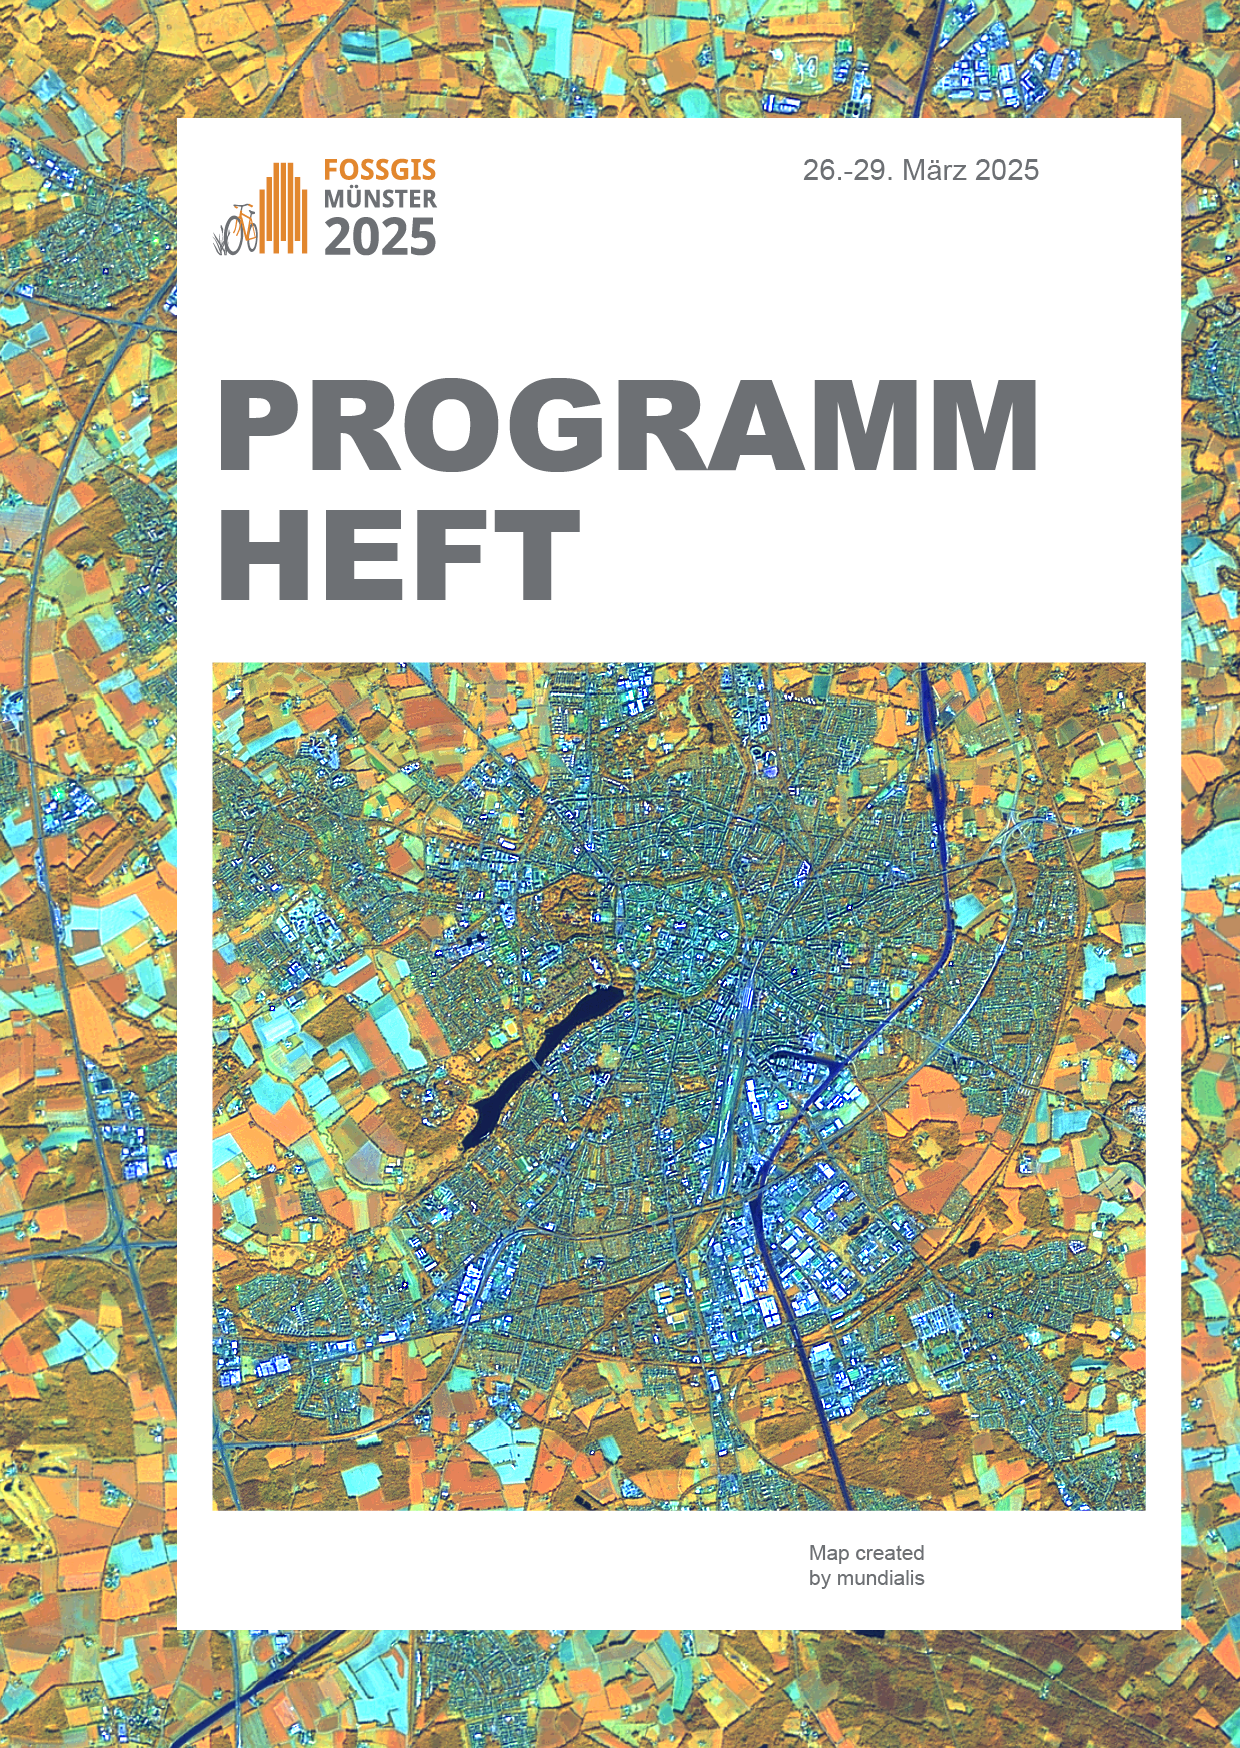
\includegraphics[height=148mm]{images-print/250217_fossgis25_programmheft_cover.png}%
      };%
      \end{tikzpicture}%
   }%
]{titelseite}
\newpairofpagestyles[]{page-title}{}
\AddLayersAtBeginOfPageStyle{page-title}{titelseite}
\AddLayersAtBeginOfPageStyle{page-title}{cropmarksplain}

% Übersicht alle Häuser 
\DeclareNewLayer[background,%
  width=115mm,%
  height=158mm,%
  hoffset=10mm,%
  voffset=10mm,%
  contents={%
    \begin{tikzpicture}[x=1mm, y=1mm]%
      % map image
      \draw (0,0) node [inner sep=0mm, anchor=south west] {%
        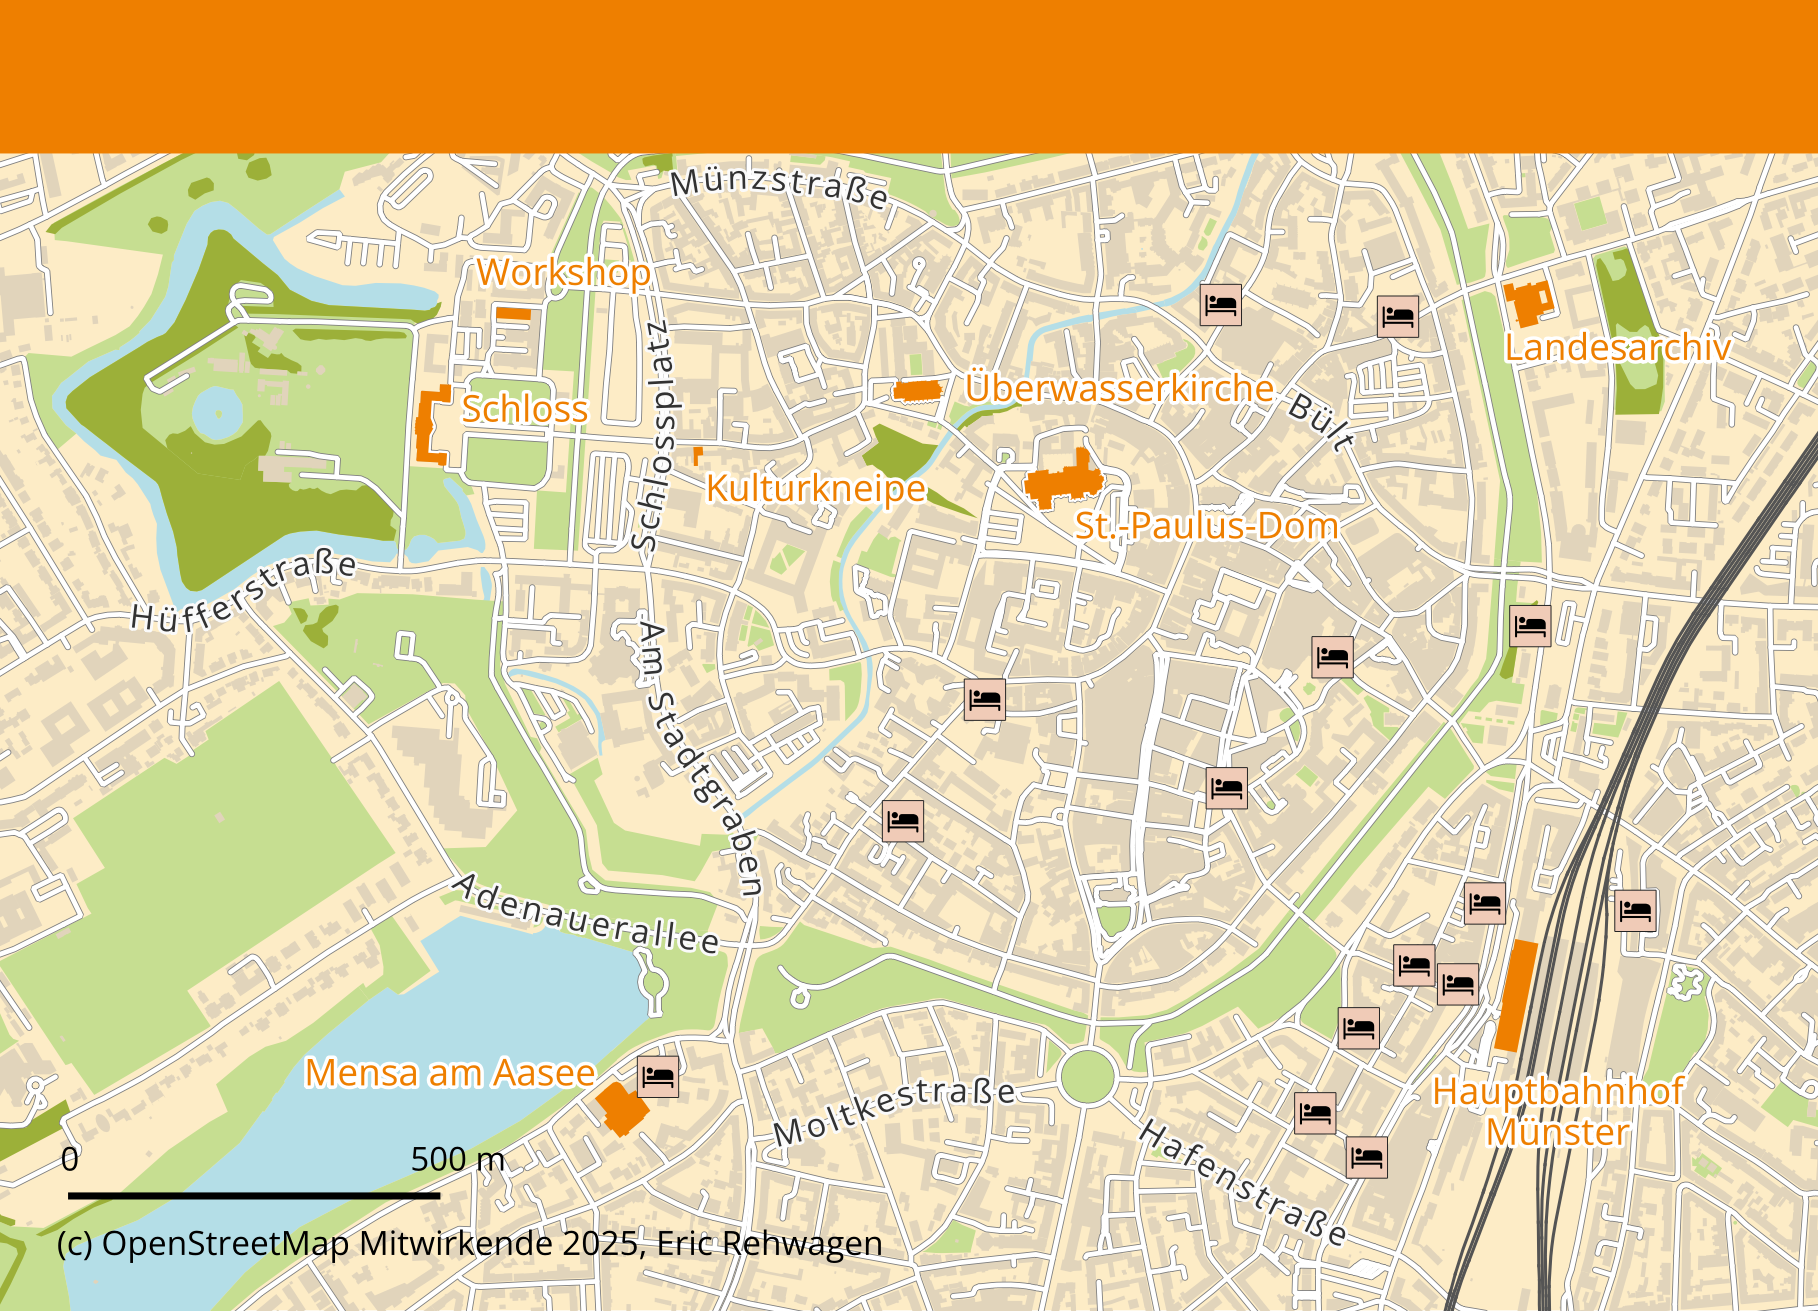
\includegraphics[width=148mm,angle=90,origin=c]{images-print/2025-02-13_Karte_Muenster.png}%
      };%
      \end{tikzpicture}%
   }%
]{uebersicht-alle-haeuser}
\newpairofpagestyles[]{page-uebersicht-alle-haeuser}{}
\AddLayersAtBeginOfPageStyle{page-uebersicht-alle-haeuser}{uebersicht-alle-haeuser}
\AddLayersAtBeginOfPageStyle{page-uebersicht-alle-haeuser}{cropmarksplain}

% Übersicht Räume Schloss Münster
\DeclareNewLayer[background,%
  width=115mm,%
  height=158mm,%
  hoffset=20mm,%
  voffset=10mm,%
  contents={%
    \begin{tikzpicture}[x=1mm, y=1mm]%
      % map image
      \draw (0,0) node [inner sep=0mm, anchor=south west] {%
        \includegraphics[width=148mm,angle=90,origin=c]{images-print/Strichgrafik_Übersicht_schloss_muenster.png}%
      };%
      \end{tikzpicture}%
   }%
]{Schloss_Muenster}
\newpairofpagestyles[]{page-Schloss_Muenster}{}
\AddLayersAtBeginOfPageStyle{page-Schloss_Muenster}{Schloss_Muenster}
\AddLayersAtBeginOfPageStyle{page-Schloss_Muenster}{cropmarksplain}



 
\pagestyle{cropmarksstyle}
\begin{titlepage}
  \thispagestyle{page-title}
  \null
\end{titlepage}
\pagestyle{cropmarksstyle}

\pagenumbering{gobble}\section*{Notizen}

\newpage
\pagenumbering{arabic}
%\setcounter{page}{1}
\section*{Inhalt}
\label{contents}
\newlength\contentspace
\setlength\contentspace{0.2em}

\vspace*{\contentspace}%
\noindent Exkursionen, Abendveranstaltung, Rahmenprogramm  \dotfill \pageref{exkursionen}

\vspace*{\contentspace}%
\noindent Platin- und Goldsponsoren \dotfill \pageref{platinsposoren}

\vspace*{\contentspace}%
\noindent Workshops am Mittwoch \dotfill \pageref{mittwoch-workshops}

\vspace*{\contentspace}%
\noindent Workshops am Donnerstag \dotfill \pageref{donnerstag-workshops}

\vspace*{\contentspace}%
\noindent Workshops am Freitag \dotfill \pageref{freitag-workshops}

\vspace*{\contentspace}%
\noindent Vorträge am Mittwoch \dotfill \pageref{mittwoch}

\vspace*{\contentspace}%
\noindent Vorträge am Donnerstag \dotfill \pageref{donnerstag}

\vspace*{\contentspace}%
\noindent Postersession am Donnerstag \dotfill \pageref{donnerstag-poster}

\vspace*{\contentspace}%
\noindent Vorträge am Freitag \dotfill \pageref{freitag}

\vspace*{\contentspace}%
\noindent OpenStreetMap-Samstag \dotfill \pageref{samstag}

\vspace*{\contentspace}%
\noindent Impressum \dotfill \pageref{impressum}

\vspace*{\contentspace}%
\noindent Medienpartner \dotfill \pageref{medienpartner}

\vspace*{\contentspace}%
\noindent Campusplan und Raumpläne \dotfill \pageref{kartenseiten}

\justifying

\newpage

%\clearpage
%\newpage
\section*{25~Jahre FOSSGIS~e.V. -- Willkommen zur FOSSGIS-Konferenz 2025 in Münster!}\label{welcome}

\begin{flushright}

\includegraphics[width=1.0\textwidth]{Logo_Verein_25.png}
\end{flushright}

\noindent
Im Jahr 2025 wird der FOSSGIS e.V. 25 Jahre alt. Gegründet wurde der Verein als
GRASS Anwendervereinung (GAV e.V.) am 15.04.2000 in Hannover. Über die Zeit
kamen immer mehr Software-Projekte hinzu, weshalb der Verein im Jahr 2008 in
FOSSGIS e.V. umbenannt wurde. {\bfseries  FOSSGIS} steht für {\bfseries f}reie
{\bfseries O}pen"={\bfseries S}ource"={\bfseries S}oftware für
{\bfseries G}eo\-{\bfseries i}nformations\-{\bfseries s}ysteme.
Neben dem Thema \glqq Open-Source-Software\grqq wurde auch das
Thema der offenen Geodaten immer wichtiger. Seit 2017 ist der FOSSGIS~e.V.
auch der offizielle Vertreter des OpenStreetMap-Projektes in Deutschland.

\noindent
Kern unserer Arbeit ist die jährliche FOSSGIS-Konferenz, die Entwickler und
Nutzende zusammenbringt. Wir sind aber auch über die Konferenzen hinaus aktiv,
gehen zu Veranstaltungen, beantworten Fragen in Online-Foren oder betreuen
die digitale Infrastruktur hinter den Projekten.

\pagebreak
\noindent
Die Nachfrage nach Informationen und Vernetzung steigt stetig an. Dies zeigt sich
an den Teilnehmerzahlen der Konferenzen, wie auch an der Zahl der E-Mails und
Telefonanrufe, die uns täglich erreichen. Daher hat der Verein seit fünf Jahren
eine professionelle Koordinierungsstelle, die die ehrenamtliche Arbeit
unterstützt und als Schnittstelle nach Außen dient. Ende 2023 wurde die
Koordinierungsstelle speziell für den OSM-Bereich erweitert.

\noindent
Nach wie vor wird die meiste Arbeit im Verein von Ehrenamtlichen getragen.
Dazu braucht es Menschen, die mitmachen und sich engagieren, Ideen einbringen
und unsere Zukunft mitgestalten wollen. Vielleicht kommen Sie mal am
FOSSGIS-Stand vorbei und reden Sie mit uns! Wir freuen uns auf Ihre Fragen und
Ideen und vielleicht haben Sie ja auch Lust mitzumachen!

\noindent
Die {\bfseries FOSSGIS-Konferenz 2025} wird vom gemeinnützigen FOSSGIS e.V. und der
OpenStreetMap-Community in Kooperation mit dem Institut für Geoinformatik der
Universität Münster veranstaltet. 
Die FOSSGIS-Konferenz ist eine Communityveranstaltung und wird vorwiegend
ehrenamtlich organisiert.
Ziel der Konferenz ist die Verbreitung von freier, quelloffener Software für
Geoinformationssysteme. In den nächsten vier Tagen haben Sie die Gelegenheit,
sich mit Entwickler:innen und anderen Anwender:innen auszutauschen und
neueste Informationen zu Anwendungen und Arbeitsmöglichkeiten zu erhalten.

\pagebreak
\noindent
Konferenzbeiträge zum Vereinsjubiläum:
\begin{description}
\item{\bfseries Mittwoch, 10:30 im Eröffnungsblock:} 25~Jahre FOSSGIS~e.V. - in der Zeitreise durch das Vereinsleben werden verschiedene Mitglieder und Aktive aus dem FOSSGIS~e.V. Aktivitäten, Highlights, Erinnerungen, Erfahrungen, Geschichten aus der Vereinsarbeit teilen.
\item{\bfseries Mittwoch 17:40 - 18:40 \HSeins:} Podiumsgespräch zu 25~Jahre FOSSGIS e.V. - was haben wir geschafft und wo wollen wir hin.
%\item{\bfseries Donnerstag 19:00 \BoFeins:} Mitgliederversammlung des FOSSGIS~e.V. - Gäste sind willkommen.
\item{\bfseries Freitag 15:15 \HSeins:} Ein Blick in die Koordinierungsstelle des FOSSGIS~e.V.
\end{description}

\section*{Exkursionen {\normalfont\em (Anmeldung erforderlich)}}\label{exkursionen}
\noindent
{\large \bfseries Führung durch die Kartensammlung des Landesarchiv NRW}\\
Es wird durch das Magazin des Landesarchiv NRW Abteilung Westfalen geführt. Der Schwerpunkt liegt auf der Kartensammlung und umfasst Karten und Archivgut vom 16. Jahrhundert bis in die Gegenwart. {\bfseries Freitag, 28.03.2025, 17:00} Treffpunkt: Landesarchiv NRW Abteilung Westfalen, Bohlweg 2.
\bigskip

\noindent
{\large \bfseries Archäologisch historischer Stadtrundgang}\\
Vom Domplatz geht es zur Überwasserkirche (dort eine Ausgrabung wegen Fernwärmebau, besonders interessantes Siedlungsgebiet) und weiter zur Jüdefelderstraße. Über den Buddenturm und Zwinger zum Mauritztor von dort aus über den alten Fischmarkt zum Prinzipalmarkt. Auf dem Rundgang werden abgeschlossene und aktuelle Ausgrabungsstellen sowie archäologisches Arbeiten (Vermessungsdaten, Planerstellung, Datenablage etc.) im städtischen Raum vorgestellt. {\bfseries Samstag, 29.03.2025, 14:00~Uhr }, Treffpunkt: S-Bahn Haltestelle Stadthausbrücke, Bahnsteig, Aufgang zur Michaeliskirche.
\bigskip

\section*{Abendveranstaltung am Mittwoch}\label{schwaetzli}
Am ersten Abend der FOSSGIS-Konferenz findet die Abendveranstaltung in der Mensa am Aasee (Bismarckallee~11, 48151~Münster) von {\bfseries 19:00 bis 22:00 Uhr} statt. Eine Anmeldung ist erforderlich.

\section*{Rahmenprogramm am Donnerstag}
\subsection*{Gruppenfoto}
Auch in diesem Jahr wollen wir uns das Gruppenfoto nicht entgehen lassen und laden Sie am {\bfseries Donnerstag} in der {\bfseries Nachmittagspause} zum Gruppenfoto ein am Haupteingang des Schloss Münster.

\subsection*{Mitgliederversammlung des FOSSGIS e.V.}
Am {\bfseries Donnerstag} sind alle Mitglieder und Gäste ab {\bfseries 19.00 Uhr} herzlich zur Mitgliederversammlung des FOSSGIS e.V. eingeladen zum Diskutieren, Kennenlernen und Abstimmen. Ab 18:30 Uhr
gibt es Getränke und Pizza für alle. Der Verein freut sich über zahlreiches Erscheinen.

\section*{Rahmenprogramm am Freitag}

\subsection*{Sektempfang am FOSSGIS-Stand}
Alle Mitglieder des FOSSGIS-Vereins, Freunde und Interessierte sind am {\bfseries Freitag} ab {\bfseries 16.30 Uhr} herzlich zum Sektempfang zum Ausklang der FOSSGIS 2024 am FOSSGIS-Vereins-Stand eingeladen.

\subsection*{OSM-Event am Freitagabend}
Für alle, die am {\bfseries Freitagabend} noch in der Stadt sind und/oder am OSM-Event teilnehmen möchten, wird ein Treffpunkt bekanntgegeben.

\pagebreak
\section*{OSM-Samstag}
Am Samstag, den 29.~März findet von 9.00 bis 17.30~Uhr die OSM-Unkonferenz statt.
Interessierte sind eingeladen sich zu beteiligen oder daran teilzunehmen.
Die Themensammlung erfolgt im OSM-Wiki. Die Veranstaltung ist kostenfrei.
Um Anmeldung über das FOSSGIS-Konferenz-Anmeldesystem wird gebeten.

\subsection*{Community-Sprint}
Beim Community-Sprint wird gemeinsam an OpenSource Projekten gearbeitet.
Die Veranstaltung startet um 9~Uhr mit einem kurzen Vortrag, der für Einsteiger:innen
und Interessierte erklärt wie OpenSource funktioniert und wie man beitragen kann.
Im Anschluss wird gemeinsam oder individuell an Projekten gearbeitet.
Um Anmeldung über das FOSSGIS-Konferenz-Anmeldesystem wird gebeten.

%\clearpage
%\input{workshops}
\section*{Workshops am Mittwoch}\label{mittwoch-workshops}

% time: Wednesday 14:15
% URL: https://pretalx.com/fossgis2023/talk/fossgis2025-57853-einfhrung-geoserver/

\newSmallTimeslot{14:15}
\noindent\workshop{Einführung GeoServer}{Daniel Koch, Nils Bühner}{WS1 (106)}
\workshopspace

%%%%%%%%%%%%%%%%%%%%%%%%%%%%%%%%%%%%%%%%%%%

% time: Wednesday 14:15
% URL: https://pretalx.com/fossgis2023/talk/fossgis2025-56743-mapbender-workshop/


\noindent\workshop{Mapbender Workshop}{Astrid Emde, Thekla Wirkus}{WS2 (107)}
\workshopspace

%%%%%%%%%%%%%%%%%%%%%%%%%%%%%%%%%%%%%%%%%%%

% time: Wednesday 14:15
% URL: https://pretalx.com/fossgis2023/talk/fossgis2025-58115-qgis-workshop/


\noindent\workshop{QGIS Workshop}{Klaus Mithöfer, Thomas Piribauer}{WS3 (108)}
\workshopspace

%%%%%%%%%%%%%%%%%%%%%%%%%%%%%%%%%%%%%%%%%%%

% time: Wednesday 16:30
% URL: https://pretalx.com/fossgis2023/talk/fossgis2025-57815-postgresql-postgis-workshop-fr-einsteiger/

\newSmallTimeslot{16:30}
\noindent\workshop{PostgreSQL / PostGIS Workshop für Einsteiger}{Jörg Thomsen, Annika Fröde}{WS1 (106)}
\workshopspace

%%%%%%%%%%%%%%%%%%%%%%%%%%%%%%%%%%%%%%%%%%%

% time: Wednesday 16:30
% URL: https://pretalx.com/fossgis2023/talk/fossgis2025-58051-datenschutz-und-geografische-informationen/


\noindent\workshop{Datenschutz und geografische Informationen}{Falk Zscheile}{WS2 (107)}
\workshopspace

%%%%%%%%%%%%%%%%%%%%%%%%%%%%%%%%%%%%%%%%%%%

% time: Wednesday 16:30
% URL: https://pretalx.com/fossgis2023/talk/fossgis2025-57863-hands-on-masterportal-erweiterte-konfiguration/


\noindent\workshop{Hands on Masterportal: Erweiterte Konfiguration}{Hannes Blitza}{WS3 (108)}
\workshopspace

%%%%%%%%%%%%%%%%%%%%%%%%%%%%%%%%%%%%%%%%%%%

\vspace*{-1.5cm}
\section*{Workshops am Donnerstag}\label{donnerstag-workshops}

% time: Thursday 09:00
% URL: https://pretalx.com/fossgis2023/talk/fossgis2025-58291-geodatenverarbeitung-mit-triggern-und-views-im-geopackage/

\newSmallTimeslot{09:00}
\noindent\workshop{Geodatenverarbeitung mit Triggern und Views im Geopackage}{Claas Leiner}{WS1 (106)}
\workshopspace

%%%%%%%%%%%%%%%%%%%%%%%%%%%%%%%%%%%%%%%%%%%

% time: Thursday 09:00
% URL: https://pretalx.com/fossgis2023/talk/fossgis2025-58124-erstellen-von-bi-dashboards-mit-apache-superset/


\noindent\workshop{Erstellen von BI-Dashboards mit Apache Superset}{Jan Suleiman, Daniel Koch}{WS2 (107)}
\workshopspace

%%%%%%%%%%%%%%%%%%%%%%%%%%%%%%%%%%%%%%%%%%%

% time: Thursday 09:00
% URL: https://pretalx.com/fossgis2023/talk/fossgis2025-57712-automatisierung-von-qgis-workflows-mit-eigenen-verarbeitungswerkzeugen/


\noindent\workshop{Automatisierung von QGIS-Workflows mit eigenen Verarbeitungswerkzeugen}{Peter Gipper, Johannes Kröger}{WS3 (108)}
\workshopspace

%%%%%%%%%%%%%%%%%%%%%%%%%%%%%%%%%%%%%%%%%%%

% time: Thursday 11:10
% URL: https://pretalx.com/fossgis2023/talk/fossgis2025-57850-orchestrierung-einer-gdi-ber-container-images/

\newSmallTimeslot{11:10}
\noindent\workshop{Orchestrierung einer GDI über Container Images}{Daniel Koch, Nils Bühner}{WS1 (106)}
\workshopspace

%%%%%%%%%%%%%%%%%%%%%%%%%%%%%%%%%%%%%%%%%%%

% time: Thursday 11:10
% URL: https://pretalx.com/fossgis2023/talk/fossgis2025-58055-hands-on-qgis-js-interaktive-qgis-basierte-webkarten-erstellen/


\noindent\workshop{Hands-on qgis-js: Interaktive QGIS-basierte Webkarten erstellen}{Michael Schmuki}{WS2 (107)}
\workshopspace

%%%%%%%%%%%%%%%%%%%%%%%%%%%%%%%%%%%%%%%%%%%

% time: Thursday 11:10
% URL: https://pretalx.com/fossgis2023/talk/fossgis2025-58256-wie-kann-ich-mit-python-ein-qgis-plugin-programmieren-/


\noindent\workshop{Wie kann ich mit Python ein QGIS-Plugin programmieren?}{Isabelle Korsch}{WS3 (108)}
\workshopspace

%%%%%%%%%%%%%%%%%%%%%%%%%%%%%%%%%%%%%%%%%%%

% time: Thursday 14:15
% URL: https://pretalx.com/fossgis2023/talk/fossgis2025-58664-qgis-programmierung-ohne-python-vorkenntnisse/

\newSmallTimeslot{14:15}
\noindent\workshop{QGIS-Programmierung ohne Python-Vorkenntnisse}{Numa Gremling}{WS1 (106)}
\workshopspace

%%%%%%%%%%%%%%%%%%%%%%%%%%%%%%%%%%%%%%%%%%%

% time: Thursday 14:15
% URL: https://pretalx.com/fossgis2023/talk/fossgis2025-58213-einfaches-geodatenmanagement-mit-geonetwork-und-geonetwork-ui/


\noindent\workshop{Einfaches Geodatenmanagement mit\linebreak GeoNetwork und GeoNetwork-UI}{Angelika Kinas, Olivia Guyot}{WS2 (107)}
\workshopspace

%%%%%%%%%%%%%%%%%%%%%%%%%%%%%%%%%%%%%%%%%%%

% time: Thursday 14:15
% URL: https://pretalx.com/fossgis2023/talk/fossgis2025-58251-kartierung-von-berflutungsgebieten-aus-sentinel-1-radardaten-mit-hilfe-von-actinia/


\noindent\workshop{Kartierung von Überflutungsgebieten aus Sentinel-1 Radardaten mit Hilfe von actinia}{Markus Metz, Carmen Tawalika, Markus Neteler}{WS3 (108)}
\workshopspace

%%%%%%%%%%%%%%%%%%%%%%%%%%%%%%%%%%%%%%%%%%%

% time: Thursday 16:45
% URL: https://pretalx.com/fossgis2023/talk/fossgis2025-57865-mapproxy-workshop-optimierung-und-beschleunigung-von-web-map-services/

\newSmallTimeslot{16:45}
\noindent\workshop{MapProxy Workshop~-- Optimierung und Beschleunigung von Web Map Services}{Hannes Blitza}{WS1 (106)}
\workshopspace

%%%%%%%%%%%%%%%%%%%%%%%%%%%%%%%%%%%%%%%%%%%

% time: Thursday 16:45
% URL: https://pretalx.com/fossgis2023/talk/fossgis2025-58052-die-open-database-license-odbl-erklrt/


\noindent\workshop{Die Open Database License (ODbL) erklärt}{Falk Zscheile}{WS2 (107)}
\workshopspace

%%%%%%%%%%%%%%%%%%%%%%%%%%%%%%%%%%%%%%%%%%%

% time: Thursday 16:45
% URL: https://pretalx.com/fossgis2023/talk/fossgis2025-58111-offline-webanwendung-pwa-mit-cloud-optimierten-vectortiles/


\noindent\workshop{Offline Webanwendung (PWA) mit cloud-optimierten Vectortiles}{Eva-Marie Schürg, Marwin Ludwig}{WS3 (108)}
\workshopspace

%%%%%%%%%%%%%%%%%%%%%%%%%%%%%%%%%%%%%%%%%%%

\section*{Workshops am Freitag}\label{freitag-workshops}

% time: Friday 09:00
% URL: https://pretalx.com/fossgis2023/talk/fossgis2025-58234-mergin-maps-essentials/

\newSmallTimeslot{09:00}
\noindent\workshop{Mergin Maps Essentials}{Peter Petrik}{WS2 (107)}
\workshopspace

%%%%%%%%%%%%%%%%%%%%%%%%%%%%%%%%%%%%%%%%%%%

% time: Friday 09:00
% URL: https://pretalx.com/fossgis2023/talk/fossgis2025-58242-eoc-eo-products-service-zugriff-und-nutzung-von-geodaten-mit-stac/


\noindent\workshop{EOC EO Products Service~-- Zugriff und Nutzung von Geodaten mit STAC}{Felix Feckler}{WS3 (108)}
\workshopspace

%%%%%%%%%%%%%%%%%%%%%%%%%%%%%%%%%%%%%%%%%%%

% time: Friday 11:10
% URL: https://pretalx.com/fossgis2023/talk/fossgis2025-58088-qfield-in-der-praxis-feldarbeit-leicht-gemacht/

\newSmallTimeslot{11:10}
\noindent\workshop{QField in der Praxis~-- Feldarbeit leicht gemacht}{Berit Mohr, Michael Schmuki}{WS1 (106)}
\workshopspace

%%%%%%%%%%%%%%%%%%%%%%%%%%%%%%%%%%%%%%%%%%%

% time: Friday 11:10
% URL: https://pretalx.com/fossgis2023/talk/fossgis2025-58252-osm-transform-leistungsstarke-osm-datenvorbereitung-fr-routing-engines/


\noindent\workshop{OSM-Transform —  Leistungsstarke OSM-Datenvorbereitung für Routing Engines}{Julian Psotta, Jakob Schnell, Till Frankenbach}{WS2 (107)}
\workshopspace

%%%%%%%%%%%%%%%%%%%%%%%%%%%%%%%%%%%%%%%%%%%

% time: Friday 11:10
% URL: https://pretalx.com/fossgis2023/talk/fossgis2025-60277-interaktive-karten-mit-openlayers/


\noindent\workshop{Interaktive Karten mit OpenLayers}{Andreas Hocevar}{WS3 (108)}
\workshopspace

%%%%%%%%%%%%%%%%%%%%%%%%%%%%%%%%%%%%%%%%%%%

\cleardoubleevenpage
%\newpage
%\enlargethispage{0.0\baselineskip}
\renewcommand{\arraystretch}{1.4}
\section*{Vorträge am Mittwoch}\label{mittwoch}
\renewcommand{\conferenceDay}{\mittwoch}
\setPageBackground
\noindent\begin{tabular}{Z{0.7cm}Z{6.85cm}}
  & \multicolumn{1}{c}{\HSeins}
  \tabularnewline
  10:00
  \talk{Eröffnung}{FOSSGIS e.V.}
  \tabularnewline
  10:10
  \talk{Keynote und Begrüßung}{Josef Hovenjuergen}
  \tabularnewline
 10:30
  \talk{25. Jahre FOSSGIS e.V. - eine Zeitreise durch das Vereinsleben}{Katja Haferkorn, Maik S., Christopher Lorenz}
  \tabularnewline
\end{tabular}

\noindent\begin{tabular}{Z{0.7cm}Z{3.0cm}Z{3.0cm}}
  & \multicolumn{1}{c}{\HSeins}
  & \multicolumn{1}{c}{\HSzwei}
  \tabularnewline
11:45
  \talk{Eine Reise durch die Geoportale Deutschlands}{Matthias Mohr}
  \talk{spatial.IO - Cloud-basierte Open-Source-Lösung zur Verwaltung räumlicher Daten}{Rebekka Lange}
  \tabularnewline
  12:20
  \talk{GIS-Schulprojekte in Zusammenarbeit mit kommunalen Gebietskörperschaften}{
Dietmar Holzner}
  \talk{eoAPI - eine skalierbare Geodateninfrastruktur}{
Felix Delattre}
  \tabularnewline
 \rowcolor{commongray}
 12:45 & \multicolumn{2}{c}{%
   \parbox[c]{24pt}{%
     \includegraphics[height=10pt]{restaurant}%
   }
   Mittagspause
} \tabularnewline
\end{tabular}
%
%\vspace{0.5\baselineskip}

\noindent\begin{tabular}{Z{0.7cm}Z{3.0cm}Z{3.0cm}}
  & \multicolumn{1}{c}{\HSdrei}
  & \multicolumn{1}{c}{\HSvier}
  \tabularnewline
  11:45
  \talk{GeoPandas - als Tool zur Basiskartenaktualisierung}{Markus Albrecht, Markus Gruber}
  \talk{Keine Angst vor der GeoInfoDok 7 - 3A-Datenverarbeitung mit PostNAS}{Oliver Schmidt}
  \tabularnewline
  12:20
  \talk{aviary - ein generisches Python-Framework zur KI-Inferenz für Fernerkundungsdate}{Marius Maryniak}
  \talk{GDI per Knopfdruck: Automatisierung mit DevOps und Infrastruktur als Code}{Jakob Miksch}
  \tabularnewline
  \rowcolor{commongray}
  12:45 & \multicolumn{2}{c}{%
    \parbox[c]{24pt}{%
      \includegraphics[height=10pt]{restaurant}%
    }
    Mittagspause
  } \tabularnewline
\end{tabular}

\noindent\begin{tabular}{Z{0.7cm}Z{3.0cm}Z{3.0cm}}
  & \multicolumn{1}{c}{\HSeins}
  & \multicolumn{1}{c}{\HSzwei}
\tabularnewline
  14:15
  \talk{basemap.de als Open Data - Neue Stile und Anwendungsbeispiel}{Arnulf B. Bichler (aka Christl)}
  \talk{Automatischer Import und Veröffentlichung von Betriebsmittelgeometrien mittels PyQGIS}{Philipp Opitz}
 \tabularnewline
  14:50
  \talk{Open Data in D: Perfekte Idee, halbherzige Umsetzung? Ein Erfahrungsbericht.}{Mike Elstermann}
\talk{QGIS-Werkzeuge und Python}{Isabelle Korsch}
  \tabularnewline
  15:25
 \talk{Open Data des BKG (II)}{Joachim Eisenberg}
  \talk{Schnupperkurs: Das Potential von QGIS mit der Python-Konsole freischalten}{Gordon Schlolaut}
    \tabularnewline
  \rowcolor{commongray}
  16:00 & \multicolumn{2}{c}{%
    \parbox[c]{24pt}{%
      \includegraphics[height=10pt]{cafe}%
    }
    Kaffeepause \emph{(30 min)}}
   \tabularnewline
\end{tabular}
\newpage

\renewcommand{\arraystretch}{1.4}
\noindent\begin{tabular}{Z{0.7cm}Z{3.0cm}Z{3.0cm}}
  & \multicolumn{1}{c}{\HSdrei}
  & \multicolumn{1}{c}{\HSvier}
  \tabularnewline
  14:15
  \talk{Superset - Business Intelligence meets Cartography}{Jan Suleiman}
  \talk{Lightning-Talks}{}
  \tabularnewline
  14:50
  \talk{Visualisierung von historischen Schiffsrouten mit unscharfer Datengrundlage}{Stefan Fuest, Andreas Gollenstede, Jennifer Tadge, Maximilian Herbers, Rieke Marie Kaiser}
  \talk{Wie MapLibre und Vektorkarten die Welt übernehmen}{Bart Louwers, Just van den Broecke}
    \tabularnewline
  15:25
  \talk{Automatisierte Verarbeitung von Daten der Meeresbodenkartografie mit QGIS}{Helge Staedtler}
  \talk{Vektor Tiles für Karten mit Echtzeitdaten}{Pirmin Kalberer}
  \tabularnewline
%  \rowcolor{commongray}
%  16:00 & \multicolumn{2}{c}{%
%   \parbox[c]{24pt}{%
%      \includegraphics[height=10pt]{cafe}%
%   }
%    Kaffeepause
% } \tabularnewline
\end{tabular}

%\subsubsection*{Anwendertreffen und Demo-Sessions am Mittwoch}%\label{demomittwoch}
\label{demomittwoch}
\renewcommand{\arraystretch}{1.4}
   \enlargethispage{10\baselineskip}
\justifying\setPageBackground

\noindent\begin{tabular}{Z{0.7cm}Z{2.0cm}Z{2.0cm}Z{2.0cm}}
  & \multicolumn{1}{c}{\BoFeins}
  & \multicolumn{1}{c}{\BoFzwei}
  & \multicolumn{1}{c}{\BoFdrei}
  \tabularnewline
14:15
  \talk{Studierende stellen ihre Arbeit vor \emph{(60min)}}{}
  \talk{BoF GeoNode-DE \emph{(60min)}}{Matthes Rieke, Henning Bredel}
  \talk{Lizmap Webclient \emph{(60min)}}{Günter Wagner}
  \tabularnewline
%  \rowcolor{commongray}
% 16:00 & \multicolumn{3}{c}{%
 %   \parbox[c]{24pt}{%
 %     \includegraphics[height=10pt]{cafe}%
%    }
%    Kaffeepause
%  } \tabularnewline
  \end{tabular}

\noindent\begin{tabular}{Z{0.7cm}Z{3.0cm}Z{3.0cm}}
  & \multicolumn{1}{c}{\HSeins}
  & \multicolumn{1}{c}{\HSzwei}
\tabularnewline
  16:30
     \talk{Small seeds - FOSS Communitys stärken!}{Paul Robben}
  \talk{Von Proprietär zu QGIS}{David Arndt}
  \tabularnewline
  17:05
  \talk{Governance von Open-Source-Software im öffentlichen Sektor: Make, Buy or Contribute?}{Christian Weidner}
  \talk{Von proprietär zu Open-Source -Umstellung der kommunalen GDI bei der Stadt Reutlingen}{Simon Kondic}
    \tabularnewline
  17:40
  \longTalk{2}{Panelgespräch: 25 Jahre FOSSGIS e.V. - was haben wir geschafft und wo wollen wir hin}{Torsten Friebe, David Arndt, Torsten Wiebke}
  \talk{Migration eines Auskunftssystems zu einer Open-Source Lösung mit QGIS}{Victor Ali Lagoa}
  \tabularnewline
  18:15
  \talk{}{}
%\talk{Projekt GEOrg bei den SWM: Mit Freier Software zur konzernweiten Geodatenplattform}{Nina Röckelein, Benedikt Seidl}
\talk{Projekt GEOrg bei den SWM: Mit Freier Software zur konzernweiten Geodatenplattform}{N. Röckelein, B. Seidl}
   \tabularnewline
\end{tabular}

\small
\noindent\begin{tabular}{Z{0.7cm}Z{6.0cm}}
  & \multicolumn{1}{c}{\BoFzwei}
  \tabularnewline
16:30
  \talk{Open Geodata und Open Source GIS Software in den Kultur- und Geisteswissenschaften \emph{(60min)}}{Anastasia Bauch, Carmen M. Enss, Klaus Stein}
\tabularnewline
  \end{tabular}
\normalsize

\newpage

\vspace{0.5\baselineskip}
\enlargethispage{4.0\baselineskip}
\renewcommand{\arraystretch}{1.4}
\renewcommand{\baselinestretch}{1.1}

\vspace{0.5\baselineskip}
%\enlargethispage{1.0\baselineskip}

\noindent\begin{tabular}{Z{0.7cm}Z{3.0cm}Z{3.0cm}}
  & \multicolumn{1}{c}{\HSdrei}
  & \multicolumn{1}{c}{\HSvier}
  \tabularnewline
  16:30
  \talk{Die Leistungsfähigkeit großer open source Sprachmodelle für Geoparsing-Aufgaben}{Juiwen Chang (Ariel)}
  \talk{Open ALKIS? – Oder was passiert, wenn der deutsche Föderalismus auf EU-Recht trifft}{Stefan Zaunseder}
  \tabularnewline
  17:05
  \talk{Entwicklung eines LLM-basierten Assistenten für die Suche nach Geodaten}{Matthes Rieke, Simeon Wetzel}
  \talk{Was wäre, wenn wir Algorithmen demokratisieren? Kollaborative Infrastrukturen für UDZ}{Rico H. Herzog}
  \tabularnewline
  17:40
  \talk{Künstliche Intelligenz als Unterstützung in geografische Applikationen}{Andrea Borghi, Marion Baumgartner}
  \talk{Metadaten für eine verantwortungsvolle und kritische Geodatenpraxis}{Ester Scheck}
  \tabularnewline
 18:15
  \talk{Open Data und KI im Einsatz: Geodaten für alle, nicht nur für Profis?}{Lisa Stubert, Klemens Maget}
  \talk{MOSIDI - Homogenisierung von offenen Daten für die kommunale Planung}{Sebastian Meier}
 %\tabularnewline
  \end{tabular}
  
\label{endevortraegemittwoch}
\renewcommand{\arraystretch}{1.4}
%\justifying\setPageBackground  
\newpage


% time: Wednesday 10:00
% URL: https://pretalx.com/fossgis2023/talk/fossgis2025-59156-erffnung/

%
\newTimeslot{10:00}
\noindent\abstractHSeins{%
  %
}{%
  Eröffnung%
}{%
}{%
  Feierliche Eröffnung der Konferenz durch Vertreter des FOSSGIS~e.V. mit Hinweisen zum
  Ablauf und der Organisation.%
}%


%%%%%%%%%%%%%%%%%%%%%%%%%%%%%%%%%%%%%%%%%%%

% time: Wednesday 10:10
% URL: https://pretalx.com/fossgis2023/talk/fossgis2025-65632-keynote-und-begrung/

%
\newSmallTimeslot{10:10}
\noindent\abstractHSeins{%
  Josef Hovenjuergen%
}{%
  Keynote und Begrüßung%
}{%
}{%
  Begrüßungsworte und Keynotebeitrag des parlamentarischen Staatssekretärs im Ministerium für Heimat, Kommunales, Bau und Digitalisierung
  des Landes Nordrhein-Westfalen, Josef Hovenjuergen.%
}%


%%%%%%%%%%%%%%%%%%%%%%%%%%%%%%%%%%%%%%%%%%%

% time: Wednesday 10:30
% URL: https://pretalx.com/fossgis2023/talk/fossgis2025-57803-25-jahre-fossgis-e-v-eine-zeitreise-durch-das-vereinsleben/

%
\newSmallTimeslot{10:30}
\noindent\abstractHSeins{%
  Katja Haferkorn, Maik S., Christopher Lorenz%
}{%
  25. Jahre FOSSGIS e.V.~-- eine Zeitreise durch das Vereinsleben%
}{%
}{%
  Die AG-25 hat sich überlegt einen Vortragsblock für den Eröffnungsblock zu organisieren, in dem
  einige Mitglieder Erinnerungen, Erfahrungen oder Highlights aus der Vereinsarbeit teilen.
  Angelehnt ans Lightningtalk-Format wird ein Feuerwerk aus 25 Jahren FOSSGIS~e.V. gezündet,
  untermalt mit Geschichten, Bildern und Fotos.%
}%


%%%%%%%%%%%%%%%%%%%%%%%%%%%%%%%%%%%%%%%%%%%

% time: Wednesday 11:45
% URL: https://pretalx.com/fossgis2023/talk/fossgis2025-58249-eine-reise-durch-die-geoportale-deutschlands/

%
\newTimeslot{11:45}
\noindent\abstractHSeins{%
  Matthias Mohr%
}{%
  Eine Reise durch die Geoportale Deutschlands%
}{%
}{%
  Im letzten Jahr musste ich Datensätze für Feldgrenzen in Deutschland finden. Was erst einmal
  einfach klingt endete mit einer Odyssee durch die verschiedensten Geoportale der Länder. Ich nehme
  euch auf dieser Reise mit und beschreibe, was mir bei der Reise aufgefallen ist und wie man diese
  Erfahrung in der Praxis verbessern könnte.%
}%


%%%%%%%%%%%%%%%%%%%%%%%%%%%%%%%%%%%%%%%%%%%

% time: Wednesday 11:45
% URL: https://pretalx.com/fossgis2023/talk/fossgis2025-58113-spatial-io-cloud-basierte-open-source-lsung-zur-verwaltung-rumlicher-daten/

%

\noindent\abstractHSzwei{%
  Rebekka Lange%
}{%
  spatial.IO~-- Cloud-basierte Open-Source-Lösung zur Verwaltung räumlicher Daten%
}{%
}{%
  Mit zunehmenden Datenmengen im Bereich der Umweltsystemforschung steigt die Notwendigkeit für
  geeignete Dateninfrastrukturen zur automatisierten Verwaltung und Repräsentation der Daten. In
  diesem Vortrag stellen wir die Open-Source-Lösung
  spatial.IO des Helmholtz-Zentrums für
  Umweltforschung (UFZ) vor, welche unabhängig von bestehenden IT-Infrastrukturen überall betrieben
  werden kann.%
}%

\pagebreak
%%%%%%%%%%%%%%%%%%%%%%%%%%%%%%%%%%%%%%%%%%%

% time: Wednesday 11:45
% URL: https://pretalx.com/fossgis2023/talk/fossgis2025-58166-geopandas-als-tool-zur-basiskartenaktualisierung/

%

\noindent\abstractHSdrei{%
  Markus Gruber, Markus Albrecht%
}{%
  GeoPandas~-- als Tool zur Basiskarten\-aktualisierung%
}{%
}{%
  Die Grundlagenkarte der Stadtwerke München ist eine Sammlung von Daten aus verschiedenen Quellen
  wie amtlichen Daten und eigenen Erhebungen. Sie umfasst ca. 14.000 km² und wird mit PostGIS
  verwaltet. 2024 wurden die ETL-Prozesse auf eine Open Source Lösung basierend auf Python und
  GeoPandas migriert, um die Flexibilität und Performance zu erhöhen. Die Transformationen werden
  auf einem Kubernetes-Cluster ausgeführt, wodurch der Import von mehreren Tagen auf 6 Stunden
  reduziert werden konnte.%
}%


%%%%%%%%%%%%%%%%%%%%%%%%%%%%%%%%%%%%%%%%%%%

% time: Wednesday 11:45
% URL: https://pretalx.com/fossgis2023/talk/fossgis2025-57049-keine-angst-vor-der-geoinfodok-7-3a-datenverarbeitung-mit-postnas/

%

\noindent\abstractHSvier{%
  Oliver Schmidt%
}{%
  Keine Angst vor der GeoInfoDok 7~-- 3A-Datenverarbeitung mit PostNAS%
}{%
}{%
  Für viele Andwendungen müssen 3A-Daten im Format der GeoInfoDok 7.1.2 verarbeitet werden. Vor dem
  Hintergrund der Open\-Data-Bereitstellung des LVermGeo Rheinland-Pfalz steigt nun auch das Interesse
  an originären 3A-Daten und an AdV-konformen WFS und WMS.
  Import- und Verarbeitungsschritte, mit denen 3A-Daten in eine PostGIS-Datenbank überführt werden,
  sind Teil dieses Vortrages. Ebenso werden eigene Skripte und hieraus erzeugte Geowebdienste
  vorgestellt.%
}%


%%%%%%%%%%%%%%%%%%%%%%%%%%%%%%%%%%%%%%%%%%%

% time: Wednesday 12:20
% URL: https://pretalx.com/fossgis2023/talk/fossgis2025-58280-gis-schulprojekte-in-zusammenarbeit-mit-kommunalen-gebietskrperschaften/

%
\newTimeslot{12:20}
\noindent\abstractHSeins{%
  Dietmar Holzner%
}{%
  GIS-Schulprojekte in Zusammenarbeit mit kommunalen Gebietskörperschaften%
}{%
}{%
  Zusammenarbeit zwischen einem technischen Gymnasium und den umliegenden kommunalen Körperschaften
  zur georeferenzierten Erfassung von Infrastrukturen. Im Rahmen eines einwöchigen
  Vermessungspraktikums vermessen Schüler/innen die Objekte und erfassen sie in einer
  georeferenzierten Datenbank. Grafische Darstellung und Datenhandling erfolgt mittels QGIS durch
  die Verbindung mit der Datenbank.%
}%


%%%%%%%%%%%%%%%%%%%%%%%%%%%%%%%%%%%%%%%%%%%

% time: Wednesday 12:20
% URL: https://pretalx.com/fossgis2023/talk/fossgis2025-57279-eoapi-eine-skalierbare-geodateninfrastruktur/

%

\noindent\abstractHSzwei{%
  Felix Delattre%
}{%
  eoAPI~-- eine skalierbare Geodaten\-infrastruktur%
}{%
}{%
  In diesem Vortrag geht es um eoAPI, ein Open-Source-Baukasten zur schnellen Bereitstellung einer
  skalierbaren Geodaten\-infra\-struktur auf Grundlage der STAC-Spezifikation. eoAPI ermöglicht die
  einfache Auffindbarkeit und breite Nutzung von Erdbeobachtungsdaten. Es werden ihre
  leistungsstarken Funktionen sowie die Komponenten TiTiler, Tipg, pgSTAC und stac-fastapi
  erläutert.%
}%

\pagebreak
%%%%%%%%%%%%%%%%%%%%%%%%%%%%%%%%%%%%%%%%%%%

% time: Wednesday 12:20
% URL: https://pretalx.com/fossgis2023/talk/fossgis2025-58285-aviary-ein-generisches-python-framework-zur-ki-inferenz-fr-fernerkundungsdaten/

%

\noindent\abstractHSdrei{%
  Marius Maryniak%
}{%
  aviary~-- ein generisches Python-Framework zur KI-Inferenz für Fernerkundungsdaten%
}{%
}{%
  aviary ist ein generisches Python-Framework, das die Inferenz von KI-Modellen für
  Fernerkundungsdaten vereinfacht.
  Es bietet verschiedene Pipelines mit austauschbaren, erweiterbaren Komponenten. Neben der Nutzung
  als Python-Package können vorgefertigte Pipelines über die Kommandozeile verwendet werden.
  Künftig sollen vortrainierte Modelle für diverse Anwendungsfälle sowie
  speziell auf Fernerkundungsdaten trainierte Foundation-Modelle bereitgestellt werden.%
}%


%%%%%%%%%%%%%%%%%%%%%%%%%%%%%%%%%%%%%%%%%%%

% time: Wednesday 12:20
% URL: https://pretalx.com/fossgis2023/talk/fossgis2025-57638-gdi-per-knopfdruck-automatisierung-mit-devops-und-infrastruktur-als-code/

%

\noindent\abstractHSvier{%
  Jakob Miksch%
}{%
  GDI per Knopfdruck: Automatisierung mit DevOps und Infrastruktur als Code%
}{%
}{%
  Der Vortrag zeigt auf wie eine Geodateninfrastruktur(GDI) automatisiert über Code eingerichtet
  werden kann und geht dabei auf die von uns genutzten Software-Bausteine und deren Alternativen
  ein.%
}%


%%%%%%%%%%%%%%%%%%%%%%%%%%%%%%%%%%%%%%%%%%%

% time: Wednesday 14:15
% URL: https://pretalx.com/fossgis2023/talk/fossgis2025-58266-basemap-de-als-open-data-neue-stile-und-anwendungsbeispiele/

%
\newTimeslot{14:15}
\noindent\abstractHSeins{%
  Arnulf B. Bichler (aka Christl)%
}{%
  basemap.de als Open Data~-- Neue Stile und Anwendungsbeispiele%
}{%
}{%
  Die Grundlage der basemap.de sind amtliche Daten der Länder, die seit Mitte 2024 als Open Data
  bereitgestellt werden. In dem Vortrag werden neue Möglichkeiten gezeigt, die sich daraus ergeben
  und neue Stile vorgestellt. In Anwendungsbeispielen werden die Potenziale für Behörden und eigene
  Entwicklungen gezeigt.%
}%


%%%%%%%%%%%%%%%%%%%%%%%%%%%%%%%%%%%%%%%%%%%

% time: Wednesday 14:15
% URL: https://pretalx.com/fossgis2023/talk/fossgis2025-57703-automatischer-import-und-verffentlichung-von-betriebsmittelgeometrien-mittels-pyqgis/

%

\noindent\abstractHSzwei{%
  Philipp Opitz%
}{%
  Automatischer Import und Veröffent\-lichung von Betriebsmittelgeometrien mittels PyQGIS%
}{%
}{%
  Ziel von Versorgungsunternehmen ist ein minimaler Zeitraum zwischen Beendingung einer Baumaßnahme
  und Integration der Geodaten in die Leitungsauskunft. Eine Möglichkeit bietet die automatische
  Integration der Geometrien als Vorabauskunft. In der Umsetzung bei SachsenEnergie wurde für die
  Datenveröffentlichung ein ETL-Prozess auf QGIS/PyQGIS-Basis entwickelt, welcher differenziell und
  performant nächtlich die DXF-Daten in eine Datenbank überführt. Die Publikation der Daten erfolgt
  mittels WMS.%
}%


%%%%%%%%%%%%%%%%%%%%%%%%%%%%%%%%%%%%%%%%%%%

% time: Wednesday 14:15
% URL: https://pretalx.com/fossgis2023/talk/fossgis2025-58092-superset-business-intelligence-meets-cartography/

%

\noindent\abstractHSdrei{%
  Jan Suleiman%
}{%
  Superset~-- Business Intelligence meets Cartography%
}{%
}{%
  Superset ist eine der meistgenutzten Open-Source Tools im Bereich der Business Intelligence (BI).
  Wir haben Superset um die Erstellung thematischer Karten erweitert, wodurch auch raum-zeitliche
  Aspekte besser analysiert werden können. In diesem Vortrag zeigen wir, wie sowohl Kartodiagramme,
  Choroplethenkarten, sowie Proportional Symbol Maps in Superset erstellt und für raum-zeitliche
  Analysen verwendet werden können.%
}%

\newLightningTimeslot{14:15}
%%%%%%%%%%%%%%%%%%%%%%%%%%%%%%%%%%%%%%%%%%%

% time: Wednesday 14:15
% URL: https://pretalx.com/fossgis2023/talk/fossgis2025-57772-foss-basierte-schnittstelle-zum-management-von-heritage-bim-modellen/

%

\noindent\abstractHSvier{%
  Güren Tan Dinga, Laura Fernandez Resta%
}{%
  FOSS-basierte Schnittstelle zum\linebreak Management von Heritage BIM Modellen%
}{%
}{%
  Die Integration von Heritage BIM in die Erhaltung historischer Gebäude ist insbesondere bei der
  zukünftigen Bewirtschaftung dieser von hoher Relevanz. Am Beispiel des UNESCO-Welterbes
  Speicherstadt Hamburg wurde eine benutzerorientierte Schnittstelle entwickelt, welche es
  Nutzer:innen ohne BIM-Kenntnisse ermöglicht, Zugang zu strukturierten Gebäudeinformationen zu
  gewähren. Dafür wurden offene Standards wie IFC und FOSS genutzt, wodurch die Interoperabilität
  und Kollaboration gefördert wurden.%
}%


%%%%%%%%%%%%%%%%%%%%%%%%%%%%%%%%%%%%%%%%%%%

% time: Wednesday 14:20
% URL: https://pretalx.com/fossgis2023/talk/fossgis2025-57804-amtliche-orthofotos-zentral-verfgbar-eine-open-source-lsung-fr-deutschland/

%

\newLightningTimeslot{14:20}
\noindent\abstractHSvier{%
  Moritz Lucas%
}{%
  Amtliche Orthofotos zentral verfügbar: Eine Open-Source-Lösung für Deutschland%
}{%
}{%
  In Deutschland werden amtliche Orthophotos mittlerweile in allen Bundesländern frei zugänglich
  bereitgestellt, geregelt durch die INSPIRE-Richtlinie. Doch die föderale Struktur führt zu 16
  unterschiedlichen Diensten, die den Zugriff auf diese hochwertigen Bilddaten erschweren. Die
  vorgestellte Software bietet eine zentrale Lösung, die den deutschlandweiten Download vereinfacht.
  Ziel ist es, mehr Aufmerksamkeit für Orthophotos zu schaffen und deren Nutzung sowie
  Weiterentwicklung zu fördern.%
}%


%%%%%%%%%%%%%%%%%%%%%%%%%%%%%%%%%%%%%%%%%%%

% time: Wednesday 14:25
% URL: https://pretalx.com/fossgis2023/talk/fossgis2025-59167-ergebnisprsentation-des-code-sprints/

%

\newLightningTimeslot{14:25}
\noindent\abstractHSvier{%
  %
}{%
  Ergebnispräsentation des Code-Sprints%
}{%
}{%
  In diesem doppelten Lightning-Talk-Block werden im Schnelldurchlauf die Ergebnisse des bereits
  seit Anfang der Woche stattfindenden Code-Sprints präsentiert.%
}%

%\vspace{0.5cm}
\sponsorBoxA{402_mundialis.png}{0.37\textwidth}{5}{%
\textbf{Bronzesponsor und Aussteller}\\
\noindent\small {\bfseries mundialis GmbH \& Co. KG} mundialis ist spezialisiert auf die Auswertung und Verarbeitung von Fernerkundungs- und Geodaten mit dem Schwerpunkt Cloud-basierte Geoprozessierung. Wir setzen Freie \& Open Source Geoinformationssysteme (GRASS GIS, actinia, QGIS, u.a.) ein, mit denen wir maßgeschneiderte Lösungen für den Kunden entwickeln.
\normalsize
}%


\newTimeslot{14:15}
\enlargethispage{1.8\baselineskip}
%%%%%%%%%%%%%%%%%%%%%%%%%%%%%%%%%%%%%%%%%%%

% time: Wednesday 14:15
% URL: https://pretalx.com/fossgis2023/talk/fossgis2025-63518-studierende-stellen-ihre-arbeit-vor/

%

\noindent\abstractAnwBoFeins{%
  %
}{%
  Studierende stellen ihre Arbeit vor%
}{%
}{%
  Studierende stellen Ihre Arbeit vor (Masterarbeit, Bachelorarbeit, aktuell in Arbeit,
  Seminararbeit, Praktikumsaufgaben, Abschlussarbeiten(Ausbildung) .%
}%


%%%%%%%%%%%%%%%%%%%%%%%%%%%%%%%%%%%%%%%%%%%

% time: Wednesday 14:15
% URL: https://pretalx.com/fossgis2023/talk/fossgis2025-57854-bof-geonode-de/

%

\noindent\abstractAnwBoFzwei{%
  Henning Bredel, Matthes Rieke%
}{%
  BoF GeoNode-DE%
}{%
}{%
  Die Gruppe GeoNode-DE möchte gemeinsam Fragen zur Weiterentwicklung diskutieren und das vorhandene
  Netzwerk zu stärken.%
}%


%%%%%%%%%%%%%%%%%%%%%%%%%%%%%%%%%%%%%%%%%%%

% time: Wednesday 14:15
% URL: https://pretalx.com/fossgis2023/talk/fossgis2025-58049-lizmap-webclient/

%

\noindent\abstractAnwBoFdrei{%
  Günter Wagner%
}{%
  Lizmap Webclient%
}{%
}{%
  Diese Fragestunde, kombiniert mit Demo-Beispielen, ermöglicht Interessierten einen Einblick in den
  Webclient Lizmap in Kombination mit dem QGIS-Server. Neben den Fragen der Teilnehmer werden
  spezielle Funktionen und Neuerungen vorgestellt. Dabei ist die Expert:innenfragestunde sowohl für
  neu interessierte als auch für Anwender vom Lizmap Webclient interessant.%
}%
\sponsorBoxA{403_grit.png}{0.16\textwidth}{2}{%
\textbf{Bronzesponsor}\\
\noindent\small Die {\bfseries grit GmbH} ist ein Software- und Beratungsunternehmen im Bereich der Geo-IT mit Standorten in Werne und Olpe. Die Kernkompetenzen sind Geoinformationssysteme und Geodateninfrastrukturen, wobei vorzugsweise Open Source-Technologien in containerisierten Umgebungen zum Einsatz kommen.
\normalsize
}%


%%%%%%%%%%%%%%%%%%%%%%%%%%%%%%%%%%%%%%%%%%%

% time: Wednesday 14:50
% URL: https://pretalx.com/fossgis2023/talk/fossgis2025-58131-open-data-in-d-perfekte-idee-halbherzige-umsetzung-ein-erfahrungsbericht-/

%
\newTimeslot{14:50}
\noindent\abstractHSeins{%
  Mike Elstermann%
}{%
  Open Data in D: Perfekte Idee, halbherzige Umsetzung? Ein Erfahrungsbericht.%
}{%
}{%
  Open Data ist gut, aber nur, wenn ...
  Lange haben wir sie gefordert und darum gekämpft und zum Glück gibt es sie jetzt, diese deutschen
  offenen Geobasisdaten, in allen Bundesländern, aber mit unterschiedlicher Ausprägung. Mein
  persönlicher Erfahrungsbericht soll den aktuellen Status und das Verbesserungspotenzial zeigen und
  zur Diskussion zwischen Nutzern und Anbietern anregen .%
}%


%%%%%%%%%%%%%%%%%%%%%%%%%%%%%%%%%%%%%%%%%%%

% time: Wednesday 14:50
% URL: https://pretalx.com/fossgis2023/talk/fossgis2025-58278-qgis-werkzeuge-und-python/

%

\noindent\abstractHSzwei{%
  Isabelle Korsch%
}{%
  QGIS-Werkzeuge und Python%
}{%
}{%
  Mit Python kann der Funktionsumfang von QGIS erweitert werden, aber es muss nicht immer ein
  QGIS-Plugin sein: Häufig lohnt es sich auch mit Python neue Werkzeuge in QGIS zu erstellen. Wie
  funktioniert das?%
}%

\sponsorBoxA{404_opencage-logo.png}{0.4\textwidth}{4}{%
\textbf{Bronzesponsor}\\
\noindent\small {\bfseries OpenCage GmbH} aus Hannover bietet eine auf offenen Daten basierende Geokodierung API (forward und reverse geocoding). Sei es einmalige Datenverarbeitung, Systemintegration oder maßgeschneiderte highly-available Systeme für Millionen Anfragen am Tag. Wir organisieren Geomob Tech Talks und Podcast.
\normalsize
}%


\pagebreak
%%%%%%%%%%%%%%%%%%%%%%%%%%%%%%%%%%%%%%%%%%%

% time: Wednesday 14:50
% URL: https://pretalx.com/fossgis2023/talk/fossgis2025-57948-visualisierung-von-historischen-schiffsrouten-mit-unscharfer-datengrundlage/

%

\noindent\abstractHSdrei{%
  Stefan Fuest, Andreas Gollenstede, Jennifer Tadge, Maximilian Herbers, Rieke Marie Kaiser%
}{%
  Visualisierung von historischen Schiffs\-routen mit unscharfer Datengrundlage%
}{%
}{%
  Im Forschungsverbund DiViAS (www.divias.de) werden Quellen wie Logbücher und Journale aus dem
  18./19. Jh. ausgewertet und analysiert. Im Fokus dieses Vortrags stehen dabei verschiedene
  Möglichkeiten der Visualisierung von Schiffsrouten mit unscharfer Datengrundlage, welche mit QGIS
  und Mapbox erstellt werden. Grundlage für die kartographische Darstellung ist eine KI-gestützte
  Extraktion von unscharfen Orts- und Zeitangaben aus diesen Quellen und deren Modellierung in einer
  PostgreSQL-Datenbank.%
}%


%%%%%%%%%%%%%%%%%%%%%%%%%%%%%%%%%%%%%%%%%%%

% time: Wednesday 14:50
% URL: https://pretalx.com/fossgis2023/talk/fossgis2025-58293-wie-maplibre-und-vektorkarten-die-welt-bernehmen/

%

\noindent\abstractHSvier{%
  Bart Louwers, Just van den Broecke%
}{%
  Wie MapLibre und Vektorkarten die Welt übernehmen%
}{%
}{%
  Vektorbasierte Karten sind die Zukunft! Oder vielleicht sogar schon die Gegenwart? In diesem
  Vortrag werden beide Perspektiven beleuchtet! Bart spricht aus der Perspektive der Entwicklung von
  MapLibre, und gibt einen Einblick in den neuesten Stand. Just erzählt von seinen Erfahrungen als
  Benutzer der MapLibre-Stack um vektorbasierte Karten zu gestalten.%
}%


%%%%%%%%%%%%%%%%%%%%%%%%%%%%%%%%%%%%%%%%%%%

% time: Wednesday 15:25
% URL: https://pretalx.com/fossgis2023/talk/fossgis2025-58227-open-data-des-bkg-ii-/

%
\newTimeslot{15:25}
\noindent\abstractHSeins{%
  Joachim Eisenberg%
}{%
  Open Data des BKG (II)%
}{%
}{%
  Das Bundesamt für Kartographie und Geodäsie (BKG) hat ein breites Open Data-Angebot, das auf der
  letzten FOSSGIS-Konferenz in Hamburg vorgestellt wurde. Was hat sich mit der Umsetzung der
  HVD-Verordnung an diesem Angebot getan?%
}%


%%%%%%%%%%%%%%%%%%%%%%%%%%%%%%%%%%%%%%%%%%%

% time: Wednesday 15:25
% URL: https://pretalx.com/fossgis2023/talk/fossgis2025-58127-schnupperkurs-das-potential-von-qgis-mit-der-python-konsole-freischalten/

%

\noindent\abstractHSzwei{%
  Gordon Schlolaut%
}{%
  Schnupperkurs: Das Potential von QGIS mit der Python-Konsole freischalten%
}{%
}{%
  Programmierung mit Python ermöglicht es, sich eigene Werkzeuge in QGIS zu erstellen und so den
  Funktionsumfang von QGIS individuell zu erweitern und den eigenen Bedürfnissen anzupassen. Aber
  wie funktioniert das alles eigentlich und womit fängt man an? Dieser Vortrag gibt einen kurzen und
  verständlichen Überblick auch für alle ohne Programmier-Vorkenntnisse. Wir werden live ein kleines
  Werkzeug schreiben, an dem wir die grundlegenden Konzepte vorstellen und zeigen: es ist gar nicht
  so schwierig.%
}%
\sponsorBoxA{405_GBD.png}{0.35\textwidth}{2}{%
\textbf{Bronzesponsor und Aussteller}\\
\noindent\small Die {\bfseries Geoinformatikbüro Dassau GmbH} aus Düsseldorf bietet seit 2006 Beratung, Konzeption, Schulung, Wartung, Support und Programmierung zum Thema GIS und GDI auf Open Source Basis. Ein Fokus liegt auf der Software QGIS, QGIS Server, QField, QGIS Web Client, GBD WebSuite, PostgreSQL/PostGIS und GRASS GIS.
\normalsize
}%

\pagebreak
%%%%%%%%%%%%%%%%%%%%%%%%%%%%%%%%%%%%%%%%%%%

% time: Wednesday 15:25
% URL: https://pretalx.com/fossgis2023/talk/fossgis2025-58269-automatisierte-verarbeitung-von-daten-der-meeresbodenkartografie-mit-qgis/

%

\noindent\abstractHSdrei{%
  Helge Staedtler%
}{%
  Automatisierte Verarbeitung von Daten der Meeresbodenkartografie mit QGIS%
}{%
}{%
  Es wird ein Einblick gegeben wie Rasterdaten mit Hilfe genannter GIS Open Source Werkzeuge \&
  Dienste automatisiert verarbeitet werden können. Im unternehmerischen Kontext beschäftige ich mich
  gemeinsam im Team mit hyperspektralen und RGB Unterwasserdaten, und deren ML-unterstützter
  Verarbeitung, um den Meeresboden zu analysieren \& zu kartografieren. Für die Verarbeitung werden
  Werkzeuge wie z.B. GDAL, QGIS, OSM und \LaTeX\  eingesetzt.%
}%


%%%%%%%%%%%%%%%%%%%%%%%%%%%%%%%%%%%%%%%%%%%

% time: Wednesday 15:25
% URL: https://pretalx.com/fossgis2023/talk/fossgis2025-58089-vektor-tiles-fr-karten-mit-echtzeitdaten/

%

\noindent\abstractHSvier{%
  Pirmin Kalberer%
}{%
  Vektor Tiles für Karten mit Echtzeitdaten%
}{%
}{%
  Vektorkacheln sind eine effiziente Art, um Karten mit grossen Mengen an Echtzeitdaten
  bereitzustellen.%
}%

\sponsorBoxA{407_geoSYS_logo.png}{0.35\textwidth}{4}{%
\textbf{Bronzesponsor und Aussteller}\\
\noindent\small {\bfseries geoSYS} ist Dienstleister im Bereich Geoinformation. Wir beraten Unternehmen, Verwaltungen bei der Einführung von GIS, Geodatenbanken, Geodateninfrastrukturen und Webmapping-Lösungen. Wir entwickeln Anwendungen, Portale, Geo-Apps und auch GIS-Plugins und setzen Projekte in aller Welt um.
\normalsize
}%

%%%%%%%%%%%%%%%%%%%%%%%%%%%%%%%%%%%%%%%%%%%

% time: Wednesday 16:30
% URL: https://pretalx.com/fossgis2023/talk/fossgis2025-57856-small-seeds-foss-communities-strken-/

%
\newTimeslot{16:30}
\noindent\abstractHSeins{%
  Paul Robben%
}{%
  Small seeds~-- FOSS Communities stärken!%
}{%
}{%
  Mehr finanzielle Mittel für Freie und Open-Source-Software~-- die unendliche Geschichte. In einer
  von Start-ups, VC Funding und datensammelnden Apps geprägten Tech-Welt ist der Kampf um
  nachhaltige Finanzierungen für ethische Technologieprojekte besonders hart. Nach einigen großen
  Erfolgen für die Förderung von FOSS in den letzten Jahren geht es in diesem Vortrag nun darum, die
  kleinen, weniger sichtbaren zivilgesellschaftlichen Projekte nicht zu vergessen.%
}%


%%%%%%%%%%%%%%%%%%%%%%%%%%%%%%%%%%%%%%%%%%%

% time: Wednesday 16:30
% URL: https://pretalx.com/fossgis2023/talk/fossgis2025-57851-von-proprietr-zu-qgis/

%

\noindent\abstractHSzwei{%
  David Arndt%
}{%
  Von Proprietär zu QGIS%
}{%
}{%
  QGIS erfreut sich einer großen Beliebtheit. Der Regionalverband Ruhr setzt QGIS schon seit einiger
  Zeit als Standard GIS-System ein. In diesem Vortrag sollen die Erfahrungen geteilt werden wie ein
  Umstieg von ArcGIS erfolgen kann. Dabei werden Aspekte wie Kosten, Features, Einbindung in eine
  vorhandene GDI betrachtet.%
}%

\pagebreak
%%%%%%%%%%%%%%%%%%%%%%%%%%%%%%%%%%%%%%%%%%%

% time: Wednesday 16:30
% URL: https://pretalx.com/fossgis2023/talk/fossgis2025-58126-die-leistungsfhigkeit-groer-open-source-sprachmodelle-fr-geoparsing-aufgaben/

%

\noindent\abstractHSdrei{%
  Juiwen Chang (Ariel)%
}{%
  Die Leistungsfähigkeit großer open source Sprachmodelle für Geoparsing-Aufgaben%
}{%
}{%
  Wir präsentieren einen Geoparsing-Workflow, der Name Entity Recognition und Geokodierung
  kombiniert, um Ortsangaben inklusive Hausnummern aus Texten zu extrahieren und in einem WebGIS zu
  visualisieren. Wir haben moderne großer Sprachmodelle (LLM) wie Meta Llama3.1-70b-instruct und
  Mistral-large getestet und dabei herausgefunden, dass ein hybrider Open-Source-Ansatz bis
  zu 70 \% der Standorte korrekt erkennt~-- womit der Ansatz besser ist als Anthropic Claude und
  ChatGPT o1-preview.%
}%


%%%%%%%%%%%%%%%%%%%%%%%%%%%%%%%%%%%%%%%%%%%

% time: Wednesday 16:30
% URL: https://pretalx.com/fossgis2023/talk/fossgis2025-58192-open-alkis-oder-was-passiert-wenn-der-deutsche-fderalismus-auf-eu-recht-trifft/

%

\noindent\abstractHSvier{%
  Stefan Zaunseder%
}{%
  Open ALKIS?~-- Oder was passiert, wenn der deutsche Föderalismus auf EU-Recht trifft%
}{%
}{%
  Wir befinden uns im Jahr 2024. Die Durchführungsverordnung (EU) 2023/138 tritt in Kraft und sorgt
  dafür, dass wesentliche Teile des Liegenschaftskatasters als Open Data zur Verfügung stehen. Das
  gilt auch in Deutschland für ALKIS. Doch hier sind die Bundesländer zuständig, was zu einem
  Sammelsurium von Umsetzungen führt. Und ein von unbeugsamen Bajuwaren bevölkertes Land hört nicht
  auf, den Europäern Widerstand zu leisten. Das Leben ist nicht leicht für Open Data-Enthusiasten...%
}%

\pagebreak
%%%%%%%%%%%%%%%%%%%%%%%%%%%%%%%%%%%%%%%%%%%

% time: Wednesday 16:30
% URL: https://pretalx.com/fossgis2023/talk/fossgis2025-63538-studierende-stellen-ihre-arbeit-vor/

%

\noindent\abstractAnwBoFeins{%
  %
}{%
  Studierende stellen ihre Arbeit vor%
}{%
}{%
  Studierende stellen Ihre Arbeit vor (Masterarbeit, Bachelorarbeit, aktuell in Arbeit,
  Seminararbeit, Praktikumsaufgaben, Abschlussarbeiten(Ausbildung) .%
}%


%%%%%%%%%%%%%%%%%%%%%%%%%%%%%%%%%%%%%%%%%%%

% time: Wednesday 16:30
% URL: https://pretalx.com/fossgis2023/talk/fossgis2025-58071-open-geodata-und-open-source-gis-software-in-den-kultur-und-geisteswissenschaften/

%

\noindent\abstractAnwBoFzwei{%
  Klaus Stein, Carmen M. Enss, Anastasia Bauch%
}{%
  Open Geodata und Open Source GIS Software in den Kultur- und Geisteswissenschaften%
}{%
}{%
  Vernetzungstreffen für alle, die Open Source GIS Software in den Kultur- und Geisteswissenschaften
  einsetzen (wollen), an offenen Geodaten arbeiten, oder an diesen Themen Interesse haben.%
}%

\sponsorBoxA{408_MerginMaps.png}{0.34\textwidth}{2}{%
\textbf{Bronzesponsor und Aussteller}\\
\noindent\small {\bfseries Mergin Maps} ist ein auf QGIS basierendes Tool zur Felddatenerfassung, mit dem Sie Daten erfassen, speichern und mit Ihrem Team synchronisieren können. Sie können Ihre QGIS-Projekte in die mobile App übertragen, Daten erfassen und diese wieder auf dem Server synchronisieren.
\normalsize
}%

%%%%%%%%%%%%%%%%%%%%%%%%%%%%%%%%%%%%%%%%%%%

% time: Wednesday 17:05
% URL: https://pretalx.com/fossgis2023/talk/fossgis2025-58262-governance-von-open-source-software-im-ffentlichen-sektor-make-buy-or-contribute-/

%
\newTimeslot{17:05}
\noindent\abstractHSeins{%
  Christian Weidner%
}{%
  Governance von Open-Source-Software im öffentlichen Sektor: Make, Buy or\linebreak Contribute?%
}{%
}{%
  Die Governance von OSS im öffentlichen Sektor variiert stark: Während einige Projekte offen und
  kollaborativ sind, bleiben andere hierarchisch strukturiert. Dieser Beitrag untersucht, warum
  Behörden sich für oder gegen die Öffnung ihrer Softwareprojekte entscheiden. Die Untersuchung gibt
  Einblick in ausgewählte OSS-Projekte der öffentlichen Verwaltung und liefert einen
  Erklärungsansatz, warum Faktoren wie Unsicherheit, Innovationsdruck und normative Erwartungen die
  Entscheidung beeinflussen.%
}%


%%%%%%%%%%%%%%%%%%%%%%%%%%%%%%%%%%%%%%%%%%%

% time: Wednesday 17:05
% URL: https://pretalx.com/fossgis2023/talk/fossgis2025-58190-von-proprietr-zu-open-source-umstellung-der-kommunalen-gdi-bei-der-stadt-reutlingen/

%

\noindent\abstractHSzwei{%
  Simon Kondic, Linus Lambrecht%
}{%
  Von proprietär zu Open-Source -Umstellung der kommunalen GDI bei der Stadt Reutlingen%
}{%
}{%
  Die Stadt Reutlingen, eine Großstadt in Baden-Württemberg, stellte ihre kommunale
  Geodateninfrastruktur (GDI) von proprietärer auf Open-Source Software um. Ziel ist eine größere
  digitale Souveränität, Lizenzkostenreduktion und Unabhängigkeit von kommerziellen Anbietern. Im
  Vortrag wird die Vorgehensweise der Systemmigration und der Aufbau der neuen Open-Source GDI
  vorgestellt.%
}%


%%%%%%%%%%%%%%%%%%%%%%%%%%%%%%%%%%%%%%%%%%%

% time: Wednesday 17:05
% URL: https://pretalx.com/fossgis2023/talk/fossgis2025-58109-entwicklung-eines-llm-basierten-assistenten-fr-die-suche-nach-geodaten/

%

\noindent\abstractHSdrei{%
  Simeon Wetzel, Matthes Rieke%
}{%
  Entwicklung eines LLM-basierten\linebreak Assistenten für die Suche nach Geodaten%
}{%
}{%
  Unser Vortrag stellt ein innovatives Framework zur Verbesserung der Geodatensuche vor. Durch die
  Kombination von Large Language Models, dialogbasierter Nutzerinteraktion und semantischer Suche
  sollen die Limitierungen traditioneller, metadatenbasierter Suchsysteme überwunden werden. Das
  System ermöglicht eine präzisere Erfassung von Nutzeranforderungen und kann sowohl Metadaten als
  auch die eigentlichen Geodatenattribute durchsuchen, was die Qualität der Suchergebnisse deutlich
  verbessert.%
}%


%%%%%%%%%%%%%%%%%%%%%%%%%%%%%%%%%%%%%%%%%%%

% time: Wednesday 17:05
% URL: https://pretalx.com/fossgis2023/talk/fossgis2025-58130-was-wre-wenn-wir-algorithmen-demokratisieren-kollaborative-infrastrukturen-fr-udz/

%

\noindent\abstractHSvier{%
  Rico H Herzog%
}{%
  Was wäre, wenn wir Algorithmen demokratisieren? Kollaborative Infrastrukturen für UDZ%
}{%
}{%
  Das Paper zeigt, wie neue kollaborative Infrastrukturen für Urbane Digitale Zwillinge eine bessere
  Teilhabe und Zugang zur Simulationsentwicklung schaffen können. Am Beispiel von drei
  Open-Source-Tools aus dem "`Connected Urban Twins"-Projekt wird demonstriert, wie Szenarien für
  Stadtentwicklungsprozesse gemeinsam entwickelt, analysiert und zugänglich gemacht werden können.
  Ziel ist eine nachhaltigere, inklusivere Planung, die durch vielfältige Perspektiven blinde
  Flecken in Modellen reduziert.%
}%


%%%%%%%%%%%%%%%%%%%%%%%%%%%%%%%%%%%%%%%%%%%

% time: Wednesday 17:40
% URL: https://pretalx.com/fossgis2023/talk/fossgis2025-58038-25-jahre-fossgis-e-v-was-haben-wir-geschafft-und-wo-wollen-wir-hin/

%
\newTimeslot{17:40}
\noindent\abstractHSeins{%
  Torsten Friebe, David Arndt, Torsten Wiebke%
}{%
  25 Jahre FOSSGIS e.V.~-- was haben wir geschafft und wo wollen wir hin%
}{%
}{%
  Seit Juni 2021 beschäftigt sich die Arbeitsgruppe \glqq Öffentliche Ausschreibungen mit FOSS\grqq\  des
  FOSSGIS~e.V. mit dem Thema der
  Beschaffung und Vergabe von IT-Lösungen auf Basis von FOSS. In dieser Dialogrunde wollen wir mit
  Vertreter:innen des FOSSGIS-Community über die Erfahrungen aus 25 Jahren Einsatz von Open Source
  Software in der öffentlichen Verwaltung diskutieren.%
}%


%%%%%%%%%%%%%%%%%%%%%%%%%%%%%%%%%%%%%%%%%%%

% time: Wednesday 17:40
% URL: https://pretalx.com/fossgis2023/talk/fossgis2025-57890-migration-eines-auskunftssystems-zu-einer-open-source-lsung-mit-qgis/

%

\noindent\abstractHSzwei{%
  Victor Ali Lagoa%
}{%
  Migration eines Auskunftssystems zu einer Open-Source Lösung mit QGIS%
}{%
}{%
  Die Geodatenabteilung der Stadtwerke München nutzte GE Smallworld für ihr Netzinformationssystem,
  was aufgrund steigender Komplexität und Nutzerzahl zu hohen Kosten führte. Vor fünf Jahren begann
  die Migration zu NIS-QGIS, einer kostensparenden, auf QGIS-Desktop und PyQGIS-Plugins basierenden
  Open-Source-Lösung. Der Vortrag liefert einen Überblick über die neue Anwendung, Anwendungsfälle,
  Herausforderungen und Erkenntnisse.%
}%

\pagebreak
%%%%%%%%%%%%%%%%%%%%%%%%%%%%%%%%%%%%%%%%%%%

% time: Wednesday 17:40
% URL: https://pretalx.com/fossgis2023/talk/fossgis2025-58175-knstliche-intelligenz-als-untersttzung-in-geografische-applikationen/

%

\noindent\abstractHSdrei{%
  Marion Baumgartner, Andrea Borghi%
}{%
  Künstliche Intelligenz als Unterstützung in geografische Applikationen%
}{%
}{%
  In dieser Präsentation zeigen wir die Ergebnisse von zwei POCs, welche wir mit dem Large Language
  Models (LLM) Open Source Python Framework "`LangChain” durchgeführt haben. Mittels LLM (wie GPT)
  zeigen wir, wie eine geographische Anwendung durch künstliche Intelligenz benutzerfreundlicher und
  zugänglicher wird. Auch im Hintergrund arbeiten wir mit künstlicher Intelligenz, um die
  Anreicherung und die Indexierung von Metadaten zu verbessern und zu automatisieren.%
}%


%%%%%%%%%%%%%%%%%%%%%%%%%%%%%%%%%%%%%%%%%%%

% time: Wednesday 17:40
% URL: https://pretalx.com/fossgis2023/talk/fossgis2025-57509-metadaten-fr-eine-verantwortungsvolle-und-kritische-geodatenpraxis/

%

\noindent\abstractHSvier{%
  Ester Scheck%
}{%
  Metadaten für eine verantwortungsvolle und kritische Geodatenpraxis%
}{%
}{%
  Die Open Data Bewegung ermöglicht den Zugang zu zahlreichen offenen Datensätzen. Allerdings fehlen
  oft detailliertere Metadaten, die den Kontext der Daten, wie Erhebungsmethoden oder Entscheidungen
  zu Klassifikationen, erklären. Für eine verantwortungsvolle und kritische Geodatenpraxis ist es
  jedoch essentiell, diesen Entstehungskontext einzubeziehen. Ansatzpunkte dafür können Frameworks
  zur Dokumentation und Reflexion des Datenkontextes sowie Metadaten Standards sein.%
}%


%%%%%%%%%%%%%%%%%%%%%%%%%%%%%%%%%%%%%%%%%%%

% time: Wednesday 18:15
% URL: https://pretalx.com/fossgis2023/talk/fossgis2025-57825-projekt-georg-bei-den-swm-mit-freier-software-zur-konzernweiten-geodatenplattform/

%
\newTimeslot{18:15}
\noindent\abstractHSzwei{%
  Nina Röckelein, Benedikt Seidl%
}{%
  Projekt GEOrg bei den SWM: Mit Freier Software zur konzernweiten Geodatenplattform%
}{%
}{%
  Mit freier Software aus dem QGIS-Universum bauen wir bei den Stadtwerken München eine konzernweite
  Geodatenplattform. Wir erzählen von unseren Erfahrungen bei der Integration verschiedener
  Anwendungen und der Etablierung von Open-Source Lösungen im Unternehmen.%
}%


%%%%%%%%%%%%%%%%%%%%%%%%%%%%%%%%%%%%%%%%%%%

% time: Wednesday 18:15
% URL: https://pretalx.com/fossgis2023/talk/fossgis2025-57193-open-data-und-ki-im-einsatz-geodaten-fr-alle-nicht-nur-fr-profis-/

%

\noindent\abstractHSdrei{%
  Klemens Maget, Lisa Stubert%
}{%
  Open Data und KI im Einsatz: Geodaten für alle, nicht nur für Profis?%
}{%
}{%
  Im Rahmen der aktuellen Diskussion zur Nutzung von KI-Sprach\-modellen untersuchen wir in einem
  Proof of Concept, wie KI im Zusammenspiel mit offenen Geodaten eingesetzt werden kann. Kann KI
  dabei unterstützen, frei verfügbare Daten besser aufzufinden, verständlicher zu machen, ihre
  Relevanz für spezifische Projekte zu bewerten oder ganz neue Ideen zu entwickeln? Oder eröffnet
  sie gar die Möglichkeit, neue Nutzendengruppen außerhalb der traditionellen
  Geodaten-Expert:innenkreise anzusprechen?%
}%

\newpage
\enlargethispage{3.0\baselineskip}
%%%%%%%%%%%%%%%%%%%%%%%%%%%%%%%%%%%%%%%%%%%

% time: Wednesday 18:15
% URL: https://pretalx.com/fossgis2023/talk/fossgis2025-58059-mosidi-homogenisierung-von-offenen-daten-fr-die-kommunale-planung/

%
\enlargethispage{3.0\baselineskip}
\noindent\abstractHSvier{%
  Sebastian Meier, Leonard Higi%
}{%
  MOSIDI~-- Homogenisierung von offenen Daten  für die kommunale Planung%
}{%
}{%
  Im Rahmen des Projekts InNoWest wird ein homogenisiertes Datenschema für die kommunale Verwaltung
  entwickelt. Ziel ist es, heterogene räumliche Daten aus öffentlichen und Non-Profit-Quellen zu
  aggregieren und über ein niedrigschwelliges Benutzerinterface bereitzustellen. Durch die
  nutzerzentrierte Entwicklung, abgestimmt auf reale Bedürfnisse brandenburgischer Kommunen, können
  Daten flexibel kombiniert und neue Erkenntnisse für Planung und Daseinsvorsorge generiert werden.%
}%


%%%%%%%%%%%%%%%%%%%%%%%%%%%%%%%%%%%%%%%%%%%

\vspace{-0.2cm}
\sponsorBoxA{202_EFTAS_Slogan.png}{0.4\textwidth}{4}{%
\textbf{Silbersponsor und Aussteller}
\vspace{0.5\baselineskip}

\noindent {\bfseries EFTAS Fernerkundung Technologietransfer GmbH}\\
{\bfseries GeoIT rund um Luft- und Satellitenbilder!}  
Mit Geodaten können wir die Welt besser verstehen.
Deshalb entwickeln wir passgenaue GeoIT-Lösungen, die präzise sind und aktiv die Zukunft
gestalten. Dafür nutzen wir KI und Cloud-Compuing und erstellen individuelle,
technologieoffene Lösungen aus einer Hand, unabhängig von Software- und Datenprovidern.    
{\bfseries Unsere Anwendungswelten:}
\begin{itemize}
\item Land- \& Forstwirtschaft  
\item Umwelt, Natur \& Landschaft  
\item Stadt \& Verkehr  
\ietm Bergbau \& Georessourcen
\end{itemize}
{\bfseries Unser Fokus:}\\ 
Fernerkundung auf Basis von Luft- und Satellitenbildern, die großflächige Erfassung von In-
situ-Daten \& individuelle GeoIT-Anwendungen.   
{\bfseries Unser Ziel:}\\
Umweltrelevante Prozesse und Entscheidungen unterstützen \& beschleunigen - und zwar
weltweit.

\normalsize
}%


\clearpage
\cleardoubleevenpage
%\newpage
%\enlargethispage{0.0\baselineskip}
\renewcommand{\arraystretch}{1.4}
\section*{Vorträge am Donnerstag}\label{donnerstag}
\renewcommand{\conferenceDay}{\donnerstag}
\setPageBackground
\noindent\begin{tabular}{Z{0.7cm}Z{3.0cm}Z{3.0cm}}
  & \multicolumn{1}{c}{\HSeins}
  & \multicolumn{1}{c}{\HSzwei}
  \tabularnewline
 09:00
  \talk{Der Digitale Zwilling - so wertvoll wie eine Karte im Maßstab 1:1}{Matthias Daues}
  \talk{Routing, aber mehr explorativ statt automatisch}{Katharina Rasch}
  \tabularnewline
 09:35
  \talk{Der Wuppertaler Weg vom Geoportal zum Digitalen Zwilling}{Stefan Sander}
  \talk{Flexibles Open Source Routing mit Valhalla}{Christian Beiwinkel}
  \tabularnewline
  10:00
  \talk{Masterportal - Liegenschaftsauskunft ONLIKA 4.0 mit Keycloak und BundID}{Laura Meierkort}
  \talk{Transitous - Freies Public Transport Routing}{Volker Krause}
  \tabularnewline
  \rowcolor{commongray}
  10:25 & \multicolumn{2}{c}{%
    \parbox[c]{24pt}{%
      \includegraphics[height=10pt]{cafe}%
    }
    Frühstückspause~/~Postersession \emph{(35 min)}
  } \tabularnewline
\end{tabular}
%
\newpage
\enlargethispage{3.0\baselineskip}

\vspace*{-1.0\baselineskip}

\noindent\begin{tabular}{Z{0.7cm}Z{3.0cm}Z{3.0cm}}
  & \multicolumn{1}{c}{\HSdrei}
  & \multicolumn{1}{c}{\HSvier}
  \tabularnewline
  09:00
  \talk{Anreicherung von Straßendaten mittels Deep-Learning-Methoden und Mapillary Bildern}{Benjamin Herfort, Sukanya Randhawa}
  \talk{G3W-SUITE: das OS-Framework für die Veröffentlichung und Verwaltung von QGIS-Projekten}{Walter Lorenzetti,\linebreak Antonello Andrea}
  \tabularnewline
  09:35
  \talk{Versiegelungsanalyse zur bioklimatischen Bewertung von Stadtgebieten}{M. Metz, A. Weinmann, M. Eichhorn, V.-L. Brunn}
  \longTalk{2}{Historische Karten mit QGIS georeferenzieren \emph{(45 min)}}{Niklas Alt, Johannes Wagner}
  \tabularnewline
  10:00
  \talk{Ermittlung von versiegelten Flächen als komplexe Aufgabe (Projekt SEAL)}{Peter Lorkowski}
  \talk{}{}
  \tabularnewline
\end{tabular}
\vspace{0.5\baselineskip}

\noindent\begin{tabular}{Z{0.7cm}Z{3.0cm}Z{3.0cm}}
  & \multicolumn{1}{c}{\BoFeins}
  & \multicolumn{1}{c}{\BoFdrei}
  \tabularnewline
09:00
  \talk{Kartographie mit QGIS \emph{(60 min)}}{Andreas Neumann, Mathias Gröbe}
  \talk{OpenStreetMap für und mit öffentlicher Verwaltung und Behörden \emph{(60 min)}}{Lars Lingner,\linebreak Christopher Lorenz}
  \tabularnewline
  \end{tabular}


\noindent\begin{tabular}{Z{0.7cm}Z{3.0cm}Z{3.0cm}}
  & \multicolumn{1}{c}{\HSeins}
  & \multicolumn{1}{c}{\HSzwei}
\tabularnewline
  11:10
  \talk{FOSSGIS bei OpenCode.de}{David Arndt}
  \talk{Barrierefreies Routing mit MOTIS}{Felix Gündling}
 \tabularnewline
  11:45
  \talk{XPlanung mit Open Source Software}{Torsten Friebe}
\talk{Online-Karten für die Verkehrswende mit OpenData und FOSS}{Johanna Klitzschmüller}
  \tabularnewline
  12:20
 \talk{Modellgetriebene XPlanung: von UML zur OGC API for Features}{Tobias Kraft}
  \talk{Erreichbarkeitsanalyse in ländlichen Räumen: Potenziale des Radverkehrs}{Simon Metzler, Caroline Huth}
    \tabularnewline
  \rowcolor{commongray}
  12:45 & \multicolumn{2}{c}{%
    \parbox[c]{24pt}{%
      \includegraphics[height=10pt]{restaurant}%
    }
    Mittagspause~/~Postersession \emph{(1 h 30 min)}}
   \tabularnewline
\end{tabular}
\newpage
\enlargethispage{1.5\baselineskip}
\vspace*{-2.5\baselineskip}

\renewcommand{\arraystretch}{1.4}
\noindent\begin{tabular}{Z{0.7cm}Z{3.0cm}Z{3.0cm}}
  & \multicolumn{1}{c}{\HSdrei}
  & \multicolumn{1}{c}{\HSvier}
 \tabularnewline
  11:10
  \talk{Verarbeitung offener Satellitendaten mit freier Software für die visuelle Anwendung}{Christoph Hormann}
  \talk{Lightning-Talks}{}
 \tabularnewline
  11:45
  \talk{Mit EnMAP-Box und OSM durch Namibia: ein hyperspektraler Praxisbericht}{Benjamin Jakimow}
\longTalk{2}{Digitaler Zwilling Niedersachsen auf Basis der Unreal Engine und LGLN Open Data \emph{(45 min)}}{Julian Müller, Vincent-Aleister Raveling}
  \tabularnewline
  12:20
 \talk{Klimaanpassungsrelevante Vegetationsindikatoren mit Hilfe von Sentinel-2 Zeitreihen}{Benjamin Stöckigt}
  \talk{}{}
    \tabularnewline
\end{tabular}

\noindent\begin{tabular}{Z{0.7cm}Z{2.0cm}Z{2.0cm}Z{2.0cm}}
  & \multicolumn{1}{c}{\BoFeins}
  & \multicolumn{1}{c}{\BoFzwei}
  & \multicolumn{1}{c}{\BoFdrei}
  \tabularnewline
11:10
  \talk{Anwendertreffen Lizmap-Webclient \emph{(60 min)}}{Günter Wagner}
  \talk{GBD WebSuite Anwendertreffen \emph{(60 min)}}{Otto Dassau}
  \talk{Herausforderungen bei der Beschriftungs-Steuerung im QGIS \emph{(60 min)}}{Claas Leiner}
  \tabularnewline
 \end{tabular}


\noindent\begin{tabular}{Z{0.7cm}Z{3.0cm}Z{3.0cm}}
  & \multicolumn{1}{c}{\HSeins}
  & \multicolumn{1}{c}{\HSzwei}
\tabularnewline
  14:15
  \talk{Kinder, Karten, Open Source}{Roland Olbricht}
  \talk{Fahrzeugortung DB Regio – mehr als GPS}{Stefan Kowski}
 \tabularnewline
  14:50
  \talk{OpenStreetMap ist doch vollständig$\ldots$}{Michael Reichert}
  \talk{DFS Deutsche Flugsicherung: Open Source und Sicherheit bei UAS? - Ein Erfahrungsbericht}{
Vera Werner}
  \tabularnewline
  15:25
 \talk{Overpass Turbo goes PostGIS}{Frederik Ramm}
  \talk{Geodatenmanagement in einer Baubehörde (WNA Nord Ostsee Kanal)}{Niny Zamora}
    \tabularnewline
  \rowcolor{commongray}
  16:00 & \multicolumn{2}{c}{%
    \parbox[c]{24pt}{%
      \includegraphics[height=10pt]{photo}%
    }
    Gruppenfoto \emph{(15 min)}}
    \tabularnewline
  \rowcolor{commongray}
  16:15 & \multicolumn{2}{c}{%
    \parbox[c]{24pt}{%
      \includegraphics[height=10pt]{cafe}%
    }
    Kaffeepause~/~Postersession \emph{(30 min)}}
   \tabularnewline
\end{tabular}
\newpage
\enlargethispage{4.0\baselineskip}

\vspace*{-2.0\baselineskip}
\renewcommand{\arraystretch}{1.4}
\noindent\begin{tabular}{Z{0.7cm}Z{3.0cm}Z{3.0cm}}
  & \multicolumn{1}{c}{\HSdrei}
& \multicolumn{1}{c}{\HSvier}
\tabularnewline
  14:15
 \talk{Landesweite Datenerfassungen organisieren und effizient gestalten mit QGIS}{Ingo Pfisterer, Gordon Schlolaut}
 \talk{Lightning Talks}{}
 \tabularnewline
  14:50
  \talk{QGIS im Glasfaser-Ausbau der Deutschen Telekom}{Felix von Studsinske}
\longTalk{2}{Zaubern mit dem Geopackage \emph{(45 min)}}{Claas Leiner}
  \tabularnewline
  15:25
 \talk{Web trifft Desktop}{Matthias Kuhn}
  \talk{}{}
    \tabularnewline
\end{tabular}

 \noindent\begin{tabular}{Z{0.7cm}Z{2.0cm}Z{2.0cm}Z{2.0cm}}
  & \multicolumn{1}{c}{\BoFeins}
  & \multicolumn{1}{c}{\BoFzwei}
  & \multicolumn{1}{c}{\BoFdrei}
  \tabularnewline
14:15
  \talk{openSenseMap Anwendertreffen \emph{(60 min)}}{Frederick Bruch}
  \talk{QWC2 Anwendertreffen \emph{(60 min)}}{Daniel Cebulla}
  \talk{Karten - Bausteine eines digital zugänglichen Staates? \emph{(60 min)}}{Mathias Großklaus, Robin Pfaff}
  \tabularnewline
 \end{tabular}


\noindent\begin{tabular}{Z{0.7cm}Z{3.0cm}Z{3.0cm}}
  & \multicolumn{1}{c}{\HSeins}
  & \multicolumn{1}{c}{\HSzwei}
\tabularnewline
  16:45
  \talk{Automatische Veredelung von offenen Nahe-Echtzeit-Daten}{Benedikt Gräler, Stephan Holl, Christian Autermann}
  \talk{QField: Neue Strategie und Anwendungspotentiale}{Berit Mohr}
 \tabularnewline
  17:20
  \talk{Amtliche Satellitenpositionierung 2.0}{Andreas Gerschwitz}
  \talk{SMASH, Stand der Technik der digitalen Feldkartierungs-app}{Antonello Andrea}
  \tabularnewline
  17:55
 \talk{Neue Methoden zur autarken Indoor-Positionsbestimmung}{Benjamin Würzler, Philipp Fiedler}
 \talk{MerginMaps - Mobile Geodatenerfassung beim Regionalverband Ruhr}{Stefan Overkamp}
 \tabularnewline
\tabularnewline
\tabularnewline
  19:00
 \talk{}{}
 \talk{Platzhalter für Mitgliederversammlung}{FOSSGIS e.V.}
 \end{tabular}

\renewcommand{\arraystretch}{1.4}
\noindent\begin{tabular}{Z{0.7cm}Z{3.0cm}Z{3.0cm}}
  & \multicolumn{1}{c}{\HSdrei}
& \multicolumn{1}{c}{\HSvier}
\tabularnewline
  16:45
  \talk{Wie können OpenStreetMap und QGIS einen Wegewart unterstützen?}{Harald Hartmann}
  \talk{Leerstandsmelder \& A Thousand Channels - Countermappings aus der Zivilgesellschaft}{Ulf Treger, Sebastian Fuchs}
 \tabularnewline
  17:20
  \talk{Parkraumdaten aus OSM mit der Verwaltung pflegen (Praxisbericht)}{Alex Seidel, Tobias Jordans}
\longTalk{2}{Wie mache ich eine gute Karte mit QGIS? \emph{(45 min)}}{Mathias Gröbe}
  \tabularnewline
  17:55
 \talk{BRouter und BRouter-Web für Anfänger und Fortgeschrittene}{Arndt Brenschede, Serge Bellina}
 \talk{}{}
  \end{tabular}

%\subsubsection*{Anwendertreffen und Demo-Sessions am Donnerstag}%\label{demodonnerstag}
\label{demodonnerstag}
\renewcommand{\arraystretch}{1.4}
 %  \enlargethispage{10\baselineskip}
\justifying\setPageBackground
 
\noindent\begin{tabular}{Z{0.7cm}Z{2.0cm}Z{2.0cm}Z{2.0cm}}
  & \multicolumn{1}{c}{\BoFeins}
  & \multicolumn{1}{c}{\BoFzwei}
  & \multicolumn{1}{c}{\BoFdrei}
  \tabularnewline
16:45
  \talk{Open Transport Meetup \emph{(60 min)}}{Felix Gündling, Volker Krause}
  \talk{PostNAS-Suite Anwendertreffen \emph{(60 min)}}{Astrid Emde}
  \talk{Herausforderungen bei der Ausschreibung von FOSSGIS \emph{(60 min)}}{Torsten Wiebke, David Arndt, Claus Wickinghoff}
  \tabularnewline
 \end{tabular}
  
\newpage


% time: Thursday 09:00
% URL: https://pretalx.com/fossgis2023/talk/fossgis2025-58123-der-digitale-zwilling-so-wertvoll-wie-eine-karte-im-mastab-1-1/

%
\newTimeslot{09:00}
\noindent\abstractHSeins{%
  Matthias Daues%
}{%
  Der Digitale Zwilling~-- so wertvoll wie eine Karte im Maßstab 1:1%
}{%
}{%
  Digitale Zwillinge sind heute in aller Munde: Ein Allheilmittel für Probleme der räumlichen
  Modellierung. Aber stimmt das? Übersehen wir da nicht im Rausch des Machbaren die Frage nach dem
  Sinnvollen?
  Ein "`Rant"' gegen die "`Landkarte im Maßstab 1:1"'.%
}%


%%%%%%%%%%%%%%%%%%%%%%%%%%%%%%%%%%%%%%%%%%%

% time: Thursday 09:00
% URL: https://pretalx.com/fossgis2023/talk/fossgis2025-58195-routing-aber-mehr-explorativ-statt-automatisch/

%

\noindent\abstractHSzwei{%
  Katharina Rasch%
}{%
  Routing, aber mehr explorativ statt automatisch%
}{%
}{%
  Bei langen Zugreisen quer durch Europa ist auch immer ein bisschen der Weg das Ziel. Beim Planen
  solcher Reisen ist für mich der von Routingtools vorgeschlagene Reiseplan oft nur ein
  Ausgangspunkt. Ich möchte easy den Plan anpassen können, Verbindungen hin und her schieben,
  schauen, wie sich das auswirkt; vielleicht hier eine Übernachtung einlegen, oder dort;  vielleicht
  einen Umweg über eine Stadt, in der ich noch nie war. Genau dafür baue ich eine UI und von der
  möchte ich euch gern erzählen.%
}%


%%%%%%%%%%%%%%%%%%%%%%%%%%%%%%%%%%%%%%%%%%%

% time: Thursday 09:00
% URL: https://pretalx.com/fossgis2023/talk/fossgis2025-58261-anreicherung-von-straendaten-mittels-deep-learning-methoden-und-mapillary-bildern/

%

\noindent\abstractHSdrei{%
  Benjamin Herfort, Sukanya Randhawa%
}{%
  Anreicherung von Straßendaten mittels Deep-Learning-Methoden und Mapillary Bildern%
}{%
}{%
  Wir haben einen globalen Datensatz zu Straßeneigenschaften ("befestigt"' oder "`unbefestigt")
  mithilfe von KI-Methoden erstellt, basierend auf 105 Millionen Bildern von Mapillary . Unser
  Ansatz kombiniert SWIN-Transformer-Vorhersagen des Straßenbelags mit einer CLIP-Filterung
  minderwertiger Bilder. Der Datensatz deckt 36 \% des weltweiten Straßennetzes ab, wobei die
  Abdeckung in Städten höher ist. Er kann in der Stadtplanung, im Katastrophenmanagement, in der
  Logistik genutzt werden.%
}%


%%%%%%%%%%%%%%%%%%%%%%%%%%%%%%%%%%%%%%%%%%%

% time: Thursday 09:00
% URL: https://pretalx.com/fossgis2023/talk/fossgis2025-57589-g3w-suite-das-os-framework-fr-die-verffentlichung-und-verwaltung-von-qgis-projekte/

%

\noindent\abstractHSvier{%
  Walter Lorenzetti, Antonello Andrea%
}{%
  G3W-SUITE: das OS-Framework für die Veröffentlichung und Verwaltung von QGIS-Projekte%
}{%
}{%
  G3W-SUITE ist eine modulare Client-Server-Anwendung (basierend auf QGIS-Server) für die Verwaltung
  und Veröffentlichung von interaktiven kartographischen QGIS-Projekten verschiedener Art auf eine
  völlig unabhängige, einfache und schnelle Weise.
  Die Anwendung, die auf GitHub unter der Mozilla Public Licence 2.0 veröffentlicht wurde, ist mit
  den QGIS LTR Versionen kompatibel und basiert auf einer starken Integration mit der QGIS API.%
}%


%%%%%%%%%%%%%%%%%%%%%%%%%%%%%%%%%%%%%%%%%%%

% time: Thursday 09:00
% URL: https://pretalx.com/fossgis2023/talk/fossgis2025-57915-kartographie-mit-qgis/

%

\noindent\abstractAnwBoFeins{%
  Mathias Gröbe, Andreas Neumann%
}{%
  Kartographie mit QGIS%
}{%
}{%
  QGIS bringt inzwischen viele für die Kartenherstellung relevante Funktionen mit~-- aber die ein
  oder andere Funktion wäre noch wünschenswert. Die Session soll die Möglichkeit bieten, sich über
  Lösungen auszutauschen, Ideen zu entwickeln und zu überlegen, wie man das ein oder andere noch in
  QGIS implementieren könnte.%
}%


%%%%%%%%%%%%%%%%%%%%%%%%%%%%%%%%%%%%%%%%%%%

% time: Thursday 09:00
% URL: https://pretalx.com/fossgis2023/talk/fossgis2025-58019-openstreetmap-fr-und-mit-ffentlicher-verwaltung-und-behrden/

%

\noindent\abstractAnwBoFdrei{%
  Lars Lingner, Christopher Lorenz, Tobias Jordans%
}{%
  OpenStreetMap für und mit  öffentlicher Verwaltung und Behörden%
}{%
}{%
  Wie können Daten für OpenStreetMap zur Verfügung gestellt werden und wie stellt OpenStreetMap
  Daten zur Verfügung? Welche best practices gibt es und welche Sackgassen? Diese Fragestunde ist
  ein Angebot an Fachanwender:innen und andere Mitarbeiter:innen in öffentlicher Verwaltung und
  Behörden.%
}%


%%%%%%%%%%%%%%%%%%%%%%%%%%%%%%%%%%%%%%%%%%%

% time: Thursday 09:35
% URL: https://pretalx.com/fossgis2023/talk/fossgis2025-58084-der-wuppertaler-weg-vom-geoportal-zum-digitalen-zwilling/

%
\newTimeslot{09:35}
\noindent\abstractHSeins{%
  Stefan Sander%
}{%
  Der Wuppertaler Weg vom Geoportal zum Digitalen Zwilling%
}{%
}{%
  Die Stadt Wuppertal realisiert in einem bis Ende 2026 laufenden Förderprojekt einen Urbanen
  Digitalen Zwilling (UDZ), den "`DigiTal Zwilling"'. In diesem Vortrag werden sie softwaretechnischen
  Herausforderungen und Lösungsansätze bei der Entwicklung der Anwendungskomponenten zum DigiTal
  Zwilling vorgestellt. Insbesondere entsteht eine generische Anwendung, die den Erwartungen an
  einen UDZ gerecht werden soll, aber auch die klassischen Anwendungsfälle eines kommunalen
  Geoportals bedienen soll.%
}%


%%%%%%%%%%%%%%%%%%%%%%%%%%%%%%%%%%%%%%%%%%%

% time: Thursday 09:35
% URL: https://pretalx.com/fossgis2023/talk/fossgis2025-58082-flexibles-open-source-routing-mit-valhalla/

%

\noindent\abstractHSzwei{%
  Christian Beiwinkel%
}{%
  Flexibles Open Source Routing mit Valhalla%
}{%
}{%
  Valhalla ist eine vielseitige Routing Engine für das OSM Ökosystem, die vor allem durch ihre
  Flexibilität und RAM-Effizienz glänzt. Dieser Vortrag setzt sich zusammen aus einer allgemeinen
  Einführung in Valhalla sowie Updates zu neuen und verbesserten Features.%
}%


%%%%%%%%%%%%%%%%%%%%%%%%%%%%%%%%%%%%%%%%%%%

% time: Thursday 09:35
% URL: https://pretalx.com/fossgis2023/talk/fossgis2025-58250-versiegelungsanalyse-zur-bioklimatischen-bewertung-von-stadtgebieten/

%

\noindent\abstractHSdrei{%
  Markus Metz, Markus Eichhorn, Victoria-Leandra Brunn, Anika Weinmann%
}{%
  Versiegelungsanalyse zur bioklimatischen Bewertung von Stadtgebieten%
}{%
}{%
  Für eine bioklimatische Bewertung des Stadtgebietes Düsseldorf wurde der Grad der Versiegelung
  erfasst, wobei verschiedene Arten von vollversiegelten, teilversiegelten und unversiegelten
  Flächen unterschieden wurden. Zusätzlich wurde hohe Vegetation über diesen Flächen erfasst. Für
  diese Klassifikation wurde ein neuronales Netz (U-Net) trainiert und auf die Jahre 2021, 2022 und
  2023 angewendet.%
}%


%%%%%%%%%%%%%%%%%%%%%%%%%%%%%%%%%%%%%%%%%%%

% time: Thursday 09:35
% URL: https://pretalx.com/fossgis2023/talk/fossgis2025-58149-historische-karten-mit-qgis-georeferenzieren/

%

\noindent\abstractHSvier{%
  Niklas Alt, Johannes Wagner%
}{%
  Historische Karten mit QGIS georeferenzieren%
}{%
}{%
  Dank umfangreicher Digitalisierungskampagnen steht historisch Interessierten ein enormer Schatz an
  kartografischen Produkten aus mehr als zwei Jahrhunderten zur Verfügung. Mit dem
  QGIS-Georeferencer können diese einfach und niedrigschwellig für die Nutzung im beliebten
  Geoinformationssystem aufbereitet werden. Wir demonstrieren die wichtigsten Vorgehensweisen,
  weisen auf Fallstricke hin und geben wertvolle Produktivitätstipps für die Referenzierung.%
}%


%%%%%%%%%%%%%%%%%%%%%%%%%%%%%%%%%%%%%%%%%%%

% time: Thursday 10:00
% URL: https://pretalx.com/fossgis2023/talk/fossgis2025-58083-masterportal-liegenschaftsauskunft-onlika-4-0-mit-keycloak-und-bundid/

%
\newTimeslot{10:00}
\noindent\abstractHSeins{%
  Laura Meierkort%
}{%
  Masterportal~-- Liegenschaftsauskunft ONLIKA 4.0 mit Keycloak und BundID%
}{%
}{%
  Im Rahmen dieses Vortrags wird die "`Online-Auskunft für die Daten des Liegenschaftskatasters"
  Thüringen~-- kurz ONLIKA 4.0~-- vorgestellt.  Das automatisierte Abrufverfahren wurde vom Thüringer
  Landesamt für Bodenmanagement und Geoinformation (TLBG) in Zusammenarbeit mit grit entwickelt. Das
  Rollen- und Rechtekonzept wird durch die Authentifizierung via BundID und Keycloak abgebildet.
  Basis ist die Open Source-Lösung Masterportal.%
}%


%%%%%%%%%%%%%%%%%%%%%%%%%%%%%%%%%%%%%%%%%%%

% time: Thursday 10:00
% URL: https://pretalx.com/fossgis2023/talk/fossgis2025-58079-transitous-freies-public-transport-routing/

%

\noindent\abstractHSzwei{%
  Volker Krause%
}{%
  Transitous~-- Freies Public Transport Routing%
}{%
}{%
  Während es im OSM Umfeld eine Reihe Routing-Dienste für den Individualverkehr gibt, fehlte bisher
  ein freier und unabhängig betriebener Routing-Dienst für den öffentlichen Personenverkehr, der
  nicht auf einen engen räumlichen Bereich begrenzt ist. Transitous schließt diese Lücke.%
}%


%%%%%%%%%%%%%%%%%%%%%%%%%%%%%%%%%%%%%%%%%%%

% time: Thursday 10:00
% URL: https://pretalx.com/fossgis2023/talk/fossgis2025-58081-ermittlung-von-versiegelten-flchen-als-komplexe-aufgabe-projekt-seal-/

%

\noindent\abstractHSdrei{%
  Peter Lorkowski%
}{%
  Ermittlung von versiegelten Flächen als komplexe Aufgabe (Projekt SEAL)%
}{%
}{%
  Die Kartierung von Flächenversiegelungen wird für immer mehr Bereiche relevant. Bei der Auswahl
  vorzugsweise freier Daten und Software besteht eine Vielfalt von Möglichkeiten. Im Rahmen des hier
  beschriebenen Projektes wird eine Prozesskette so organisiert, dass die einzelnen Datenquellen,
  Prozessschritte (manuelle Datenerfassung, GIS-Analysen, KI) und (Zwischen-)Ergebnisse flexibel
  kombinierbar sind. Das hierfür entworfene Rahmenwerk sowie erste Zwischenergebnisse werden
  vorgestellt.%
}%


%%%%%%%%%%%%%%%%%%%%%%%%%%%%%%%%%%%%%%%%%%%

% time: Thursday 11:10
% URL: https://pretalx.com/fossgis2023/talk/fossgis2025-57855-fossgis-bei-opencode-de/

%
\newTimeslot{11:10}
\noindent\abstractHSeins{%
  David Arndt, Torsten Friebe%
}{%
  FOSSGIS bei OpenCode.de%
}{%
}{%
  IT-Sicherheit spielt eine immer größere Rolle. Dabei ist die Zertifizierung ein wichtiger
  Schlüssel um Software in der öffentlichen Verwaltung einzusetzen. Anfang 2024 ist das Zentrum für
  Digitale Souveränität GmbH gestartet, um Open Source in der öffentlichen Verwaltung
  voranzutreiben.
  Der Nutzen für die FOSSGIS Community soll in diesem Vortrag beleuchtet werden.%
}%


%%%%%%%%%%%%%%%%%%%%%%%%%%%%%%%%%%%%%%%%%%%

% time: Thursday 11:10
% URL: https://pretalx.com/fossgis2023/talk/fossgis2025-57842-barrierefreies-routing-mit-motis/

%

\noindent\abstractHSzwei{%
  Felix Gündling%
}{%
  Barrierefreies Routing mit MOTIS%
}{%
}{%
  MOTIS v2 routet nicht nur die erste und letzte Meile auf OpenStreetMap Daten, sondern auch
  Umstiegswege. Um dies effizient auch für große Gebiete zu ermöglichen und Stockwerke korrekt zu
  behandeln, wurde ein skalierbarer, profilbasierter Router (OSR) entwickelt. Hierbei wird in der
  Verbindungssuche die zeitliche Verfügbarkeit von Aufzügen und Einstiegshilfen am Bahnhof
  berücksichtigt. Wege und andere Informationen werden nach Level unterteilt dargestellt.%
}%


%%%%%%%%%%%%%%%%%%%%%%%%%%%%%%%%%%%%%%%%%%%

% time: Thursday 11:10
% URL: https://pretalx.com/fossgis2023/talk/fossgis2025-58065-verarbeitung-offener-satellitendaten-mit-freier-software-fr-die-visuelle-anwendung/

%

\noindent\abstractHSdrei{%
  Christoph Hormann%
}{%
  Verarbeitung offener Satellitendaten mit freier Software für die visuelle Anwendung%
}{%
}{%
  Was steckt dahinter, wenn man in einem interaktiven Kartendienst im Internet die
  Satellitenbild-Ebene betrachtet?  Dieser Vortrag gibt einen Einblick auf Grundlage von 20 Jahren
  praktischer Erfahrung in der Produktion derartiger Darstellungen.%
}%


%%%%%%%%%%%%%%%%%%%%%%%%%%%%%%%%%%%%%%%%%%%

% time: Thursday 11:10
% URL: https://pretalx.com/fossgis2023/talk/fossgis2025-57449-10-jahre-opensensemap-neue-features-fr-die-zukunft-der-umweltdaten/

%

\noindent\abstractHSvier{%
  Frederick Bruch%
}{%
  10 Jahre openSenseMap: Neue Features für die Zukunft der Umweltdaten%
}{%
}{%
  Die *openSenseMap* ist eine interaktive Karte für Umweltdaten, die von Schulen, Städten und
  Bürge\textbackslash1(\textbackslash2) weltweit genutzt wird. Seit 2014 wurden über 14.000 Sensoren registriert und mehr als
  10 Milliarden Messwerte in Echtzeit bereitgestellt. Die neue Version verbessert die
  Datenvisualisierung und bietet viele weitere neue Features. In unserem Lightning-Talk stellen wir
  diese Neuerungen vor und feiern 10 Jahre openSenseMap, die einen wichtigen Beitrag zu Forschung
  und Bildung leistet.%
}%


%%%%%%%%%%%%%%%%%%%%%%%%%%%%%%%%%%%%%%%%%%%

% time: Thursday 11:10
% URL: https://pretalx.com/fossgis2023/talk/fossgis2025-58048-anwendertreffen-lizmap-webclient/

%

\noindent\abstractAnwBoFeins{%
  Günter Wagner%
}{%
  Anwendertreffen Lizmap-Webclient%
}{%
}{%
  Die deutschsprachige Anwendergruppe für den WebClient Lizmap möchte das Treffen zum
  Erfahrungsaustausch nutzen.
  Teilnehmer können ihre eigenen, mit QGIS-Server und Lizmap realisierten WebGIS-Projekte
  vorstellen. Ferner kann über aktuelle Fragen/Probleme und zukünftige, gewünschte Erweiterungen in
  Lizmap diskutiert werden.
  Das Anwendertreffen richtet sich sowohl an neu Interessierte, als auch an Anwender, die bereits
  mit Lizmap arbeiten.%
}%


%%%%%%%%%%%%%%%%%%%%%%%%%%%%%%%%%%%%%%%%%%%

% time: Thursday 11:10
% URL: https://pretalx.com/fossgis2023/talk/fossgis2025-58141-gbd-websuite-anwendertreffen/

%

\noindent\abstractAnwBoFzwei{%
  Otto Dassau%
}{%
  GBD WebSuite Anwendertreffen%
}{%
}{%
  Die GBD WebSuite ist eine flexible und leistungsstarke Open Source WebGIS Plattform zur
  Geodatenverarbeitung (https://gbd-websuite.de). Sie wird seit 2017 entwickelt und deutschlandweit
  von Kommunen und privaten Unternehmen genutzt. Wir möchten die FOSSGIS für den Austausch zwischen
  Anwendern nutzen und Interessierten das Open Source Projekt vorstellen.%
}%


%%%%%%%%%%%%%%%%%%%%%%%%%%%%%%%%%%%%%%%%%%%

% time: Thursday 11:10
% URL: https://pretalx.com/fossgis2023/talk/fossgis2025-58292-herausforderungen-bei-der-beschriftungs-steuerung-im-qgis/

%

\noindent\abstractAnwBoFdrei{%
  Claas Leiner%
}{%
  Herausforderungen bei der Beschriftungs-Steuerung im QGIS%
}{%
}{%
  Die Möglichkeiten zur  Beschriftungssteuerung im QGIS sind ebenso beeindruckend wie
  herausfordernd. In der Fragestunde können Probleme der Platzierung, der Größensteuerung  sowie
  Einpassung in Polygonen uns vieles andere Thema sein. Wobei ich natürlich nicht alles weis und
  mich freue, wenn Leute mit den unterschiedlichsten Erfahrungsständen zur Fragestunde kommen, um so
  einen spannenden Erfahrungsaustausch zu ermöglichen%
}%


%%%%%%%%%%%%%%%%%%%%%%%%%%%%%%%%%%%%%%%%%%%

% time: Thursday 11:15
% URL: https://pretalx.com/fossgis2023/talk/fossgis2025-58191-verkehrliche-manahmen-aus-historischen-osm-daten-identifizieren/

%
\newTimeslot{11:15}
\noindent\abstractHSvier{%
  Simon Metzler%
}{%
  Verkehrliche Maßnahmen aus historischen OSM-Daten identifizieren%
}{%
}{%
  Eine zentrale Datenbank zu verkehrlichen Maßnahmen fehlt in Deutschland. Dieses Projekt entwickelt
  einen Prozess, der mithilfe von OSM-Daten und ohsome versucht verkehrliche Maßnahmen räumlich und
  zeitlich zu identifizieren. Anhand von Prototypen und Szenarien für Benchmarking soll die Methode
  getestet werden. Die Herausforderungen bestehen insbesondere in der Differenzierung echter
  Maßnahmen von anderen Änderungen und der Komplexität bei Geometrieanpassungen.%
}%


%%%%%%%%%%%%%%%%%%%%%%%%%%%%%%%%%%%%%%%%%%%

% time: Thursday 11:20
% URL: https://pretalx.com/fossgis2023/talk/fossgis2025-57632-openstreetmap-featureinfo/

%
\newTimeslot{11:20}
\noindent\abstractHSvier{%
  Jakob Miksch%
}{%
  OpenStreetMap FeatureInfo%
}{%
}{%
  Der Vortrag stellt eine Implementierung vor, die es erlaubt Informationen zu OSM Objekten um einen
  Ort herum über eine einfache Schnittstelle abzufragen. Die Idee dahinter ist, das Rad nicht neu zu
  erfinden, sondern bewährte Software-Komponenten zu kombinieren und auf etablierte Standards zu
  setzen.%
}%


%%%%%%%%%%%%%%%%%%%%%%%%%%%%%%%%%%%%%%%%%%%

% time: Thursday 11:25
% URL: https://pretalx.com/fossgis2023/talk/fossgis2025-58204-pnktlich-zur-uni-bus-tracking-mit-der-efa-json-api/

%
\newTimeslot{11:25}
\noindent\abstractHSvier{%
  Christoph Friedrich%
}{%
  Pünktlich zur Uni? Bus-Tracking mit der EFA JSON API%
}{%
}{%
  Im "`Bahnland Bayern"' sind Echtzeit-Mobilitätsdaten über eine Schnittstelle namens "`EFA JSON API"
  verfügbar. Indem man diese mitschneidet, kann eine Pünktlichkeitsstatistik z.B. der Würzburger
  Stadtbusse erstellt werden, die aufgrund der nachwievor fehlenden Straßenbahnanbindung der Uni
  gerade zum morgendlichen Vorlesungsbeginn nicht prickelnd aussieht.%
}%


%%%%%%%%%%%%%%%%%%%%%%%%%%%%%%%%%%%%%%%%%%%

% time: Thursday 11:45
% URL: https://pretalx.com/fossgis2023/talk/fossgis2025-58037-xplanung-mit-open-source-software/

%
\newTimeslot{11:45}
\noindent\abstractHSeins{%
  Torsten Friebe%
}{%
  XPlanung mit Open Source Software%
}{%
}{%
  Im April 2022 wurde der Quellcode der Software xPlanBox der Firma lat/lon im Rahmen eines
  Pilotprojekts auf der OpenCoDE-Plattform des BMI veröffentlicht. Seitdem wird die Software
  kontinuierlich weiterentwickelt und kommt im Rahmen des Onlinezugangsgesetz (OZG) und des
  "`Einer-für-Alle"-Prinzips (EfA) zum Einsatz. Der Vortrag stellt kurz die wichtigsten Neuerungen
  der Version 8.0 und den erweiterten Möglichenkeiten für den Betrieb auf der Kubernetes-Plattform
  vor.%
}%


%%%%%%%%%%%%%%%%%%%%%%%%%%%%%%%%%%%%%%%%%%%

% time: Thursday 11:45
% URL: https://pretalx.com/fossgis2023/talk/fossgis2025-58295-online-karten-fr-die-verkehrswende-mit-opendata-und-foss/

%

\noindent\abstractHSzwei{%
  Johanna Klitzschmüller%
}{%
  Online-Karten für die Verkehrswende mit OpenData und FOSS%
}{%
}{%
  Mit OpenData und freier/open-source Software lässt sich eine Online-Kartenanwendung bauen, mit der
  sich die Straßenraumaufteilung der Stadt Kiel darstellen und untersuchen lässt. Damit kann diese
  Online-Karte ein weiteres Werkzeug im Kampf für eine Verkehrswende sein.%
}%


%%%%%%%%%%%%%%%%%%%%%%%%%%%%%%%%%%%%%%%%%%%

% time: Thursday 11:45
% URL: https://pretalx.com/fossgis2023/talk/fossgis2025-65696-spontaner-lt/

%

\noindent\abstractHSdrei{%
  %
}{%
  Spontaner LT%
}{%
}{%
  Spontan eingereichte Lightning Talks. Jeder kann einen Vortrag halten, Registrierung erfolgt an
  einer entsprechenden Pinnwand im Foyer.%
}%


%%%%%%%%%%%%%%%%%%%%%%%%%%%%%%%%%%%%%%%%%%%

% time: Thursday 11:45
% URL: https://pretalx.com/fossgis2023/talk/fossgis2025-57656-digitaler-zwilling-niedersachsen-auf-basis-der-unreal-engine-und-lgln-open-data/

%

\noindent\abstractHSvier{%
  Julian Müller, Vincent-Aleister Raveling%
}{%
  Digitaler Zwilling Niedersachsen auf Basis der Unreal Engine und LGLN Open Data%
}{%
}{%
  Dieses Projekt aus dem Bereich "`digitaler Zwilling"' erkundet die Verbindbarkeit von offenen
  Geodaten des LGLNs mit der Unreal Engine 5 um moderne Echtzeitanalysen zu entwickeln. Als
  Szenegrundlage dient das Geländemodell mit digitalen Orthophotos zur Texturierung und LOD 1 und 2
  Gebäudemodellen. Auch 3D-Meshes und Punktwolken können geladen werden. Alle Daten werden aus der
  Cloud bezogen, was die Dateigröße der Anwendung an sich gering hält.%
}%


%%%%%%%%%%%%%%%%%%%%%%%%%%%%%%%%%%%%%%%%%%%

% time: Thursday 11:50
% URL: https://pretalx.com/fossgis2023/talk/fossgis2025-65697-spontaner-lt/

%
\newTimeslot{11:50}
\noindent\abstractHSdrei{%
  %
}{%
  Spontaner LT%
}{%
}{%
  Spontan eingereichte Lightning Talks. Jeder kann einen Vortrag halten, Registrierung erfolgt an
  einer entsprechenden Pinnwand im Foyer.%
}%


%%%%%%%%%%%%%%%%%%%%%%%%%%%%%%%%%%%%%%%%%%%

% time: Thursday 11:55
% URL: https://pretalx.com/fossgis2023/talk/fossgis2025-65698-spontaner-lt/

%
\newTimeslot{11:55}
\noindent\abstractHSdrei{%
  %
}{%
  Spontaner LT%
}{%
}{%
  Spontan eingereichte Lightning Talks. Jeder kann einen Vortrag halten, Registrierung erfolgt an
  einer entsprechenden Pinnwand im Foyer.%
}%


%%%%%%%%%%%%%%%%%%%%%%%%%%%%%%%%%%%%%%%%%%%

% time: Thursday 12:00
% URL: https://pretalx.com/fossgis2023/talk/fossgis2025-65699-spontaner-lt/

%
\newTimeslot{12:00}
\noindent\abstractHSdrei{%
  %
}{%
  Spontaner LT%
}{%
}{%
  Spontan eingereichte Lightning Talks. Jeder kann einen Vortrag halten, Registrierung erfolgt an
  einer entsprechenden Pinnwand im Foyer.%
}%


%%%%%%%%%%%%%%%%%%%%%%%%%%%%%%%%%%%%%%%%%%%

% time: Thursday 12:20
% URL: https://pretalx.com/fossgis2023/talk/fossgis2025-57514-modellgetriebene-xplanung-von-uml-zur-ogc-api-for-features/

%
\newTimeslot{12:20}
\noindent\abstractHSeins{%
  Tobias Kraft%
}{%
  Modellgetriebene XPlanung: von UML zur OGC API for Features%
}{%
}{%
  Basierend auf einem modellgetriebenen Ansatz können komplexe XPlanungsdaten mit dem Python-Projekt
  XPlan-Tools verarbeitet und manipuliert werden. So können sie u.a. in eine PostGIS-Datenbank
  überführt und mit ldproxy ohne Weiteres per OGC API for Features veröffentlicht werden. Darüber
  hinaus sind eine Versionsmigration (XPlanung v5 auf v6) sowie die Transformation der
  XPlanungsdaten nach INSPIRE PLU implementiert.%
}%


%%%%%%%%%%%%%%%%%%%%%%%%%%%%%%%%%%%%%%%%%%%

% time: Thursday 12:20
% URL: https://pretalx.com/fossgis2023/talk/fossgis2025-58228-erreichbarkeitsanalyse-in-lndlichen-rumen-potenziale-des-radverkehrs/

%

\noindent\abstractHSzwei{%
  Simon Metzler, Caroline Huth%
}{%
  Erreichbarkeitsanalyse in ländlichen Räumen: Potenziale des Radverkehrs%
}{%
}{%
  Der Beitrag untersucht die Erreichbarkeit von Versorgungszielen in ländlichen Räumen per Rad. Mit
  einer offenen Methode werden Isochronen für Startpunkte berechnet um deren Erreichbarkeit zu
  Attraktionspunkten zu bewerten. Die Verfahrenspipeline, entwickelt in Python, ermöglicht eine
  reproduzierbare Analyse und Vergleichbarkeit zwischen Routingprofilen. Die Methode wurde
  exemplarisch in Kall getestet und soll nun um zusätzliche Routingprofile, Attraktionspunkte und
  Gebiete erweitert werden.%
}%


%%%%%%%%%%%%%%%%%%%%%%%%%%%%%%%%%%%%%%%%%%%

% time: Thursday 12:20
% URL: https://pretalx.com/fossgis2023/talk/fossgis2025-58254-klimaanpassungsrelevante-vegetationsindikatoren-mit-hilfe-von-sentinel-2-zeitreihen/

%

\noindent\abstractHSdrei{%
  Benjamin Stöckigt%
}{%
  Klimaanpassungsrelevante Vegetationsindikatoren mit Hilfe von Sentinel-2 Zeitreihen%
}{%
}{%
  Im Vortrag wird die Methodik zur Herleitung von Vegetationsindikatoren wie Grünvolumen und
  Beschirmungsgrad auf Grundlage von Satellitendaten vorgestellt. Außerdem werden weiterführende
  Analysen für klimaanpassungsrelevante Fragestellungen präsentiert. Die Indikatoren werden jährlich
  aktuell bereitgestellt und ermöglichen aufbauende Analysen auch außerhalb des urbanen Kontexts.
  Methodik und Daten stehen unter CC BY-NC und GPL-V.3 zur Verfügung.%
}%


%%%%%%%%%%%%%%%%%%%%%%%%%%%%%%%%%%%%%%%%%%%

% time: Thursday 14:15
% URL: https://pretalx.com/fossgis2023/talk/fossgis2025-57887-kinder-karten-open-source/

%
\newTimeslot{14:15}
\noindent\abstractHSeins{%
  Dr. Roland Olbricht%
}{%
  Kinder, Karten, Open Source%
}{%
}{%
  Wie begeistern wir die nächste Generation für Open Source und OpenStreetMap?
  Der Vortrag soll eine Bestandsaufnahme bieten, was es an Bildungs- und Begeisterungsmaterial und
  -konzepten für verschiedene Altersgruppen unter 18 zum Raum Erfahren schon gibt. Es ist Zeit zu
  überlegen, welche Angebote wir machen können und wollen, um daran mit Open Source und
  OpenStreetMap anzuknüpfen.%
}%


%%%%%%%%%%%%%%%%%%%%%%%%%%%%%%%%%%%%%%%%%%%

% time: Thursday 14:15
% URL: https://pretalx.com/fossgis2023/talk/fossgis2025-57539-fahrzeugortung-db-regio-mehr-als-gps/

%

\noindent\abstractHSzwei{%
  Stefan Kowski%
}{%
  Fahrzeugortung DB Regio~-- mehr als GPS%
}{%
}{%
  Der Praxisvortrag gibt einen Einblick in die Fahrzeugortung von DB Regio und zeigt, welche Open
  Source-Software in verschiedenen Anwendungsbereichen zum Einsatz kommt.%
}%


%%%%%%%%%%%%%%%%%%%%%%%%%%%%%%%%%%%%%%%%%%%

% time: Thursday 14:15
% URL: https://pretalx.com/fossgis2023/talk/fossgis2025-58119-landesweite-datenerfassungen-organisieren-und-effizient-gestalten-mit-qgis/

%

\noindent\abstractHSdrei{%
  Gordon Schlolaut, Ingo Pfisterer%
}{%
  Landesweite Datenerfassungen organisieren und effizient gestalten mit QGIS%
}{%
}{%
  In diesem Vortrag wird die Entwicklung eines komplexen QGIS-Plugin vorgestellt, das den Prozess
  einer landesweiten Datenerhebung, mit einer Vielzahl an Einzelaufträgen, vereinfacht und
  standardisiert. In der Vergangenheit erforderten diese einzelnen Datenerfassungsaufträge eine
  umfangreiche manuelle Vorbereitung, Datenvalidierung und Integration in einen zentralen
  Datenbestand. Am Beispiel der Hessischen Lebensraum- und Biotopkartierung demonstrieren wir das
  Potential maßgeschneiderter Plugins.%
}%


%%%%%%%%%%%%%%%%%%%%%%%%%%%%%%%%%%%%%%%%%%%

% time: Thursday 14:15
% URL: https://pretalx.com/fossgis2023/talk/fossgis2025-58053-qfield-plugins-beispiele-und-mglichkeiten/

%

\noindent\abstractHSvier{%
  Michael Schmuki%
}{%
  QField Plugins~-- Beispiele und Möglichkeiten%
}{%
}{%
  In diesem Lightning Talk tauchen wir in die faszinierende Welt der QField-Plugins ein und
  entdecken ihre vielfältigen Anwendungsmöglichkeiten. Es wird eine Auswahl an praktischen
  Beispielen vorgestellt und aufgezeigt, wie diese Plugins installiert und genutzt werden können.
  Lassen Sie sich inspirieren und erfahren Sie, wie Sie QField noch effektiver in Ihren Projekten
  einsetzen können.%
}%


%%%%%%%%%%%%%%%%%%%%%%%%%%%%%%%%%%%%%%%%%%%

% time: Thursday 14:15
% URL: https://pretalx.com/fossgis2023/talk/fossgis2025-57450-opensensemap-anwendertreffen/

%

\noindent\abstractAnwBoFeins{%
  Frederick Bruch%
}{%
  openSenseMap Anwendertreffen%
}{%
}{%
  Die openSenseMap ist eine frei nutzbare interaktive Karte für Umweltdaten, die von Schulen,
  Forschungseinrichtungen und Bürger
  weltweit verwendet wird. Beim ersten Anwendertreffen wird die neueste Version der Plattform
  vorgestellt, inklusive neuer Features zur besseren Visualisierung und Analyse von Daten.
  Teilnehmer:innen
  können sich austauschen, Feedback geben und Ideen zur Weiterentwicklung der Plattform diskutieren.
  Alle Interessierten sind herzlich willkommen!%
}%


%%%%%%%%%%%%%%%%%%%%%%%%%%%%%%%%%%%%%%%%%%%

% time: Thursday 14:15
% URL: https://pretalx.com/fossgis2023/talk/fossgis2025-57535-qwc2-anwendertreffen/

%

\noindent\abstractAnwBoFzwei{%
  Daniel Cebulla%
}{%
  QWC2 Anwendertreffen%
}{%
}{%
  Der QWC2 (QGIS Web Client 2) ist die offizielle WebGIS-Anwendung des QGIS Projektes. Das Treffen
  soll QWC2-Anwendern und -Administratoren die Möglichkeit geben, eigene Erfahrungen mit anderen
  Anwendern zu teilen und neue Kontakte zu knüpfen. Teilnehmer können ihre eigenen, mit QWC2
  realisierten WebGIS-Projekte vorstellen und gemeinsam evtl. auftretende Probleme diskutieren oder
  anderen Tipps geben.
  Alle Interessenten sind herzlich eingeladen, beim Anwendertreffen vorbeizuschauen!%
}%


%%%%%%%%%%%%%%%%%%%%%%%%%%%%%%%%%%%%%%%%%%%

% time: Thursday 14:15
% URL: https://pretalx.com/fossgis2023/talk/fossgis2025-58236-karten-bausteine-eines-digital-zugnglichen-staates-/

%

\noindent\abstractAnwBoFdrei{%
  Mathias Großklaus, Robin Pfaff%
}{%
  Karten~-- Bausteine eines digital zugänglichen Staates?%
}{%
}{%
  Die öffentliche Verwaltung bieten ihren Bürger:innen eine Vielzahl kartenbasierter Angebote an.
  Diese sind sinnvoll~-- oft jedoch nicht intuitiv zu bedienen, auf Nischenthemen beschränkt,
  uneinheitlich designed und schwer auffindbar. Hier wird demokratisches Potenzial verschenkt:
  Nutzendenfreundlichere Karten könnten ein wichtiger Bestandteil eines digital zugänglichen Staates
  sein. Im Workshop wollen wir gemeinsam diskutieren, wie wir das zusammen mit der OSM-Community
  erreichen können.%
}%


%%%%%%%%%%%%%%%%%%%%%%%%%%%%%%%%%%%%%%%%%%%

% time: Thursday 14:20
% URL: https://pretalx.com/fossgis2023/talk/fossgis2025-58296-qgis-fernsteuern-kickstart-mit-pyqgis-zur-automatisierung/

%
\newTimeslot{14:20}
\noindent\abstractHSvier{%
  Dr.-Ing. Helge Staedtler%
}{%
  QGIS fernsteuern: Kickstart mit PyQGIS zur Automatisierung%
}{%
}{%
  QGIS ist ein mächtiges Werkzeug, aber auch ein komplexes Werkzeug. Man muss oft eine ganze Menge
  Einstellungen vornehmen, um zu einem gewünschten Ergebnis zu kommen. Will man das Ergebnis nicht
  nur einmal erzielen, darf man nicht in der Zwischenzeit vergessen, wie das nochmal genau ging. Es
  kann einfacher sein mit dem Python Modul **PyQGIS** wiederkehrende Operationen zu automatisieren.%
}%


%%%%%%%%%%%%%%%%%%%%%%%%%%%%%%%%%%%%%%%%%%%

% time: Thursday 14:25
% URL: https://pretalx.com/fossgis2023/talk/fossgis2025-57634-qgis-server-per-rest-api-konfigurieren/

%
\newTimeslot{14:25}
\noindent\abstractHSvier{%
  Jakob Miksch%
}{%
  QGIS Server per REST API konfigurieren%
}{%
}{%
  Das Projekt QSA (QGIS Server Administrator) ermöglicht es QGIS Projekte über eine
  REST-Schnittstelle zu konfigurieren.%
}%


%%%%%%%%%%%%%%%%%%%%%%%%%%%%%%%%%%%%%%%%%%%

% time: Thursday 14:50
% URL: https://pretalx.com/fossgis2023/talk/fossgis2025-58025-openstreetmap-ist-doch-vollstndig-/

%
\newTimeslot{14:50}
\noindent\abstractHSeins{%
  Michael Reichert%
}{%
  OpenStreetMap ist doch vollständig …%
}{%
}{%
  OpenStreetMap ist letztes Jahr 20 Jahre zwar alt geworden. Dennoch ist die Datensammlung weder
  vollständig noch fertig. Der Erfassungsgrad in den einzelnen Themenfeldern ist regional äußerst
  unterschiedlich. Der Vortrag zeigt auf, wie man Gegenden und Themen findet, in denen OpenStreetMap
  noch Aufholbedarf hat. Zielgruppe des Vortrags sind Mapper, die vor Ort Daten erheben möchten. Die
  gezeigten Methoden eignen sich auch, um spannende Reiseziele zu finden.%
}%


%%%%%%%%%%%%%%%%%%%%%%%%%%%%%%%%%%%%%%%%%%%

% time: Thursday 14:50
% URL: https://pretalx.com/fossgis2023/talk/fossgis2025-58239-dfs-deutsche-flugsicherung-open-source-und-sicherheit-bei-uas-ein-erfahrungsbericht/

%

\noindent\abstractHSzwei{%
  Vera Werner%
}{%
  DFS Deutsche Flugsicherung: Open Source und Sicherheit bei UAS? Ein Erfahrungsbericht%
}{%
}{%
  Unmanned Aircraft Systems (UAS) etablieren sich als neue Verkehrsteilnehmer im Luftraum. Die DFS
  unterstützt deren sichere Integration durch die Bereitstellung relevanter Geodaten und setzt dabei
  auf freie Open Source Software (FOSS) im Geodatenmanagement. Fünf Jahre nach Gründung des
  Geodatenmanagement-Teams bieten wir Einblicke in Herausforderungen bei der Datenbereitstellung,
  die Akzeptanz und den Mehrwert von FOSS sowie die Entwicklung der gesetzlichen Rahmenbedingungen.%
}%


%%%%%%%%%%%%%%%%%%%%%%%%%%%%%%%%%%%%%%%%%%%

% time: Thursday 14:50
% URL: https://pretalx.com/fossgis2023/talk/fossgis2025-58217-qgis-im-glasfaser-ausbau-der-deutschen-telekom/

%

\noindent\abstractHSdrei{%
  Felix von Studsinske, Torsten Drey%
}{%
  QGIS im Glasfaser-Ausbau der Deutschen Telekom%
}{%
}{%
  Der Anschluss von Haushalten mit Glasfaser durch die Deutsche Telekom ist zu einem hohen Grad
  automatisiert und wird massiv durch den Einsatz von Geodaten und freier Software gestützt. Ein
  wichtiger Schritt im Planungsprozess ist die sog. Detailplanung für ein Ausbaugebiet bei der
  mittels QGIS und dem entwickelten Plugin "`Plan[Goo]” der Trassenverlauf, die Kosten und der
  benötigte Materialeinsatz bestimmt werden. Der Vortrag gibt einen Überblick über den gesamten
  Prozess und Plan[Goo].%
}%


%%%%%%%%%%%%%%%%%%%%%%%%%%%%%%%%%%%%%%%%%%%

% time: Thursday 14:50
% URL: https://pretalx.com/fossgis2023/talk/fossgis2025-58290-zaubern-mit-dem-geopackage/

%

\noindent\abstractHSvier{%
  Claas Leiner%
}{%
  Zaubern mit dem Geopackage%
}{%
}{%
  Das Geopackage kann nicht nur Daten verpacken sondern ganz schnell im Hintergrund  Arbeit
  verrichten, die  anschließend im QGIS wie Zauberei sichtbar wird.  Die Verschneidung zweier Layer
  aktualisiert sich, wenn die Quell-Layer geändert werden, ohne das ein weiterer Prozess aufgerufen
  werden muss. Aggregierungen und Auswertungen sind stets auf dem Stand.
  Schließlich ist das Geopackage eine SQLite-Datenbank, in welcher der SQL-Zauberstab zum effektiven
  GIS-Helferlein wird.%
}%


%%%%%%%%%%%%%%%%%%%%%%%%%%%%%%%%%%%%%%%%%%%

% time: Thursday 15:25
% URL: https://pretalx.com/fossgis2023/talk/fossgis2025-58235-overpass-turbo-goes-postgis/

%
\newTimeslot{15:25}
\noindent\abstractHSeins{%
  Frederik Ramm%
}{%
  Overpass Turbo goes PostGIS%
}{%
}{%
  Der Vortrag stellt einen Dienst vor, der es erlaubt, das weit verbreitete "`Overpass
  Turbo"-Webfrontend mit einer PostGIS-Datenbank anstelle einer Overpass-Datenbank zu verwenden und
  stellt einige Feature- und Performance-Vergleiche an.%
}%


%%%%%%%%%%%%%%%%%%%%%%%%%%%%%%%%%%%%%%%%%%%

% time: Thursday 15:25
% URL: https://pretalx.com/fossgis2023/talk/fossgis2025-57031-geodatenmanagement-in-einer-baubehrde-wna-nord-ostsee-kanal-/

%

\noindent\abstractHSzwei{%
  Niny Zamora%
}{%
  Geodatenmanagement in einer Baubehörde (WNA Nord Ostsee Kanal)%
}{%
}{%
  Bauprojekte binden große Mengen an finanziellen, zeitlichen und personellen Ressourcen.
  Geodatenmanagement kann dabei helfen, diese effizient zu verwalten. Im fachlichen Kontext einer
  Baubehörde ist das Bewusstsein dafür nicht an allen Stellen gleich stark ausgeprägt, da es oft an
  GIS-Kenntnissen fehlt. Dieses Potenzial auszuschöpfen, ist eine Herausforderung. In diesem
  Vortrag, sollen die QGIS-Erweiterungen "`Baufeldverwaltung"' und "`Kampfmittelverwaltung"' vorgestellt
  werden.%
}%


%%%%%%%%%%%%%%%%%%%%%%%%%%%%%%%%%%%%%%%%%%%

% time: Thursday 15:25
% URL: https://pretalx.com/fossgis2023/talk/fossgis2025-58221-web-trifft-desktop/

%

\noindent\abstractHSdrei{%
  Matthias Kuhn%
}{%
  Web trifft Desktop%
}{%
}{%
  Mit realen Anwendungsfällen in QGIS und QField zeigen wir, wie das Django-Framework konsumierbare
  Geodatenebenen als OGC API~-- Features-Endpunkte erzeugen kann. Indem sowohl das Datenmodell als
  auch die Geschäftslogik in Python mit dem Django-ORM definiert werden, lassen sich
  Herausforderungen umgehen, die häufig bei herkömmlichen Datenbankansätzen auftreten. Auf diese
  Weise demonstrieren wir, wie die Nutzung von Django zu interessanten Perspektiven für solche
  Anwendungen führen kann.%
}%


%%%%%%%%%%%%%%%%%%%%%%%%%%%%%%%%%%%%%%%%%%%

% time: Thursday 16:45
% URL: https://pretalx.com/fossgis2023/talk/fossgis2025-57945-automatische-veredelung-von-offenen-nahe-echtzeit-daten/

%
\newTimeslot{16:45}
\noindent\abstractHSeins{%
  Stephan Holl, Christian Autermann, Benedikt Gräler%
}{%
  Automatische Veredelung von offenen Nahe-Echtzeit-Daten%
}{%
}{%
  Vorgestellt wird eine Plattform zur Echtzeit-Verarbeitung von Erdbeobachtungs- und Wetterdaten,
  die in der Bewältigung von Extremereignissen unterstützt. Open-Data-Quellen wie EFAS, GLOFAS und
  DWD-Radardaten werden automatisiert auf einer skalierbaren Kubernetes-Plattform verarbeitet und
  z.B. den Versicherungsunternehmen nahezu in Echtzeit zur Verfügung gestellt. Der Vortrag erklärt
  das Plattformkonzept und den Mehrwert für verschiedene Branchen.%
}%


%%%%%%%%%%%%%%%%%%%%%%%%%%%%%%%%%%%%%%%%%%%

% time: Thursday 16:45
% URL: https://pretalx.com/fossgis2023/talk/fossgis2025-57307-qfield-neue-strategie-und-anwendungspotentiale/

%

\noindent\abstractHSzwei{%
  Berit Mohr%
}{%
  QField: Neue Strategie und Anwendungspotentiale%
}{%
}{%
  Mit über 1 Million Downloads und 350.000 aktiven Benutzern wird QField als digitales öffentliches
  Gut anerkannt, dass die UN-Ziele für nachhaltige Entwicklung unterstützt.
  Anwendungsfälle aus der Praxis zeigen, wie FeldarbeiterInnen aus aller Welt, Ihre Datenlücken
  schließen, um qualifizierte und bewusste Entscheidungen zu treffen für das Wohl unserer
  Lebensgrundlagen und für eine nachhaltige Zukunft%
}%


%%%%%%%%%%%%%%%%%%%%%%%%%%%%%%%%%%%%%%%%%%%

% time: Thursday 16:45
% URL: https://pretalx.com/fossgis2023/talk/fossgis2025-56980-wie-knnen-openstreetmap-und-qgis-einen-wegewart-untersttzen-/

%

\noindent\abstractHSdrei{%
  Harald Hartmann%
}{%
  Wie können OpenStreetMap und QGIS einen Wegewart unterstützen?%
}{%
}{%
  OpenStreetMap und QGIS unterstützen Wegewarte bei der Pflege von Wegen durch präzise Kartierung,
  Visualisierung und Analyse. OSM ermöglicht das Erfassen und Aktualisieren von Wegen sowie das
  Hinzufügen von Wegedetails und touristischem Inventar entlang des Weges. Mit QGIS lassen sich
  diese Daten analysieren und mit weiteren GIS Daten verknüpfen. Weitere Tools erleichtern zudem den
  mobilen Einsatz und fördern die Zusammenarbeit durch Datenaustausch und Crowdsourcing.%
}%


%%%%%%%%%%%%%%%%%%%%%%%%%%%%%%%%%%%%%%%%%%%

% time: Thursday 16:45
% URL: https://pretalx.com/fossgis2023/talk/fossgis2025-58132-leerstandsmelder-a-thousand-channels-countermappings-aus-der-zivilgesellschaft/

%

\noindent\abstractHSvier{%
  Sebastian Fuchs, Ulf Treger%
}{%
  Leerstandsmelder \& A Thousand Channels~-- Countermappings aus der Zivilgesellschaft%
}{%
}{%
  Leerstandsmelder und A Thousand Channels sind zwei unkommerzielle, zivilgesellschaftliche
  Plattformen, die Openstreetmap und freie Software nutzen. Zwei Projekt-Beteiligte stellen die
  Entwicklung ihrer Plattformen vor, berichten von der Praxis mit OSM und FLOSS Software und von den
  jeweils spezifischen Ansätzen und Fragestellungen, die beim Visualisieren von Inhalten und
  Geoinformationen aufkommen.%
}%


%%%%%%%%%%%%%%%%%%%%%%%%%%%%%%%%%%%%%%%%%%%

% time: Thursday 16:45
% URL: https://pretalx.com/fossgis2023/talk/fossgis2025-58044-open-transport-meetup/

%

\noindent\abstractAnwBoFeins{%
  Volker Krause, Felix Gündling%
}{%
  Open Transport Meetup%
}{%
}{%
  Ein Treffen für alle die mit Mapping, Daten oder Softwareentwicklung rund um Mobilität und
  öffentlichen Personenverkehr zu tun haben.%
}%


%%%%%%%%%%%%%%%%%%%%%%%%%%%%%%%%%%%%%%%%%%%

% time: Thursday 16:45
% URL: https://pretalx.com/fossgis2023/talk/fossgis2025-58118-postnas-suite-anwendertreffen/

%

\noindent\abstractAnwBoFzwei{%
  Astrid Emde%
}{%
  PostNAS-Suite Anwendertreffen%
}{%
}{%
  Die PostNAS-Suite Anwender:innen kommunizieren über die Mailingliste und treffen sich zum
  Austausch. Das nächste Treffen soll auf der FOSSGIS 2025 stattfinden. Hier sollen aktuelle
  Entwicklungen im PostNAS-Suite Projekt vorgestellt und die Erfahrungen der Anwender:innen
  ausgetauscht werden.%
}%


%%%%%%%%%%%%%%%%%%%%%%%%%%%%%%%%%%%%%%%%%%%

% time: Thursday 16:45
% URL: https://pretalx.com/fossgis2023/talk/fossgis2025-57951-herausforderungen-bei-der-ausschreibung-von-fossgis/

%

\noindent\abstractAnwBoFdrei{%
  David Arndt, Torsten Wiebke, Claus Wickinghoff, Marco Junk (DVNW), Alexandros Bouras (ZenDIS)%
}{%
  Herausforderungen bei der Ausschreibung von FOSSGIS%
}{%
}{%
  Seit Juni 2021 beschäftigt sich die Arbeitsgruppe ["Öffentliche Ausschreibungen mit FOSS"' des
  FOSSGIS e.V.](https://www.fossgis.de/wiki/AG\_oeffentl\_Ausschreibungen\_FOSS) mit dem Thema der
  Beschaffung und Vergabe von IT-Lösungen auf Basis von FOSS.
  Wir wollen mit euch und Vertreter:innen aus Verwaltungen sowie verschiedenen Bereichen der
  digitalen Community Fragen zu Herausforderungen und Lösungsmöglichkeiten bei der Ausschreibung und
  dem Projektmanagement zur Entwicklung von FOSS diskutieren.%
}%


%%%%%%%%%%%%%%%%%%%%%%%%%%%%%%%%%%%%%%%%%%%

% time: Thursday 17:20
% URL: https://pretalx.com/fossgis2023/talk/fossgis2025-56913-amtliche-satellitenpositionierung-2-0/

%
\newTimeslot{17:20}
\noindent\abstractHSeins{%
  Andreas Gerschwitz%
}{%
  Amtliche Satellitenpositionierung 2.0%
}{%
}{%
  Der neue Satellitenpositionierungsdienst des Bundes und der Länder ermöglicht die Positionierung
  mit einer Genauigkeit weniger Zentimeter als niederschwelliges Infrastrukturangebot für jeden als
  open data in Echtzeit.%
}%


%%%%%%%%%%%%%%%%%%%%%%%%%%%%%%%%%%%%%%%%%%%

% time: Thursday 17:20
% URL: https://pretalx.com/fossgis2023/talk/fossgis2025-58026-smash-stand-der-technik-der-digitalen-feldkartierungs-app/

%

\noindent\abstractHSzwei{%
  Antonello Andrea%
}{%
  SMASH, Stand der Technik der digitalen Feldkartierungs-app%
}{%
}{%
  Diese Präsentation gibt einen Einblick in den Stand der Technik des SMASH-Ökosystems und seine
  aktuelle Roadmap. SMASH, die "`Smart Mobile App for Surveyor’s Happiness"', ist eine schnelle App
  für die digitale Feldkartierung.%
}%


%%%%%%%%%%%%%%%%%%%%%%%%%%%%%%%%%%%%%%%%%%%

% time: Thursday 17:20
% URL: https://pretalx.com/fossgis2023/talk/fossgis2025-58096-parkraumdaten-aus-osm-mit-der-verwaltung-pflegen-praxisbericht-/

%

\noindent\abstractHSdrei{%
  Tobias Jordans, Alex Seidel%
}{%
  Parkraumdaten aus OSM mit der Verwaltung pflegen (Praxisbericht)%
}{%
}{%
  Seit zwei Jahren kooperiert die Berliner OSM-Community mit dem Bezirksamt
  Friedrichshain-Kreuzberg, um hochwertige Daten zum Parkraum bereitzustellen. Dieser neuartige
  Ansatz zeigt Potenziale auf, wie Herausforderungen in der Nutzung von OSM-Daten für amtliche
  Zwecke. Nach der initialen Datenerhebung geht es darum, Prozesse zu etablieren, um die Daten
  aktuell zu halten. In diesem Praxisbericht berichten wir über unsere Erfahrungen in der
  Kooperation sowie bei der gemeinsamen Datenpflege.%
}%


%%%%%%%%%%%%%%%%%%%%%%%%%%%%%%%%%%%%%%%%%%%

% time: Thursday 17:20
% URL: https://pretalx.com/fossgis2023/talk/fossgis2025-57917-wie-mache-ich-eine-gute-karte-mit-qgis-/

%

\noindent\abstractHSvier{%
  Mathias Gröbe%
}{%
  Wie mache ich eine gute Karte mit QGIS?%
}{%
}{%
  Eine Karte mit QGIS zu erstellen ist einfach~-- aber wie erstellt man eine gute Karte? Die
  Demosession soll Grundlagen der Kartengestaltung vermitteln: wie man gute Farben wählt, wie groß
  oder klein Schriften sein darf und welche Liniendicke gut aussieht. Nach einem kurzen Teil mit
  Theorie folgt die praktische Umsetzung in QGIS von Daten, über die Signaturen bis zum Drucklayout.%
}%


%%%%%%%%%%%%%%%%%%%%%%%%%%%%%%%%%%%%%%%%%%%

% time: Thursday 17:55
% URL: https://pretalx.com/fossgis2023/talk/fossgis2025-58105-neue-methoden-zur-autarken-indoor-positionsbestimmung/

%
\newTimeslot{17:55}
\noindent\abstractHSeins{%
  Philipp Fiedler, Benjamin Würzler%
}{%
  Neue Methoden zur autarken Indoor-Positionsbestimmung%
}{%
}{%
  Wie kann die eigene Position in einem Gebäude bestimmt werden, wenn jede bekannte Infrastruktur
  fehlt? Im Projekt "`Denied Areas"' erforscht das Bundesamt für Kartographie und Geodäsie innovative
  Wege zur autarken Positionsbestimmung~-- unabhängig von WLAN und Bluetooth. Mithilfe tragbarer
  Sensoren werden potenzielle Lösungen untersucht und erprobt. Erleben Sie spannende Einblicke in
  aktuelle Ansätze und Technologien im Bereich der Indoor-Positionsbestimmung und -Navigation.%
}%


%%%%%%%%%%%%%%%%%%%%%%%%%%%%%%%%%%%%%%%%%%%

% time: Thursday 17:55
% URL: https://pretalx.com/fossgis2023/talk/fossgis2025-57817-merginmaps-mobile-geodatenerfassung-beim-regionalverband-ruhr/

%

\noindent\abstractHSzwei{%
  Stefan Overkamp%
}{%
  MerginMaps~-- Mobile Geodatenerfassung beim Regionalverband Ruhr%
}{%
}{%
  Seit 2024 setzt der Regionalverband Ruhr (RVR) die Software MerginMaps ein.
  Auslöser war die gute Integrationsmöglichkeit in die GDI des RVR.
  Wesentliche Funktionen
  - mobile Datenerfassung (Punkt, Linie, Fläche) im Gelände und Synchronisieren ins Backend
  - Weiterbearbeiten in QGIS mittels Plugin
  - Arbeiten auf einem gemeinsamen Datenbestand mit Erkennung von Konflikten
  - Versionierung aller Änderungen und dabei detaillierte Dokumentation%
}%


%%%%%%%%%%%%%%%%%%%%%%%%%%%%%%%%%%%%%%%%%%%

% time: Thursday 17:55
% URL: https://pretalx.com/fossgis2023/talk/fossgis2025-57806-brouter-und-brouter-web-fr-anfnger-und-fortgeschrittene/

%

\noindent\abstractHSdrei{%
  Arndt Brenschede, Serge Bellina%
}{%
  BRouter und BRouter-Web für Anfänger und Fortgeschrittene%
}{%
}{%
  BRouter ist das flexibelste Werkzeug für Streckenplanung auf Basis von OSM-Daten und seit 10
  Jahren besonders bei Radfahrern und Wanderern beliebt. Wir geben zunächst eine Einführung in die
  wichtigsten Verwendungsarten, sowohl mobil als auch am heimischen PC, und richten uns dabei auch
  an Neu-Einsteiger. Im zweiten Teil des Vortrags geht es dann um spannende Neu-Enwicklungen,
  insbesondere um die Berücksichtigung von Umgebungseigenschaften für noch bessere
  Routing-Ergebnisse.%
}%


%%%%%%%%%%%%%%%%%%%%%%%%%%%%%%%%%%%%%%%%%%%

\section*{Postersession am Donnerstag}\label{donnerstag-poster}

% time: Thursday 11:10
% URL: https://pretalx.com/fossgis2023/talk/fossgis2025-57965-datenklassifikation-mehrwert-oder-manipulation-/

%
\newTimeslot{11:10}
\noindent\abstractOther{%
  Jochen Schiewe%
}{%
  Datenklassifikation: Mehrwert oder Manipulation?%
}{%
}{%
  Standardmethoden zur Einteilung von Werten in Klassen, z. B. für die Herstellung von thematischen
  Karten, garantieren weder den Erhalt räumlicher Muster, noch können sie eine objektive
  Repräsentation bewirken. Der Beitrag macht auf diese Probleme der Datenklassifikation aufmerksam
  und behandelt mögliche Abhilfen.%
}%
{%
  Poster (Zelt)%
}%



%%%%%%%%%%%%%%%%%%%%%%%%%%%%%%%%%%%%%%%%%%%

% time: Thursday 11:20
% URL: https://pretalx.com/fossgis2023/talk/fossgis2025-58172-erfahrungsbericht-merginmaps-fr-die-inventarisierung-von-vogelnestern/

%
\newTimeslot{11:20}
\noindent\abstractOther{%
  Geneviève Hannes%
}{%
  Erfahrungsbericht: MerginMaps für die Inventarisierung von Vogelnestern%
}{%
}{%
  In Zürich steht eine Gebäudebrüterinventarisierung an und diese soll in einem knappen Zeitrahmen
  mit einer mobilen App erfolgen. MerginMaps ermöglicht es uns, dank der Integration mit QGIS eine
  komplexe Feldaufnahmelogik schnell umsetzen. Der Bestand wird somit direkt vor Ort mit der Mobilen
  App erfasst, während die Daten zentral in unserer eigenen Cloud-Infrastruktur gespeichert werden.
  Eine innovative Lösung, die auf OpenSource Komponenten basiert.%
}%
{%
  Poster (Zelt)%
}%



%%%%%%%%%%%%%%%%%%%%%%%%%%%%%%%%%%%%%%%%%%%

% time: Thursday 11:30
% URL: https://pretalx.com/fossgis2023/talk/fossgis2025-58064-sheepsmeadow-agentenbasierte-modellierung-einfach-erlernen/

%
\newTimeslot{11:30}
\noindent\abstractOther{%
  Michael Brüggemann%
}{%
  Sheepsmeadow: Agentenbasierte Modellierung einfach erlernen%
}{%
}{%
  'Sheepsmeadow' ist ein in Java entwickeltes offenes Simulationsprogramm, das den Nutzer:innen das
  Themengebiet "`Agentenbasierte Modellierung"' (ABM) spielerrisch näher bringen soll. Agenten sind
  Wölfe und Schafe, die miteinander auf einer Wiese interagieren.
  'Sheepsmeadow' gibt zudem die Möglichkeit, eigene Entscheidungsregeln (Actions) direkt im
  Quellcode zu ergänzen und so die Simulation zu verändern. Es soll dabei helfen, die Entwicklung
  von ABMs mithilfe des MASON Frameworks zu erlernen.%
}%
{%
  Poster (Zelt)%
}%



%%%%%%%%%%%%%%%%%%%%%%%%%%%%%%%%%%%%%%%%%%%

% time: Thursday 11:40
% URL: https://pretalx.com/fossgis2023/talk/fossgis2025-65368-2-5d-indoor-karten-auf-basis-von-openstreetmap-daten/

%
\newTimeslot{11:40}
\noindent\abstractOther{%
  Richard Karl Fuchs, Jacques-Maurice Walther%
}{%
  2.5D Indoor-Karten auf Basis von OpenStreetMap-Daten%
}{%
}{%
  Das Poster stellt eine 2.5D-Darstellung von Indoor-Karten für einen digitalen Infopunkt vor. Durch
  die Kombination aus 2D- und perspektivischer Ansicht mehrerer Etagen wird die Orientierung
  erleichtert. Besondere Herausforderungen waren die Abgrenzung der Etagen und die realitätsnahe
  Darstellung von Treppenhäusern mit \_Maptalks\_ und \_THREE.js\_. Zudem wurden
  Barrierefreiheitsaspekte wie ein Rollstuhlmodus integriert. Das Poster zeigt zentrale
  Designentscheidungen und technische Lösungsansätze.%
}%
{%
  Poster (Zelt)%
}%



%%%%%%%%%%%%%%%%%%%%%%%%%%%%%%%%%%%%%%%%%%%

% time: Thursday 11:50
% URL: https://pretalx.com/fossgis2023/talk/fossgis2025-57588-artificial-ground-truth-data-generation-for-map-matching-with-open-source-software/

%
\newTimeslot{11:50}
\noindent\abstractOther{%
  Adrian Wöltche%
}{%
  Artificial Ground Truth Data Generation for Map Matching with Open Source Software%
}{%
}{%
  We present a customizable open source pipeline for generating comparably realistic artificial
  ground truth data for map matching. We evaluate the generated data with our own open source map
  matching solution, and other existing open source solutions.%
}%
{%
  Poster (Zelt)%
}%



%%%%%%%%%%%%%%%%%%%%%%%%%%%%%%%%%%%%%%%%%%%

% time: Thursday 12:00
% URL: https://pretalx.com/fossgis2023/talk/fossgis2025-57932-efficient-processing-of-high-volume-spatial-data-with-spark/

%
\newTimeslot{12:00}
\noindent\abstractOther{%
  Alexey Egorov, Dr. Jannis Jakobi%
}{%
  Efficient processing of high-volume spatial data with Spark%
}{%
}{%
  Efficient retrieval of geospatial data is crucial but presents scaling challenges. During our
  transition from PostgreSQL to Apache Spark, we encountered limitations in spatial indexing. While
  PostgreSQL’s indexing supports efficient queries, this is not directly translatable to Spark. The
  transition required us to create new strategies for managing and querying spatial data
  effectively. In this talk, we’ll share the challenges we faced and the innovative solutions we
  implemented to address them.%
}%
{%
  Poster (Zelt)%
}%



%%%%%%%%%%%%%%%%%%%%%%%%%%%%%%%%%%%%%%%%%%%

% time: Thursday 12:10
% URL: https://pretalx.com/fossgis2023/talk/fossgis2025-57931-scalable-big-data-processing-postgres-drawbacks-eliminated-with-spark/

%
\newTimeslot{12:10}
\noindent\abstractOther{%
  Alexey Egorov, Dr. Jannis Jakobi%
}{%
  Scalable big data processing~-- Postgres’ drawbacks eliminated with Spark%
}{%
}{%
  PostgreSQL is often considered a standard solution for geospatial data processing. However,
  compute costs grow with the data volume and vertical scaling quickly becomes expensive. In
  contrast, distributed processing frameworks allow for horizontal scaling. In this talk, we will
  present our experience with Apache Spark, an open-source framework designed for high-volume data
  processing. We will show the benefits and highlight the challenges we faced during the
  implementation.%
}%
{%
  Poster (Zelt)%
}%



%%%%%%%%%%%%%%%%%%%%%%%%%%%%%%%%%%%%%%%%%%%

% time: Thursday 12:20
% URL: https://pretalx.com/fossgis2023/talk/fossgis2025-65656-ship-energy-demand-prediction-weather-forecasts-vs-onboard-data/

%
\newTimeslot{12:20}
\noindent\abstractOther{%
  Igor Alexander Galvão Quaresma%
}{%
  Ship Energy Demand Prediction: Weather Forecasts vs. Onboard Data%
}{%
}{%
  Die Energieeffizienz in der maritimen Industrie ist entscheidend für die Verringerung der
  Treibhausgasemissionen (GHG). In dieser Studie wird untersucht, wie sich die Verwendung
  verschiedener Wetterdatenplattformen (GFS und ERA5) in einem digitalen Schiffszwilling auswirkt.
  Genauer wird beobachtet, wie sich dies auf den modellierten Energiebedarf des Schiffes für
  bestimmte Trajektorien bei ruhigen, mäßigen und rauen Seebedingungen im Vergleich zu einem in
  Betrieb befindlichen Schiff auswirkt.%
}%
{%
  Poster (Zelt)%
}%



%%%%%%%%%%%%%%%%%%%%%%%%%%%%%%%%%%%%%%%%%%%

% time: Thursday 12:30
% URL: https://pretalx.com/fossgis2023/talk/fossgis2025-62620-sidescantools-open-source-sidescan-processing-software/

%
\newTimeslot{12:30}
\noindent\abstractOther{%
  Mia Schumacher, Finn Spitz%
}{%
  SidescanTools~-- open source Sidescan Processing Software%
}{%
}{%
  Wir stellen eine neue Open-Source-Software SidescanTools vor. Sie kann Edgetech .jsf Dateien sowie
  das plattformübergreifend lesbare '.xtf'-Dateiformat verarbeiten. SidescanTools erlaubt es, eine
  xtf-Datei zu lesen, Bodenerkennung, Schrägentfernungskorrektur sowie empirischer
  Verstärkungsnormalisierung (Emprirical Gain Normalisation, EGN) anzuwenden. Die Daten können dann
  als Geotiff/netCDF in jedes GIS exportiert werden. Das Programm ist in Arbeit und offen für
  Beiträge aus der community.%
}%
{%
  Poster (Zelt)%
}%



%%%%%%%%%%%%%%%%%%%%%%%%%%%%%%%%%%%%%%%%%%%

% time: Thursday 12:40
% URL: https://pretalx.com/fossgis2023/talk/fossgis2025-58057-qfieldcloud-erweitern-ideen-und-praxisbeispiele/

%
\newTimeslot{12:40}
\noindent\abstractOther{%
  Michael Schmuki%
}{%
  QFieldCloud Erweitern~-- Ideen und Praxisbeispiele%
}{%
}{%
  In diesem Talk wird erläutert, wie QFieldCloud durch die Integration zusätzlicher Django-Apps
  erweitert werden kann. Dadurch lassen sich z.B. QField-Projekte generieren, auf Ereignisse aus der
  Feldarbeit reagieren, neue Webseiten und APIs hinzufügen und ganze QGIS-Modelle als
  QFieldCloud-Jobs ausführen.%
}%
{%
  Poster (Zelt)%
}%



%%%%%%%%%%%%%%%%%%%%%%%%%%%%%%%%%%%%%%%%%%%

% time: Thursday 12:50
% URL: https://pretalx.com/fossgis2023/talk/fossgis2025-58248-eine-automatisierte-foss-gdi-zur-exploration-von-erdsystem-forschungsdaten/

%
\newTimeslot{12:50}
\noindent\abstractOther{%
  Peter Konopatzky%
}{%
  Eine automatisierte FOSS-GDI zur Exploration von Erdsystem-Forschungsdaten%
}{%
}{%
  Ein Poster über den Aufbau und die Automatisierung einer containerisierten Geodateninfrastruktur
  in der Erdsystemforschung. Genutzt wird ein etablierter Stack aus PostGIS, GeoServer und
  GeoNetwork. Die gehosteten OGC-Dienste werden unter Nutzung einer Python-Bibliothek automatisiert
  aktuell gehalten.%
}%
{%
  Poster (Zelt)%
}%



%%%%%%%%%%%%%%%%%%%%%%%%%%%%%%%%%%%%%%%%%%%

% time: Thursday 13:00
% URL: https://pretalx.com/fossgis2023/talk/fossgis2025-58139-an-inventory-of-spatial-machine-learning-packages-in-r/

%
\newTimeslot{13:00}
\noindent\abstractOther{%
  Jakub Nowosad, Hanna Meyer, Jan Linnenbrink%
}{%
  An Inventory of Spatial Machine Learning Packages in R%
}{%
}{%
  Machine learning for spatial problems faces unique challenges, notably spatial dependence.
  Effective modeling requires integrating spatial information and proper validation methods to
  preserve spatial structure. This poster will overview spatial machine learning packages in R,
  focusing on tools for feature engineering, validation, and interpretation. It will also serve as a
  guide for comparing these tools and critically assessing their strengths and limitations.%
}%
{%
  Poster (Zelt)%
}%



%%%%%%%%%%%%%%%%%%%%%%%%%%%%%%%%%%%%%%%%%%%

% time: Thursday 13:10
% URL: https://pretalx.com/fossgis2023/talk/fossgis2025-58087-openstreetmap-daten-zur-geolokalisierung-unbemannter-luftfahrzeuge/

%
\newTimeslot{13:10}
\noindent\abstractOther{%
  Rebecca Schmidt%
}{%
  OpenStreetMap-Daten zur Geolokalisierung unbemannter Luftfahrzeuge%
}{%
}{%
  Das Poster zeigt, wie OpenStreetMap-Daten mithilfe von Open-Source-Tools für die Geolokalisierung
  unbemannter Luftfahrzeuge aufbereitet werden können und beleuchtet die Chancen und
  Herausforderungen, die mit ihrer Verwendung einhergehen.%
}%
{%
  Poster (Zelt)%
}%



%%%%%%%%%%%%%%%%%%%%%%%%%%%%%%%%%%%%%%%%%%%

% time: Thursday 13:20
% URL: https://pretalx.com/fossgis2023/talk/fossgis2025-57876--k-nndm-kreuzvalidierung-im-geographischen-und-prdiktorraum/

%
\newTimeslot{13:20}
\noindent\abstractOther{%
  Jan Linnenbrink%
}{%
  (k)NNDM~-- Kreuzvalidierung im geographischen und Prädiktorraum%
}{%
}{%
  In der räumlichen Modellierung werden oft Kreuzvalidierungsmethoden genutzt, um Modelle zu
  evaluieren und ihre Hyperparameter zu tunen. Es existiert eine Vielzahl an räumlichen
  Kreuzvalidierungsmethoden, welche jedoch nicht universell einsetzbar sind.
  Mit diesem Poster werden wir verschiedene Ansätze systematisch vergleichen, sowie eine neue
  Kreuzvalidierungsmethode und ihre Implementierung in R vorstellen, die sowohl im Prädiktorraum,
  als auch dem geographischen Raum arbeitet.%
}%
{%
  Poster (Zelt)%
}%



%%%%%%%%%%%%%%%%%%%%%%%%%%%%%%%%%%%%%%%%%%%

% time: Thursday 13:30
% URL: https://pretalx.com/fossgis2023/talk/fossgis2025-58403-umweltnavi-eine-interaktive-und-kooperative-plattform-fr-umweltinformationen/

%
\newTimeslot{13:30}
\noindent\abstractOther{%
  Torben Fiedler, Martin Dittmann%
}{%
  UmweltNAVI: Eine interaktive und kooperative Plattform für Umweltinformationen%
}{%
}{%
  UmweltNAVI ist eine innovative Open-Source-Smartphone-App, die amtliche und freie Umweltdaten
  standortbezogen visualisiert. Das von Niedersachsen initiierte und ab 2025 mit Rheinland-Pfalz und
  Schleswig-Holstein im Rahmen der VKoopUIS fortgeführte Projekt nutzt eine containerisierte
  Architektur. Das Datenbackend konsolidiert verschiedene Datenquellen und stellt diese über
  standardisierte Schnittstellen zur weiteren Nutzung bereit.%
}%
{%
  Poster (Zelt)%
}%



%%%%%%%%%%%%%%%%%%%%%%%%%%%%%%%%%%%%%%%%%%%

% time: Thursday 13:40
% URL: https://pretalx.com/fossgis2023/talk/fossgis2025-57512-offene-daten-fr-barrierefreie-mobilitt-und-inklusive-reiseketten-im-pv/

%
\newTimeslot{13:40}
\noindent\abstractOther{%
  René Apitzsch%
}{%
  Offene Daten für barrierefreie Mobilität und inklusive Reiseketten im ÖPV%
}{%
}{%
  Das Poster thematisiert die Rolle offener Daten bei der Förderung barrierefreier Mobilität im
  öffentlichen Personenverkehr (ÖPV). Es zeigt auf, wie durch die Erfassung und Nutzung
  standardisierter Daten Barrieren durch Infrastruktur und Fahrzeuge entlang von Reiseketten
  verringert werden können. Dazu werden Ansätze zur strukturierten Erfassung von Hindernissen im
  Verkehrswesen sowie Möglichkeiten zur Integration dieser Daten in bestehende Systeme dargestellt.%
}%
{%
  Poster (Zelt)%
}%



%%%%%%%%%%%%%%%%%%%%%%%%%%%%%%%%%%%%%%%%%%%

% time: Thursday 13:50
% URL: https://pretalx.com/fossgis2023/talk/fossgis2025-56800-qgis-im-einsatz-fr-die-energiewende/

%
\newTimeslot{13:50}
\noindent\abstractOther{%
  Jens Tielker, Johannes Quente%
}{%
  QGIS im Einsatz für die Energiewende%
}{%
}{%
  In diesem Vortrag geht es um den Aufbau und Betrieb einer Geodaten-Infrastruktur, die in diversen
  Projekten zur Planung der Energiewende eingesetzt wird. Dazu verwenden wir hauptsächlich
  Open-Source-Software wie QGIS, PostgreSQL, PostGIS, QField, R, R-Studio und Shiny Server.%
}%
{%
  Poster (Zelt)%
}%



%%%%%%%%%%%%%%%%%%%%%%%%%%%%%%%%%%%%%%%%%%%

% time: Thursday 14:00
% URL: https://pretalx.com/fossgis2023/talk/fossgis2025-58258-einbindung-von-ogc-apis-in-webtools-fr-wrmestromdaten/

%
\newTimeslot{14:00}
\noindent\abstractOther{%
  Nikolas Ott%
}{%
  Einbindung von OGC APIs in Webtools für Wärmestromdaten%
}{%
}{%
  Für eine kompakte, clientseitige Webanwendung werden externe Daten im Weltwärmestrom Datenbank
  Projekt über OGC APIs bereitgestellt. Auf Nachfrage können so benötigte Werte an den Client
  übermittelt werden. Die entwickelte Architektur wird am Beispiel des "`Digitalen Bohrlochs"
  veranschaulicht. Dabei wird die Temperatur an einer beliebigen Position in Abhängigkeit der Tiefe
  berechnet. Globale Rasterdatensätze wie CRUST1.0 werden z.B. als OGC API~-- Coverages eingebunden.%
}%
{%
  Poster (Zelt)%
}%



%%%%%%%%%%%%%%%%%%%%%%%%%%%%%%%%%%%%%%%%%%%

\clearpage
\cleardoubleevenpage
%\enlargethispage{0.0\baselineskip}
\renewcommand{\arraystretch}{1.4}
\section*{Vorträge am Freitag}\label{freitag}
\renewcommand{\conferenceDay}{\freitag}
\setPageBackground
\noindent\begin{tabular}{Z{0.7cm}Z{3.0cm}Z{3.0cm}}
  & \multicolumn{1}{c}{\HSeins}
  & \multicolumn{1}{c}{\HSzwei}
  \tabularnewline
 09:00
  \talk{FOSS-GIS+FOSS in der Wind- und Solarbranche}{Lars Roskoden}
  \talk{QWC2 als WebGIS in der kommunalen Verwaltung \& Einblick in die 3D Funktionalität}{Sandro Mani, Daniel Cebulla}
  \tabularnewline
 09:35 
  \talk{Unterstützung des regionalen Naturschutzes in Luxemburg mit Open Source GIS-Software}{Tobias Mosthaf}
  \talk{Lightning-Talks}{}
  \tabularnewline
  10:10
\talk{Mit QGIS zum digitalen Prozess~1 - Gebäudeeigenschaften}{Marius Schäfer}
  \talk{Lightning-Talks}{}
  \tabularnewline
  \rowcolor{commongray}
  10:40 & \multicolumn{2}{c}{%
    \parbox[c]{24pt}{%
      \includegraphics[height=10pt]{cafe}%
    }
    Frühstückspause \emph{(30 min)}
  } \tabularnewline
\end{tabular}
%
\newpage
\enlargethispage{3.0\baselineskip}

\vspace*{-1.0\baselineskip}

\noindent\begin{tabular}{Z{0.7cm}Z{3.0cm}Z{3.0cm}}
  & \multicolumn{1}{c}{\HSdrei}
  & \multicolumn{1}{c}{\HSvier}
  \tabularnewline
  09:00
  \talk{Nicht von neuen Algorithmen überflutet: OSM-Daten für WaterwayMap verarbeiten}{Amanda McCann}
  \talk{Spontane Lightning-Talks}{}
  \tabularnewline
  09:35
  \talk{OSM2World: Updates für den 3D-Pionier}{Tobias Knerr}
  \longTalk{2}{Kartografie-Verbesserungen, Tipps und Tricks in QGIS \emph{(45 min)}}{Andreas Neumann}
  \tabularnewline
  10:10
  \talk{Text und Data Mining in der OpenStreetMap-Datenbank aus rechtlicher Sicht}{Falk Zscheile}
  \talk{}{}
  \tabularnewline
\end{tabular}
\vspace{0.5\baselineskip}

\noindent\begin{tabular}{Z{0.7cm}Z{2.0cm}Z{2.0cm}Z{2.0cm}}
  & \multicolumn{1}{c}{\BoFeins}
  & \multicolumn{1}{c}{\BoFzwei}
  & \multicolumn{1}{c}{\BoFdrei}
  \tabularnewline
09:00
  \talk{Anwendertreffen - OSGeo deegree \emph{(90~min)}}{Torsten Friebe}
  \talk{}{}
  \talk{BOF G3W-Suite \emph{(90~min)}}{Walter Lorenzetti, Antonello Andrea}
  \tabularnewline
  \end{tabular}


\noindent\begin{tabular}{Z{0.7cm}Z{3.0cm}Z{3.0cm}}
  & \multicolumn{1}{c}{\HSeins}
  & \multicolumn{1}{c}{\HSzwei}
\tabularnewline
  11:10
  \talk{Fehlende Bürger\-steige}{Roland Olbricht}
  \talk{Ableitung von Rasterkarten aus Vector Tiles für basemap.de}{Sebastian Ratjens}
 \tabularnewline
  11:45
  \talk{radinfra.de – gute Daten und Kampagnen zur Radinfrastruktur für ganz Deutschland}{Tobias Jordans}
\talk{PMTiles - das cloud-native Format für Kacheln}{
Pirmin Kalberer}
  \tabularnewline
  12:20
 \talk{PTNA: Qualitätssicherung für ÖPNV-Linien in OpenStreetMap}{Toni Erdmann}
  \talk{Lightning-Talks}{}
    \tabularnewline
  \rowcolor{commongray}
  12:45 & \multicolumn{2}{c}{%
    \parbox[c]{24pt}{%
      \includegraphics[height=10pt]{restaurant}%
    }
    Mittagspause \emph{(1 h 30 min)}}
   \tabularnewline
\end{tabular}

\newpage
\enlargethispage{1.5\baselineskip}
\vspace*{-2.5\baselineskip}

\renewcommand{\arraystretch}{1.4}
\noindent\begin{tabular}{Z{0.7cm}Z{3.0cm}Z{3.0cm}}
  & \multicolumn{1}{c}{\HSdrei}
  & \multicolumn{1}{c}{\HSvier}
 \tabularnewline
  11:10
  \talk{QGIS und Blender für beeindruckende 3D-Darstellungen}{Gordon Schlolaut}
  \talk{Der Elefant kann's auch allein: Graph-Erstellung aus OSM in der PostGIS-Datenbank.}{Matthias Daues}
 \tabularnewline
  11:45
  \talk{Airborne-Laserscanning in Deutschland: Verfügbarkeiten, Herausforderungen, Potenziale}{Jens Wiesehahn}
\longTalk{2}{OpenSource sicher entwickeln und betreiben – Prozesse, Anforderung und Tools im Fokus \emph{(45min)}}{Florian Micklich}
  \tabularnewline
  12:20
 \talk{Römische Grabdenkmäler im 3D-Webviewer}{Johannes Frank,\linebreak Homayoon Afsharpoor}
 \talk{}{}
    \tabularnewline
\end{tabular}

\noindent\begin{tabular}{Z{0.7cm}Z{2.0cm}Z{2.0cm}Z{2.0cm}}
  & \multicolumn{1}{c}{\BoFeins}
  & \multicolumn{1}{c}{\BoFzwei}
  & \multicolumn{1}{c}{\BoFdrei}
  \tabularnewline
11:10
  \talk{Indoor OSM \emph{(60min)}}{Tobias Knerr, Volker Krause}
  \talk{QGIS in der öffentlichen Verwaltung \emph{(60min)}}{David Arndt}
  \talk{Ask me anything QGIS! \emph{(60min)}}{Marco\linebreak Bernasocchi,\linebreak Matthias Kuhn}
  \tabularnewline
 \end{tabular}

\newpage
\noindent\begin{tabular}{Z{0.7cm}Z{6.0cm}}
  & \multicolumn{1}{c}{\HSeins}
\tabularnewline
  14:15
  \talk{Koordinatenreferenzsysteme für D-A-CH}{Javier Jimenez Shaw}
 \tabularnewline
  14:45
  \talk{Lebewohl Web Merkator}{Pirmin Kalberer}
  \tabularnewline
  15:15
 \talk{Ein Blick in die Koordinierungsstelle des FOSSGIS e.V.}{Katja Haferkorn, Jochen Topf}
  \tabularnewline
  15:40
 \talk{Abschlussveranstaltung \emph{(30min)}}{}
  \tabularnewline
\end{tabular}


\noindent\begin{tabular}{Z{0.7cm}Z{6.0cm}}
  & \multicolumn{1}{c}{\cellcolor{hellorange} Fossgis-Stand}
  \tabularnewline
  16:10
 \talk{Sektempfang \emph{(45min)}}{}
\tabularnewline
\end{tabular}
\vfill

\sponsorBoxA{Logo_Verein_25.png}{0.41\textwidth}{4}{%
%\textbf{ }\\
\noindent\small {\bfseries FOSSGIS e.V.} \\
Der Verein besteht seit 25 Jahren und dies, weil Aktive im Verein die Fahne für Open Source und Open Data hochhalten und sich dafür einsetzen. Die Nachfrage nach Informationen und Vernetzung steigt, wir haben im letzten Jahr viele Stände auf Veranstaltungen betreut und würden das gerne noch weiter  ausbauen. Dafür und damit der FOSSGIS~e.V. den Aufgaben der Zukunft gelassen entgegen sehen kann, braucht es Menschen, die mitmachen und sich engagieren.\\
Die Leute, die am FOSSGIS-Stand stehen, sind meist schon seit Jahren dabei und freuen sich auf Eure Fragen und Ideen.
\normalsize
}%

\newpage



% time: Friday 09:00
% URL: https://pretalx.com/fossgis2023/talk/fossgis2025-57964-foss-gis-foss-in-der-wind-und-solarbranche/

%
\newTimeslot{09:00}
\noindent\abstractHSeins{%
  Lars Roskoden, Björn Kilian%
}{%
  FOSS-GIS+FOSS in der Wind- und Solarbranche%
}{%
}{%
  Mit QGIS und PostgreSQL / PostGIS / PostNAS am Anfang eines Wind- oder Solarparkprojekts können
  auch die Prozesse in der Projektierung "`nach der Karte"' schneller, genauer, übersichtlicher, also
  effizienter gestaltet werden. Denn auch nach der Nutzung vom FOSS-GIS-Paket kann es mit
  FreeOpenSourceSoftware noch lange weitergehen. Dieser Praxisbericht zeigt, wie eine professionelle
  Zukunftsbranche für die Energieversorung eines Industrielands von FOSS profitieren kann.%
}%


%%%%%%%%%%%%%%%%%%%%%%%%%%%%%%%%%%%%%%%%%%%

% time: Friday 09:00
% URL: https://pretalx.com/fossgis2023/talk/fossgis2025-58095-qwc2-als-webgis-in-der-kommunalen-verwaltung-und-einblick-in-die-3d-funktionalitt/

%

\noindent\abstractHSzwei{%
  Daniel Cebulla, Sandro Mani%
}{%
  QWC2 als WebGIS in der kommunalen\linebreak Verwaltung und Einblick in die 3D Funktionalität%
}{%
}{%
  Dieser Vortrag befasst sich mit der Web-GIS-Anwendung QGIS Web Client 2 (QWC2). Seit Herbst 2024
  wird die bisherige 2D-Anwendung um eine 3D Ansicht erweitert. In diesem Vortrag wird zum einen der
  aktuelle Stand sowie ein Ausblick der Entwicklung der 3D Ansicht vorgestellt. Außerdem wird der
  Vortrag die Verwendung des QWC2 exemplarisch an ausgewählten Portalen präsentieren und dabei
  aufzeigen, welches Potential das System zur Anwendung in kommunalen Verwaltungen bietet.%
}%


%%%%%%%%%%%%%%%%%%%%%%%%%%%%%%%%%%%%%%%%%%%

% time: Friday 09:00
% URL: https://pretalx.com/fossgis2023/talk/fossgis2025-58272-nicht-von-neuen-algorithmen-berflutet-osm-daten-fr-waterwaymap-verarbeiten/

%

\noindent\abstractHSdrei{%
  Amanda McCann%
}{%
  Nicht von neuen Algorithmen überflutet: OSM-Daten für WaterwayMap verarbeiten%
}{%
}{%
  Heutzutage gibt es viele komplizierte Tools und Datenbanken. WaterwayMap.org zeigt, dass alle
  Flüsse und Bäche miteinander verbunden sind und verschiedene QA-Datensätze für den gesamten
  Planeten erstellt werden.
  In diesem Vortrag werden einige der grundlegenden Algorithmen erläutert, die zur Erstellung dieser
  Daten verwendet werden, sowie die sehr komplizierte Speichermethode "`einfach in den Speicher
  einlesen"'.
  Außerdem werden einige der neuen WWM-Funktionen behandelt.%
}%

%%%%%%%%%%%%%%%%%%%%%%%%%%%%%%%%%%%%%%%%%%%

% time: Friday 09:00
% URL: https://pretalx.com/fossgis2023/talk/fossgis2025-58036-osgeo-deegree-anwendertreffen/

%

\noindent\abstractAnwBoFeins{%
  Torsten Friebe%
}{%
  OSGeo deegree~-- Anwendertreffen%
}{%
}{%
  Zum Anwendertreffen sind Anwender:innen und Entwickler:innen herzlich eingeladen, die
  Netzwerkdienste wie WMS, WFS oder OGC API~-- Features mit dem OSGeo-Projekt
  deegree  bereits umsetzen oder dieses für die Zukunft planen.%
}%


%%%%%%%%%%%%%%%%%%%%%%%%%%%%%%%%%%%%%%%%%%%

% time: Friday 09:00
% URL: https://pretalx.com/fossgis2023/talk/fossgis2025-65233-bof-g3w-suite/

%

\noindent\abstractAnwBoFdrei{%
  Antonello Andrea, Walter Lorenzetti%
}{%
  BOF G3W-Suite%
}{%
}{%
  Diese BOF-Session soll Interessierte und Anwender in einem Raum zusammenbringen, um über die
  G3W-Suite zu diskutieren, Fragen an die Entwickler zu stellen oder einfach nur einen Blick darauf
  zu werfen.%
}%

%%%%%%%%%%%%%%%%%%%%%%%%%%%%%%%%%%%%%%%%%%%

% time: Friday 09:35
% URL: https://pretalx.com/fossgis2023/talk/fossgis2025-56862-untersttzung-des-regionalen-naturschutzes-in-luxemburg-mit-open-source-gis-software/

%
\newTimeslot{09:35}
\noindent\abstractHSeins{%
  Tobias Mosthaf%
}{%
  Unterstützung des regionalen Natur\-schutzes in Luxemburg mit Open Source GIS-Software%
}{%
}{%
  Der regionale Zweckverband für Umwelt- und Naturschutz SIAS in Luxemburg (https://www.sias.lu/)
  plant Naturschutzmaßnahmen für seine 21 Mitgliedsgemeinden und begleitet deren Umsetzung.
  Die 16 Mitarbeiter des SIAS führen dabei z.B. Kartierungen des Großen Feuerfalters (Tagfalter)
  durch oder planen das Anlegen von Streuobstwiesen. Wie sie dabei von Open Source GIS-Software
  unterstützt werden, soll in diesem Vortrag erläutert werden.%
}%


%%%%%%%%%%%%%%%%%%%%%%%%%%%%%%%%%%%%%%%%%%%

% time: Friday 09:35
% URL: https://pretalx.com/fossgis2023/talk/fossgis2025-57859-state-of-shogun-ein-flexibles-web-gis-framework/

%
\newLightningTimeslot{09:35}
\noindent\abstractHSzwei{%
  Daniel Koch%
}{%
  State of SHOGun: Ein flexibles Web-GIS Framework%
}{%
}{%
  SHOGun ist ein Anwendungsframework zum Aufbau von einfachen bis komplexen Geodateninfrastrukturen.
  Dabei kann SHOGun direkt und ohne spezifische Anpassungen verwendet oder aber auch nach Bedarf
  stark angepasst werden, um die Anforderungen spezifischer Projekte zu erfüllen.%
}%

\pagebreak
%%%%%%%%%%%%%%%%%%%%%%%%%%%%%%%%%%%%%%%%%%%

% time: Friday 09:40
% URL: https://pretalx.com/fossgis2023/talk/fossgis2025-58117-mapbender-neuigkeiten-aus-dem-projekt/

%
\newLightningTimeslot{09:40}
\noindent\abstractHSzwei{%
  Astrid Emde%
}{%
  Mapbender~-- Neuigkeiten aus dem Projekt%
}{%
}{%
  Im Mapbender-Projekt ist im letzten Jahr wieder viel passiert.
  Wir stellen Neuerungen vor
  - neues Element zum Routing
  - Auswahl von WMS Layer-Stilen im Ebenenbaum
  - Verbesserte Usability
  - REST API
  - Erweiterte Datenquellen
  - QGIS Plugin QGIS2Mapbender zur Administration von Mapbender aus QGIS heraus
  - Seriendruck
  Außerdem wollen wir einen Blick auf bestehende Mapbender-Lösungen richten und deren besondere
  Anforderungen oder Lösung vorstellen.%
}%


%%%%%%%%%%%%%%%%%%%%%%%%%%%%%%%%%%%%%%%%%%%

% time: Friday 09:45
% URL: https://pretalx.com/fossgis2023/talk/fossgis2025-58169-qgis-web-client-2-qwc2-neues-aus-dem-projekt/

%
\newLightningTimeslot{09:45}
\noindent\abstractHSzwei{%
  Sandro Mani%
}{%
  QGIS Web Client 2 (QWC2)~-- Neues aus dem Projekt%
}{%
}{%
  Dieser Vortrag stellt den QWC2 vor und zeigt, wie einfach es ist, eigene QGIS-Projekte im Web zu
  veröffentlichen. Es wird ein Überblick über die QWC2-Architektur gegeben. Dabei ist es auch eine
  Gelegenheit, die letzten neuen Funktionen, die im letzten Jahr entwickelt wurden, und die Ideen
  für zukünftige Verbesserungen zu entdecken.%
}%

\newpage
\enlargethispage{2.0\baselineskip}
%%%%%%%%%%%%%%%%%%%%%%%%%%%%%%%%%%%%%%%%%%%

% time: Friday 09:50
% URL: https://pretalx.com/fossgis2023/talk/fossgis2025-58072-openlayers-neues-und-ntzliches/

%
\newLightningTimeslot{09:50}
\noindent\abstractHSzwei{%
  Andreas Hocevar, Marc Jansen%
}{%
  OpenLayers~-- Neues und Nützliches%
}{%
}{%
  OpenLayers, das Urgestein der Open Source Web Mapping\linebreak Libraries, hat weiterhin steigende
  Nutzerzahlen und eine aktive Entwickler-Community. In diesem Vortrag zeigen wir neben neuen auch
  altbekannte nützliche Funktionen, aber auch spannende Anwendungsmöglichkeiten, die sich aus der
  Kombination mit anderen Libraries ergeben.%
}%

%%%%%%%%%%%%%%%%%%%%%%%%%%%%%%%%%%%%%%%%%%%

% time: Friday 09:35
% URL: https://pretalx.com/fossgis2023/talk/fossgis2025-57391-osm2world-updates-fr-den-3d-pionier/

%
\newSmallTimeslot{09:35}
\noindent\abstractHSdrei{%
  Tobias Knerr%
}{%
  OSM2World: Updates für den 3D-Pionier%
}{%
}{%
  OSM2World gehört zu den Pionieren der 3D-Darstellung von Open\-Street\-Map-Daten. Neue Features wie
  die Erzeugung von 3D Tiles und ein modernes Web-Frontend stellen sicher, dass der freie Renderer
  auch in Zukunft Maßstäbe setzt.%
}%


%%%%%%%%%%%%%%%%%%%%%%%%%%%%%%%%%%%%%%%%%%%

% time: Friday 09:35
% URL: https://pretalx.com/fossgis2023/talk/fossgis2025-58147-kartografie-verbesserungen-tips-und-tricks-in-qgis/

%
\newSmallTimeslot{09:35}
\noindent\abstractHSvier{%
  Andreas Neumann%
}{%
  Kartografie-Verbesserungen, Tips und Tricks in QGIS%
}{%
}{%
  In dieser Demo-Session sollen viele der jüngeren Verbesserungen im Bereich der QGIS Symbologie und
  der automatischen Beschriftung anhand von Kartenbeispielen aus der Praxis gezeigt werden. Des
  weiteren werden einige ältere, vermutlich wenig bekannte Möglichkeiten demonstriert, die schon
  länger in QGIS bestehen: selektives Maskieren von Beschriftungen und Symbolen, übersteuerbare
  Symbolebenen, komplexe Linientypen und Tips und Tricks rund um Expressions und daten-definierte
  Eigenschaften.%
}%



%%%%%%%%%%%%%%%%%%%%%%%%%%%%%%%%%%%%%%%%%%%

% time: Friday 10:10
% URL: https://pretalx.com/fossgis2023/talk/fossgis2025-57057-mit-qgis-zum-digitalen-prozess-1-gebudeeigenschaften/

%
\newTimeslot{10:10}
\noindent\abstractHSeins{%
  Marius Schäfer%
}{%
  Mit QGIS zum digitalen Prozess 1~-- Gebäudeeigenschaften%
}{%
}{%
  In der Ära der Digitalisierung rückt oft die Technologie, insbesondere digitale Dateiformate wie
  Word-Dokumente, Excel-Tabellen oder PDFs, in den Vordergrund. Doch bei genauerem Hinsehen wird
  deutlich, dass die eigentliche Revolution nicht nur in der bloßen Digitalisierung von Dateien
  liegt, sondern vielmehr im Durchdenken von Prozessen und der Implementierung von innovativen
  Methoden. Dabei kann QGIS und das Geodatenmanagement einen entscheidenden Beitrag leisten.%
}%


%%%%%%%%%%%%%%%%%%%%%%%%%%%%%%%%%%%%%%%%%%%

% time: Friday 10:10
% URL: https://pretalx.com/fossgis2023/talk/fossgis2025-58085-geostyler-arcgis-untersttzung-und-weitere-neue-features/

%
\newLightningTimeslot{10:10}
\noindent\abstractHSzwei{%
  Jan Suleiman, Benjamin Gerber%
}{%
  GeoStyler~-- ArcGIS Unterstützung und weitere neue Features%
}{%
}{%
  Dieser Vortrag zeigt die aktuellsten Neuerungen des OSGeo Community Projekts GeoStyler. Hier wird
  besonders auf die Unterstützung von ArcGIS Stilen eingegangen, und wie diese in offene Formate wie
  QGIS Styles, SLD, etc. konvertiert werden können. Zusätzlich zeigen wir die Weiterentwicklungen am
  GeoStyler-CLI, und was sonst noch u.a. im letzten GeoStyler Code Sprint umgesetzt wurde.%
}%

\pagebreak
%%%%%%%%%%%%%%%%%%%%%%%%%%%%%%%%%%%%%%%%%%%

% time: Friday 10:15
% URL: https://pretalx.com/fossgis2023/talk/fossgis2025-57880-state-of-geoserver-cloud/

%
\newLightningTimeslot{10:15}
\noindent\abstractHSzwei{%
  Nils Bühner, Daniel Koch%
}{%
  State of GeoServer Cloud%
}{%
}{%
  GeoServer ist ein vielseitiger Kartenserver, der in Microservice-Architekturen an seine Grenzen
  stößt. GeoServer Cloud als eigenes Projekt "`on top"' transformiert den GeoServer in skalierbare
  Einzelkomponenten für Container-Umgebungen wie Kubernetes.%
}%


%%%%%%%%%%%%%%%%%%%%%%%%%%%%%%%%%%%%%%%%%%%

% time: Friday 10:20
% URL: https://pretalx.com/fossgis2023/talk/fossgis2025-58214-neues-von-actinia-mit-knative-weiter-wolkenwrts/

%
\newLightningTimeslot{10:20}
\noindent\abstractHSzwei{%
  Carmen Tawalika, Anika Weinmann, Markus Neteler%
}{%
  Neues von actinia~-- mit Knative weiter wolkenwärts%
}{%
}{%
  "`Hallo, mein Name ist actinia. Ich bin eine REST API für GRASS GIS, die die Verwaltung und
  Visualisierung von Projects, Mapsets und Geodaten sowie die Ausführung von GRASS GIS Modulen
  ermöglicht und in einer Cloud-Umgebung installiert werden kann. Den aktuellen Trends folgend wird
  gezeigt, wie ich im ESA Projekt KNeo angepasst werde, um im Open Source Projekt Knative, einer
  Erweiterung für Kubernetes, installiert werden zu können. Um mehr Details zu erfahren, kommen Sie
  vorbei!"'%
}%

\pagebreak
%%%%%%%%%%%%%%%%%%%%%%%%%%%%%%%%%%%%%%%%%%%

% time: Friday 10:25
% URL: https://pretalx.com/fossgis2023/talk/fossgis2025-58020-stand-des-grass-gis-projekts-neuigkeiten-und-perspektiven/

%
\newLightningTimeslot{10:25}
\noindent\abstractHSzwei{%
  Markus Neteler%
}{%
  Stand des GRASS GIS Projekts: Neuigkeiten und Perspektiven%
}{%
}{%
  Wir geben einen Überblick über die neuesten Entwicklungen im GRASS GIS Projekt mit Fokus auf die
  Version 8.4.0: Der Begriff "`Location"' ist nun einfach "`Projekt"', die Support-Vektor-Machine
  Methode zur Bildklassifikation ist in GRASS-core verfügbar und optionale JSON Ausgabe neu in
  verschiedenen Tools. Verbesserungen in der grafischen Benutzeroberfläche und neue Werkzeuge für
  Jupyter Notebooks machen GRASS GIS zugänglicher und skalierbarer für Anwendungen von der
  Wissenschaft bis zur Industrie.%
}%

%%%%%%%%%%%%%%%%%%%%%%%%%%%%%%%%%%%%%%%%%%%

% time: Friday 10:10
% URL: https://pretalx.com/fossgis2023/talk/fossgis2025-58056-text-und-data-mining-in-der-openstreetmap-datenbank-aus-rechtlicher-sicht/

%
\newSmallTimeslot{10:10}
\noindent\abstractHSdrei{%
  Falk Zscheile%
}{%
  Text und Data Mining in der OpenStreetMap-Datenbank aus rechtlicher Sicht%
}{%
}{%
  Der Vortrag erläutert den Inhalt der relativ neuen rechtlichen Regelungen zum Text und Data
  Mining. Er geht der Frage nach, wer von dieser Regelung profitiert und welche Konsequenzen sich
  daraus für die OpenStreetMap-Daten als solche ergeben.%
}%



%%%%%%%%%%%%%%%%%%%%%%%%%%%%%%%%%%%%%%%%%%%

% time: Friday 11:10
% URL: https://pretalx.com/fossgis2023/talk/fossgis2025-58013-fehlende-brgersteige/

%
\newTimeslot{11:10}
\noindent\abstractHSeins{%
  Roland Olbricht%
}{%
  Fehlende Bürgersteige%
}{%
}{%
  Die Fähigkeit zum Fußgängerrouting gilt als ein nahezu Alleinstellungsmerkmal von OpenStreetMap.
  Doch tatsächlich haben über 50\% aller Hauptstraßen in Deutschland keine Information zu
  Bürgersteigen irgendeiner Art.
  Zeit zu Mappen! Ich habe in meiner Heimatstadt Wuppertal angefangen und setze die Arbeit in den
  Nachbarstädten fort. Welche Werkzeuge und Tagging-Stile ich versucht und welche Werkzeuge und
  Tagging-Style ich nachher genutzt habe, ist Gegenstand dieses Vortrages.%
}%


%%%%%%%%%%%%%%%%%%%%%%%%%%%%%%%%%%%%%%%%%%%

% time: Friday 11:10
% URL: https://pretalx.com/fossgis2023/talk/fossgis2025-57208-ableitung-von-rasterkarten-aus-vector-tiles-fr-basemap-de/

%

\noindent\abstractHSzwei{%
  Sebastian Ratjens%
}{%
  Ableitung von Rasterkarten aus Vector Tiles für basemap.de%
}{%
}{%
  Für die Produktion der Rasterkarten von basemap.de wird die Open-Source-Software "`VT Raster
  Converter"' entwickelt, mit der Vector-Tiles-Karten in Rasterbilder konvertiert werden können. Der
  Vortrag gibt einen Überblick über die Software und deren Nutzung in Verbindung mit dem MapProxy.
  Es werden die Erfahrungen und Herausforderungen in der Produktion der basemap.de Rasterkarten
  mittels Vektor-Raster-Konvertierung erläutert.%
}%

\pagebreak
%%%%%%%%%%%%%%%%%%%%%%%%%%%%%%%%%%%%%%%%%%%

% time: Friday 11:10
% URL: https://pretalx.com/fossgis2023/talk/fossgis2025-58128-qgis-und-blender-fr-beeindruckende-3d-darstellungen/

%

\noindent\abstractHSdrei{%
  Gordon Schlolaut%
}{%
  QGIS und Blender für beeindruckende 3D-Darstellungen%
}{%
}{%
  Blender ist eine freie Software für professionelle Visual Effects und Animationen. In Kombination
  mit QGIS können diese auch dafür verwendet werden, um Geo-Daten in 3D effektvoll darzustellen und
  zu animieren. Obwohl Blender sehr komplex ist, können sehr schnell und mit wenigen Schritten erste
  hervorragende Ergebnisse erzielt werden. Es wird ein Einstieg in den Workflow gegeben und die
  einzelnen relevanten Komponenten von Blender an mehreren Beispielen erklärt.%
}%


%%%%%%%%%%%%%%%%%%%%%%%%%%%%%%%%%%%%%%%%%%%

% time: Friday 11:10
% URL: https://pretalx.com/fossgis2023/talk/fossgis2025-58066-der-elefant-kann-s-auch-allein-graph-erstellung-aus-osm-in-der-postgis-datenbank-/

%

\noindent\abstractHSvier{%
  Matthias Daues%
}{%
  Der Elefant kann's auch allein: Graph-Erstellung aus OSM in der PostGIS-Datenbank.%
}{%
}{%
  Vom osm-dump zum voll vernetzten Graphen: Mit osmium, osm2\-pgsql und einigen simplen
  Datenbank-Prozeduren gelingt die Umwandlung von rein geographischen Informationen in logische
  Datenstrukturen.
  Im GitHub findest Du alles, was Du zum selber machen brauchst.%
}%

\pagebreak
%%%%%%%%%%%%%%%%%%%%%%%%%%%%%%%%%%%%%%%%%%%

% time: Friday 11:10
% URL: https://pretalx.com/fossgis2023/talk/fossgis2025-57397-indoor-osm/

%

\noindent\abstractAnwBoFeins{%
  Tobias Knerr, Volker Krause%
}{%
  Indoor OSM%
}{%
}{%
  Ein Treffen für alle, die als Mapper oder Entwickler mit Indoor-Karten in OpenStreetMap zu tun
  haben%
}%


%%%%%%%%%%%%%%%%%%%%%%%%%%%%%%%%%%%%%%%%%%%

% time: Friday 11:10
% URL: https://pretalx.com/fossgis2023/talk/fossgis2025-57852-qgis-in-der-ffentlichen-verwaltung/

%

\noindent\abstractAnwBoFzwei{%
  David Arndt%
}{%
  QGIS in der öffentlichen Verwaltung%
}{%
}{%
  QGIS erfreut sich einer immer größeren Beliebtheit in der Öffentlichen Verwaltung. Die Vernetzung
  der Kommunen ist hier ein wichtiger Bestandteil für die erfolgreiche Einführung von QGIS. Die
  Session soll dazu dienen Erfahrungen auszutauschen. Geeignet für Neueinsteiger und Profis.%
}%


%%%%%%%%%%%%%%%%%%%%%%%%%%%%%%%%%%%%%%%%%%%

% time: Friday 11:10
% URL: https://pretalx.com/fossgis2023/talk/fossgis2025-65688-ask-me-anything-qgis-/

%

\noindent\abstractAnwBoFdrei{%
  Marco Bernasocchi, Matthias Kuhn%
}{%
  Ask me anything QGIS!%
}{%
}{%
  QGIS-Chairman Marco Bernasocchi und Kernentwickler Matthias Kuhn stehen während einer Stunde für
  alle QGIS-relevanten Fragen zur Verfügung.%
}%


%%%%%%%%%%%%%%%%%%%%%%%%%%%%%%%%%%%%%%%%%%%

% time: Friday 11:45
% URL: https://pretalx.com/fossgis2023/talk/fossgis2025-58094-radinfra-de-gute-daten-und-kampagnen-zur-radinfrastruktur-fr-ganz-deutschland/

%
\newTimeslot{11:45}
\enlargethispage{2.0\baselineskip}
\noindent\abstractHSeins{%
  Tobias Jordans%
}{%
  radinfra.de~-- gute Daten und Kampagnen zur Radinfrastruktur für ganz Deutschland%
}{%
}{%
  OpenStreetMap bietet die einzigen flächendeckend verfügbaren und standardisierten
  Radinfrastrukturdaten in Deutschland. Um diese Daten für die Öffentlichkeit sowie für die planende
  Verwaltung zugänglich zu machen und systematisch zu verbessern, wurde radinfra.de entwickelt.%
}%


%%%%%%%%%%%%%%%%%%%%%%%%%%%%%%%%%%%%%%%%%%%

% time: Friday 11:45
% URL: https://pretalx.com/fossgis2023/talk/fossgis2025-58114-pmtiles-das-cloud-native-format-fr-kacheln/

%

\noindent\abstractHSzwei{%
  Pirmin Kalberer%
}{%
  PMTiles~-- das cloud-native Format für Kacheln%
}{%
}{%
  PMTiles ist ein neues Format zur effizienten Speicherung
  und einfachen Publikation von Vektor- und Rasterkacheln.%
}%


%%%%%%%%%%%%%%%%%%%%%%%%%%%%%%%%%%%%%%%%%%%

% time: Friday 11:45
% URL: https://pretalx.com/fossgis2023/talk/fossgis2025-58287-airborne-laserscanning-in-deutschland-verfgbarkeiten-herausforderungen-potenziale/

%

\noindent\abstractHSdrei{%
  Jens Wiesehahn%
}{%
  Airborne-Laserscanning in Deutschland: Verfügbarkeiten, Herausforderungen,\linebreak Potenziale%
}{%
}{%
  Airborne-Laserscanning (ALS)-Daten werden in Deutschland großflächig durch die Bundesländer
  erhoben. Trotz einer Entwicklung hin zu mehr Open Access bestehen weiterhin Hürden aufgrund
  uneinheitlicher Datenqualität, Verfügbarkeit und Zugangsregelungen. Der Vortrag gibt einen
  Überblick über die Verfügbarkeit von ALS-Daten in Deutschland, zeigt bestehende Probleme bei der
  Datennutzung auf und diskutiert Strategien für eine verbesserte Bereitstellung.%
}%


%%%%%%%%%%%%%%%%%%%%%%%%%%%%%%%%%%%%%%%%%%%

% time: Friday 11:45
% URL: https://pretalx.com/fossgis2023/talk/fossgis2025-58140-opensource-sicher-entwickeln-und-betreiben-prozesse-anforderung-und-tools-im-fokus/

%

\noindent\abstractHSvier{%
  Florian Micklich%
}{%
  OpenSource sicher entwickeln und\linebreak betreiben~-- Prozesse, Anforderung und Tools im Fokus%
}{%
}{%
  Open Source ist mehr als nur Software~-- sicher wird sie jedoch erst durch gezielte Entwicklungs-
  und Betriebsprozesse. Der Vortrag zeigt, wie Open Source-Projekte sicher gestaltet und betrieben
  werden können. Mit "`Shifting Left"' und Automatisierung werden Sicherheitslücken frühzeitig
  erkannt, während Standards wie BSI-Grundschutz und der Cyber Resilience Act (CRA) wichtige
  Rahmenbedingungen setzen. Praxisnahe Einblicke in SAST, DAST und Supply-Chain-Security runden das
  Thema ab.%
}%


%%%%%%%%%%%%%%%%%%%%%%%%%%%%%%%%%%%%%%%%%%%

% time: Friday 12:20
% URL: https://pretalx.com/fossgis2023/talk/fossgis2025-58143-ptna-qualittssicherung-fr-pnv-linien-in-openstreetmap/

%
\newSmallTimeslot{12:20}
\noindent\abstractHSeins{%
  Toni Erdmann%
}{%
  PTNA: Qualitätssicherung für ÖPNV-Linien in OpenStreetMap%
}{%
}{%
  ÖPNV Informationen werden in OSM mittels Route-Master-/Route-Relationen nach dem sogenannten
  PTv2-Schema modelliert.
  PTNA~-- Public Transport Network Analysis erlaubt eine Soll-Ist-Analyse  (OSM vs Realität) mit
  Hilfe einer CSV-Liste der existierenden Linie von Verkehrsverbünden.  Zusätzlich werden
  umfangreichen Qualitätsanalysen angewandt.
  Die Fortschritte seit der FOSSGIS 2020 werden vorgestellt.%
}%


%%%%%%%%%%%%%%%%%%%%%%%%%%%%%%%%%%%%%%%%%%%

% time: Friday 12:20
% URL: https://pretalx.com/fossgis2023/talk/fossgis2025-58090-routingplus-goes-masterportal-unser-weg-zu-einer-modernen-benutzeroberflche/

%
\newLightningTimeslot{12:20}
\noindent\abstractHSzwei{%
  Benjamin Würzler%
}{%
  RoutingPlus goes Masterportal: Unser Weg zu einer modernen Benutzeroberfläche%
}{%
}{%
  Steigt mit ein in unseren Lightning Talk und hört von unseren Erkenntnissen aus dem agilen
  Entwicklungsprozess einer neuen graphischen Benutzeroberfläche für den Routingdienst RoutingPlus
  des Bundesamtes für Kartographie und Geodäsie (BKG). Dabei erfahrt ihr die Gründe, warum wir uns
  für die Open Source Lösung Masterportal entschieden haben, und welche Vorteile sich dadurch nicht
  nur für uns, sondern auch die Open Source Community ergeben.%
}%



%%%%%%%%%%%%%%%%%%%%%%%%%%%%%%%%%%%%%%%%%%%

% time: Friday 12:25
% URL: https://pretalx.com/fossgis2023/talk/fossgis2025-58243-fiboa-standardisierte-feldgrenzen/

%
\newLightningTimeslot{12:25}
\noindent\abstractHSzwei{%
  Matthias Mohr%
}{%
  fiboa~-- Standardisierte Feldgrenzen%
}{%
}{%
  Das Projekt Field Boundaries for Agriculture (fiboa) zielt darauf ab, Feldgrenzen / Feldblöcke in
  einem einheitlichen Format auf globaler Ebene offen zugänglich zu machen. Dies wird ermöglicht
  durch eine offene Spezifikation für Feldgrenzen. Dazu sind quelloffene Programme und frei
  evrfügbare Daten verfügbar, mit denen man schnell und einfach loslegen kann. Diese Präsentation
  gibt eine kurze EInführung in das Projekt, mit der Hoffnung auf einen regen Austausch im
  Anschluss.%
}%

\newpage
\enlargethispage{2.0\baselineskip}
%%%%%%%%%%%%%%%%%%%%%%%%%%%%%%%%%%%%%%%%%%%

% time: Friday 12:30
% URL: https://pretalx.com/fossgis2023/talk/fossgis2025-58284-absicherung-von-diensten-mit-keycloak/

%
\newLightningTimeslot{12:30}
\noindent\abstractHSzwei{%
  Astrid Emde%
}{%
  Absicherung von Diensten mit Keycloak%
}{%
}{%
  Nicht jeder OWS Dienst soll offen verfügbar sein. Nicht jeder Serversoftware über die Dienste
  konfiguriert werden können, stellt eine Möglichkeit der Absicherung zur Verfügung. Wie kann eine
  einfache und einheitliche Lösung für den geschützten Zugriff aussehen?
  Hier kommt Keycloak ins Spiel.
  In nur 5 Minuten wird das Projekt vorgestellt und versucht, Lust auf den Einsatz von Keycloak zu
  machen.%
}%


%%%%%%%%%%%%%%%%%%%%%%%%%%%%%%%%%%%%%%%%%%%

% time: Friday 12:35
% URL: https://pretalx.com/fossgis2023/talk/fossgis2025-57633-datenbankschema-mit-mermaid-visualisieren/

%
\newLightningTimeslot{12:35}
\noindent\abstractHSzwei{%
  Jakob Miksch%
}{%
  Datenbankschema mit Mermaid visualisieren%
}{%
}{%
  Vorstellung von mermerd und Mermaid zu visuellen Darstellung von  (Geo)-Datenbankstrukturen.
  Zusätzlich wird gezeigt wie man diesen Prozess automatisiert.%
}%

%%%%%%%%%%%%%%%%%%%%%%%%%%%%%%%%%%%%%%%%%%%

% time: Friday 12:20
% URL: https://pretalx.com/fossgis2023/talk/fossgis2025-56997-rmische-grabdenkmler-im-3d-webviewer/

%
\newSmallTimeslot{12:20}
\noindent\abstractHSdrei{%
  Johannes Frank, Homayoon Afsharpoor%
}{%
  Römische Grabdenkmäler im 3D-Webviewer%
}{%
}{%
  Wie kann aus hochgenauen Geodaten wie 3D-Punktwolken und 3D-Objekten ein Museumsviewer entwickelt
  werden, der auch von fachfremden Personen genutzt werden kann? Hierfür wurden die
  Open-Source-Webframeworks Potree und 3D-HOP erweitert, um einen immersiven und intuitiven
  Museumsrundgang zu ermöglichen. Die Ergebnisse des digitalen Museums werden in einem Kurzvortrag
  präsentiert.%
}%


%%%%%%%%%%%%%%%%%%%%%%%%%%%%%%%%%%%%%%%%%%%

% time: Friday 14:15
% URL: https://pretalx.com/fossgis2023/talk/fossgis2025-57896-koordinatenreferenzsysteme-fr-d-a-ch/

%
\newTimeslot{14:15}
\noindent\abstractHSeins{%
  Javier Jimenez Shaw%
}{%
  Koordinatenreferenzsysteme für D-A-CH%
}{%
}{%
  Die Eigenschaften und Unterschiede der alten und neuen Koordinatenreferenzsysteme aus der
  D-A-CH-Region werden mithilfe von spatialreference.org erklärt.%
}%


%%%%%%%%%%%%%%%%%%%%%%%%%%%%%%%%%%%%%%%%%%%

% time: Friday 14:45
% URL: https://pretalx.com/fossgis2023/talk/fossgis2025-58091-lebewohl-web-merkator/

%
\newSmallTimeslot{14:45}
\noindent\abstractHSeins{%
  Pirmin Kalberer%
}{%
  Lebewohl Web Merkator%
}{%
}{%
  Die meisten heutigen Webkarten verwenden die
  [Web-Merkator-Projektion](https://de.wikipedia.org/wiki/Merkator-Projektion).
  Das Hauptproblem der Web-Merkator-Projektion ist die starke Verzerrung weit vom Äquator entfernter
  Flächen.%
}%


%%%%%%%%%%%%%%%%%%%%%%%%%%%%%%%%%%%%%%%%%%%

% time: Friday 15:15
% URL: https://pretalx.com/fossgis2023/talk/fossgis2025-58136-ein-blick-in-die-koordinierungsstelle-des-fossgis-e-v-/

%
\newSmallTimeslot{15:15}
\noindent\abstractHSeins{%
  Katja Haferkorn, Jochen Topf%
}{%
  Ein Blick in die Koordinierungsstelle des FOSSGIS e.V.%
}{%
}{%
  Seit einigen Jahren gibt es im FOSSGIS e.V. die Koordinierungsstelle. Dort werden viele Dinge
  erledigt, die den Verein und die FOSSGIS-Konferenz betreffen. In diesem Vortrag unterhalten sich
  Katja und Jochen über ihre Arbeit in der Koordinierungsstelle des FOSSGIS e.V..%
}%


%%%%%%%%%%%%%%%%%%%%%%%%%%%%%%%%%%%%%%%%%%%

% time: Friday 15:40
% URL: https://pretalx.com/fossgis2023/talk/fossgis2025-59154-abschlussveranstaltung/

%
\newTimeslot{15:40}
\noindent\abstractHSeins{%
  %
}{%
  Abschlussveranstaltung%
}{%
}{%
  Drei spannende Konferenztage gehen zu Ende. Ein gemeinsamer Abschluss soll erfolgen mit Rückblick
  auf die Konferenz und das Erlebte. Natürlich auch mit einem Ausblick auf kommende Veranstaltungen
  und die Konfernz im Jahr 2026.%
}%


%%%%%%%%%%%%%%%%%%%%%%%%%%%%%%%%%%%%%%%%%%%

% time: Friday 16:10
% URL: https://pretalx.com/fossgis2023/talk/fossgis2025-59155-sektempfang-im-foyer/

%
\newSmallTimeslot{16:10}
\noindent\abstractHSeins{%
  %
}{%
  Sektempfang im Foyer%
}{%
}{%
  Der FOSSGIS e.V. lädt alle Mitglieder des FOSSGIS-Vereins, Freunde und Interessierte herzlich zum
  Sektempfang zum Ausklang der FOSSGIS 2025 am FOSSGIS-Vereins-Stand ein.%
}%


%%%%%%%%%%%%%%%%%%%%%%%%%%%%%%%%%%%%%%%%%%%


%\enlargethispage{0.0\baselineskip}
\renewcommand{\arraystretch}{1.4}
\section*{OSM-Samstag}\label{samstag}
\renewcommand{\conferenceDay}{\samstag}
\setPageBackground
\noindent\begin{tabular}{Z{0.7cm}Z{6.0cm}}
  & \multicolumn{1}{c}{\HSzwei}
  \tabularnewline
 09:30
  \talk{OpenStreetMap Samstag - Eröffnung}{Christopher Lorenz}
  \tabularnewline
 \end{tabular}
 
\noindent\begin{tabular}{Z{0.7cm}Z{2.0cm}Z{2.0cm}Z{2.0cm}}
  & \multicolumn{1}{c}{\BoFeins}
  & \multicolumn{1}{c}{\BoFzwei}
  & \multicolumn{1}{c}{\BoFdrei}
  \tabularnewline
10:30
  \talk{Sessions OSM~1 Vormittag\emph{(2 h)}}{}
  \talk{Sessions OSM~2 Vormittag\emph{(2 h)}}{}
  \talk{Sessions OSM~3 Vormittag\emph{(2 h)}}{}
  \tabularnewline
   \rowcolor{commongray}
  12:30 & \multicolumn{3}{c}{%
    \parbox[c]{24pt}{%
      \includegraphics[height=10pt]{restaurant}%
    }
    Mittagspause \emph{(1 h)}}
  \tabularnewline
13:30
  \talk{Sessions OSM~1 Nachmittag\emph{(2 h)}}{}
  \talk{Sessions OSM~2 Nachmittag\emph{(2 h)}}{}
  \talk{Sessions OSM~3 Nachmittag\emph{(2 h)}}{}
  \tabularnewline 
  \end{tabular}

\noindent\begin{tabular}{Z{0.7cm}Z{6.0cm}}
  & \multicolumn{1}{c}{\HSzwei}
  \tabularnewline
 16:00
  \talk{OpenStreetMap Samstag - Abschluss}{Christopher Lorenz}
  \tabularnewline
 \end{tabular}

\newpage

\newpage
\vspace*{-4.5em}

\section*{Impressum}
\label{impressum}
\pagestyle{cropmarksstyle}

\RaggedRight
{\small
Die FOSSGIS -Konferenz 2025 wird gemeinsam vom FOSSGIS e.V.,  der OpenStreetMap Community
in Kooperation mit dem Institut für Geoinformatik der Universität Münster veranstaltet und
findet im Schloss Münster statt.

\vspace{0.5em}
\newlength\logoHeight
\setlength{\logoHeight}{4.0\baselineskip}
\begin{minipage}[c]{0.5\textwidth}
  \includegraphics[height=\logoHeight]{FOSSGIS}
\end{minipage}
\begin{minipage}[c]{0.45\textwidth}
  \includegraphics[height=0.85\logoHeight]{OSM_logo}
\end{minipage}\\
\begin{minipage}[l]{0.45\textwidth}
  
\includegraphics[height=0.9\logoHeight]{Logo_ifgi_long.png}
\end{minipage}
\begin{minipage}[r]{0.45\textwidth}
  
\includegraphics[height=0.9\logoHeight]{Logo_UniMuenster_2023_RGB.png}
\end{minipage}

\vspace{1.0em}
\noindent Verantwortlich für den Inhalt:\\
FOSSGIS e.V.\\
Bundesallee 23\\
10717 Berlin

\vspace{0.5em}
\noindent Diese Programmheft wurde unter Verwendung von Lua\LaTeX\ und 
anderer freier Software zusammengestellt.\\
Quellcode: github.com/rudzick/booklet2025\\
\noindent Satz und Layout: Oliver Rudzick, Michael Reichert\\
Artwork und Titelgestaltung: Dirk Schroer\\
Campusplan und Raumpläne: Benjamin Jakimow\\
Kartographie: QGIS, Basemap.de, GeoBasis-DE BKG\\
Geodaten: \includegraphics[height=7pt]{copyright}~Open\-Street\-Map-Mitwirkende (Open Database License 1.0)\\
Icons in den Tabellen: SJJB Management, CC-0\\
Lektorat und Endkontrolle: Katja Haferkorn

\vspace{1em}
\noindent \begin{minipage}[htbp]{0.2\textwidth}
\noindent\includegraphics[width=\linewidth]{CC_BY-SA_icon}
\end{minipage}
\hfill
\begin{minipage}[hbtp]{0.74\textwidth}\RaggedRight
  {\small
    Alle Inhalte dieses Programmhefts unterliegen, sofern nicht anders angegeben,
    der Lizenz \emph{Creative Commons Namensnennung Weitergabe unter gleichen Bedingungen 3.0}.
    Logos von Firmen und Organisationen sind hiervon ausgenommen.
  }
\end{minipage}

\label{medienpartner}
\section*{Medienpartner}
\input{sponsorentexte/501-OSGeoLive.tex}

\vspace{0.7cm}
\input{sponsorentexte/502-voc.tex}

\vspace{0.7cm}
\input{sponsorentexte/503-TIB.tex}

\vspace{0.7cm}
%\input{sponsorentexte/504-OReilly.tex}

\vspace{0.7cm}
%\input{sponsorentexte/505-GoGeoGo.tex}

%\input{qr_codes}
%%\cleardoubleevenpage
\newpage
\pagestyle{page-uebersicht-alle-haeuser}
\label{kartenseiten}
\null

\newpage
\pagestyle{page-Schloss_Muenster}
\null

\newpage
\pagestyle{page-uebersicht-alle-haeuser}
\label{kartenseiten}
\null



\end{document}
